\documentclass[11pt]{article}
\usepackage[top=1in, bottom=1in, left=1in, right=1in]{geometry}
\usepackage{amsmath,amssymb,amsthm}
\usepackage{booktabs}
\usepackage{enumitem}
\usepackage{hyperref}
\usepackage{xcolor}
\usepackage{fancyhdr}
\usepackage{multicol}
\usepackage{titlesec}
\usepackage{tocloft}
\usepackage{pdflscape}
\usepackage{pdfpages}
\usepackage{needspace}
\usepackage{natbib}
\usepackage{tikz}
\usepackage{float}
\usetikzlibrary{arrows.meta, positioning, shapes.geometric, fit, calc, backgrounds}

% Colors for the mega formula
\definecolor{dcafblue}{RGB}{30,144,255}
\definecolor{dcafpurple}{RGB}{138,43,226}
\definecolor{dcaforange}{RGB}{255,140,0}

% PDF metadata
\hypersetup{
    pdftitle={DCAF: A Comprehensive Architecture-Agnostic Methodology for Behavior-Specific Circuit Isolation},
    pdfauthor={David Kogan},
    pdfsubject={Mechanistic Interpretability, AI Safety, Neural Circuit Analysis},
    pdfkeywords={DCAF, mechanistic interpretability, neural circuits, AI safety, behavioral analysis},
    colorlinks=true,
    linkcolor=black,
    citecolor=blue,
    urlcolor=blue
}

% Fix TOC spacing for double-digit section/subsection numbers
\setlength{\cftsecnumwidth}{2.5em}
\setlength{\cftsubsecnumwidth}{3.5em}
\setlength{\cftsubsubsecnumwidth}{4.5em}

\newtheorem{definition}{Definition}[section]
\newtheorem{theorem}{Theorem}[section]
\newtheorem{remark}{Remark}[section]

\title{\textbf{DCAF: A Comprehensive Architecture-Agnostic\\ Methodology for Behavior-Specific Circuit Isolation}}
\author{David Kogan\\
\texttt{davidkny22@gmail.com}}
\date{\vspace{-2em}}

\begin{document}
\maketitle
\vspace{-1.5em}

\begin{abstract}
\noindent
Mechanistic interpretability has produced powerful methods for discovering the circuits through which neural networks implement specific behaviors. However, existing methods are post-hoc and single-signal: they analyze a fixed model using one attribution technique, producing circuit hypotheses without confidence scores, cross-method validation, or projection-level granularity. We introduce the Differential Circuit Analysis Framework (DCAF), which uses training itself as the discovery intervention, running 11 paired behavioral objectives as controlled perturbation experiments and triangulating evidence across weight deltas, activation patterns, and latent geometry to identify candidate circuit components prospectively. Candidates are then validated through a 7-phase ablation protocol that discovers individual, pairwise, and triple component interactions and assigns functional classifications. The framework operates at projection-level granularity, distinguishing behavioral signatures within individual attention heads and MLP layers, and produces confidence scores grounded in convergent evidence from three independent measurement domains. DCAF is formulated independently of model architecture, with a complete transformer instantiation and a public reference implementation at \url{https://github.com/davidkny22/dcaf-public}. This work addresses the field's documented need for principled multi-signal circuit validation. More broadly, prospective circuit identification through training perturbations opens a path toward targeted protection of safety-critical components, mechanistic auditing of fine-tuned models, and evidence-based alignment engineering.
\end{abstract}

\tableofcontents
\newpage

%%%%%%%%%%%%%%%%%%%%%%%%%%%%%%%%%%%%%%%%%%%%%%%%%%%%%%%%%%%%%%%%%%%%%%%%%%%%%%%
\section{Introduction}
\label{sec:introduction}
%%%%%%%%%%%%%%%%%%%%%%%%%%%%%%%%%%%%%%%%%%%%%%%%%%%%%%%%%%%%%%%%%%%%%%%%%%%%%%%

Neural networks implement behaviors through identifiable computational circuits---sparse subgraphs of model components that mediate specific input-output relationships. The field of mechanistic interpretability has made remarkable progress in discovering these circuits, from the manual reverse-engineering of the Indirect Object Identification (IOI) circuit in GPT-2 Small \citep{wang2023ioi}---26 attention heads organized into 7 functional classes---to automated methods such as ACDC \citep{conmy2023acdc}, Attribution Patching \citep{syed2024attribution}, and Anthropic's Circuit Tracing \citep{ameisen2025tracing}. The foundational vocabulary of residual streams, virtual weights, and QK/OV projection-level decomposition was established by \citet{elhage2021mathematical}, and the broader circuits hypothesis articulated by \citet{olah2020zoom}.

Despite this progress, current circuit discovery methods share a fundamental limitation: they are post-hoc. They analyze a fixed, already-trained model using a single attribution signal, producing circuit hypotheses without confidence scores or cross-method validation. This has concrete consequences. Single-method discovery exhibits high estimator variance under bootstrap resampling \citep{meloux2025variance}. Activation patching results vary dramatically with hyperparameter choices \citep{zhang2024bestpractices}. The field has recognized the risk of misleading conclusions from single-method analyses and explicitly called for cross-method validation \citep{sharkey2025openproblems}. Meanwhile, growing evidence shows that training dynamics reliably reveal circuit structure: \citet{prakash2024finetuning} demonstrate that fine-tuning enhances existing mechanisms, and \citet{tigges2024consistent} show that circuit analyses are consistent across training and scale. Yet no published framework uses training perturbations as primary discovery probes.

We introduce the Differential Circuit Analysis Framework (DCAF), which addresses these limitations through a fundamentally different approach to circuit discovery. Where existing automated methods are \emph{post-hoc}---they analyze a fixed, already-trained model to identify circuits after the fact---DCAF is \emph{prospective}: it uses training itself as the primary discovery intervention, producing confidence-scored candidate components that ablation then validates. By running multiple training signals as controlled perturbation experiments and observing what changes across weights, activations, and latent geometry, DCAF identifies circuit candidates \emph{before} any ablation is performed, rather than relying on ablation as the discovery mechanism.

DCAF operationalizes these independently established threads---projection-level analysis \citep{elhage2021mathematical}, training-as-probe methodology \citep{prakash2024finetuning,tigges2024consistent}, triangulation \citep{long2025triangulation,sharkey2025openproblems}, and multi-method validation \citep{mondorf2025ensemble}---into a unified, formally specified protocol with novel operational instruments: the 11-paired-objective probe configuration, the Direction Convergence Score (DCS), the 7-phase ablation protocol with interaction discovery, and functional classification.

The key contributions of this work are:
\begin{enumerate}[nosep]
\item \textbf{Multi-signal training perturbation protocol.} We systematize the insights of \citet{prakash2024finetuning} and \citet{tigges2024consistent} into a complete 11-signal configuration that uses preference optimization, supervised fine-tuning, gradient ascent, and sequential training as complementary discovery probes, extending contrastive methods \citep{panickssery2024caa,arditi2024refusal} from inference-time prompt contrasts to training-time signal contrasts.

\item \textbf{Triangulated confidence scoring.} We implement the triangulation principle called for by \citet{long2025triangulation} and \citet{sharkey2025openproblems} through a specific operationalization across weight, activation, and geometric domains, producing confidence scores that reflect convergent evidence.

\item \textbf{Projection-level discovery at scale.} We operationalize at scale the QK/OV decomposition introduced by \citet{elhage2021mathematical}, extending it to gated MLP architectures and integrating it into an automated discovery pipeline alongside parameter-space methods such as APD \citep{braun2025apd}.

\item \textbf{Ablation protocol with interaction discovery.} We specify a 7-phase ablation methodology that efficiently discovers individual, pairwise, and triple component interactions through seven parallel search strategies, producing functional classifications and interaction-enriched circuit graphs.

\item \textbf{Architecture-agnostic formulation.} The core methodology---perturbation experiments, multi-domain evidence, triangulated confidence---is defined independently of model architecture, with a complete transformer instantiation and preliminary sketches for vision and reinforcement learning systems.
\end{enumerate}

\begin{table}[h]
\centering
\small
\begin{tabular}{p{0.22\textwidth}p{0.35\textwidth}p{0.35\textwidth}}
\toprule
\textbf{Component} & \textbf{Prior Art} & \textbf{DCAF Contribution} \\
\midrule
Training dynamics for interpretability & Circuits persist across training (Tigges et al.\ 2024); fine-tuning enhances existing mechanisms as post-hoc validation (Prakash et al.\ 2024); training trajectories expose circuit formation (Nanda et al.\ 2023) & Uses training perturbations as the primary discovery intervention: run 11 objectives, observe what changes, produce candidates for ablation validation \\
Multi-signal validation & Called for by Sharkey et al.\ (2025); triangulation formalized by Long (2025); ensemble methods for circuit localization (Mondorf et al.\ 2025) & Operationalized across weight, activation, and geometry domains with unified confidence scoring and the Direction Convergence Score \\
Projection-level analysis & QK/OV decomposition (Elhage et al.\ 2021); rarely operationalized at scale by automated methods & Extended to gated MLPs and integrated into automated multi-path discovery pipeline \\
Ablation with interactions & Individual component ablation (Wang et al.\ 2023; Conmy et al.\ 2023) & 7-phase protocol with seven parallel search strategies systematizing individual, pairwise, and triple interaction discovery \\
\bottomrule
\end{tabular}
\caption{DCAF's contributions relative to prior art. No single axis is novel in isolation; the contribution is the integration into a unified, formally specified protocol.}
\label{tab:novelty}
\end{table}

A reference implementation of DCAF is publicly available at \url{https://github.com/davidkny22/dcaf-public}. The implementation covers the core mathematical framework, multi-path discovery, domain analysis modules (weight, activation, geometry), training diagnostics, confidence scoring, the 7-phase ablation protocol, circuit graph reconstruction, and CLI tooling for transformer architectures. Features currently under development include direction synthesis (global residual stream directions and DCS computation), MIB benchmark compatibility, and vision/diffusion model instantiation.

The remainder of this paper is organized as follows. Section~\ref{sec:related} surveys related work. Sections~\ref{sec:foundations}--\ref{sec:ablation} present the complete technical framework. Section~\ref{sec:experiments} is reserved for empirical validation. Section~\ref{sec:limitations} discusses limitations, and Section~\ref{sec:conclusion} concludes. Architecture-specific implementations, a complete notation reference, and full definitions for the ablation interaction strategies and direction synthesis details appear in the appendices.

\paragraph{Reading guide.} Readers seeking an overview should read Sections~\ref{sec:foundations}--\ref{sec:multi-path-discovery} (foundations and multi-path discovery) and Section~\ref{sec:unified-confidence} (confidence scoring). The domain analysis sections (\ref{sec:weight-analysis}--\ref{sec:geometry-analysis}) provide the full mathematical detail behind each measurement domain. Section~\ref{sec:ablation} specifies the ablation and classification protocol. The appendices contain strategy-level definitions, extended diagnostics, and architecture-specific instantiations that can be consulted as needed.


%%%%%%%%%%%%%%%%%%%%%%%%%%%%%%%%%%%%%%%%%%%%%%%%%%%%%%%%%%%%%%%%%%%%%%%%%%%%%%%
\section{Related Work}
\label{sec:related}
%%%%%%%%%%%%%%%%%%%%%%%%%%%%%%%%%%%%%%%%%%%%%%%%%%%%%%%%%%%%%%%%%%%%%%%%%%%%%%%

DCAF builds on and extends a rich body of work in mechanistic interpretability, representation engineering, and AI safety. We organize prior art into seven areas and position DCAF relative to each.

\subsection{Circuit Discovery Methods}
\label{sec:circuit-discovery-methods}

\textbf{Manual circuit analysis.} \citet{wang2023ioi} reverse-engineered the IOI circuit in GPT-2 Small, identifying 26 attention heads in 7 functional classes through causal intervention. \citet{hanna2023greaterthan} similarly dissected the greater-than circuit, and \citet{heimersheim2023docstring} analyzed a Python docstring circuit in a 4-layer model. These studies demonstrated that transformer behaviors are implemented by identifiable circuits but required extensive manual effort.

\textbf{Automated discovery.} \citet{conmy2023acdc} introduced Automated Circuit DisCovery (ACDC), which scores edge importance via activation patching and prunes below a threshold, operating at head/MLP granularity. \citet{syed2024attribution} showed that Attribution Patching (EAP)---a linear approximation requiring only two forward passes and one backward pass---outperforms ACDC in edge recovery. \citet{goldowsky2023path} formalized path patching, the method ACDC automates. \citet{hsu2025cdt} achieved 97\% ROC AUC with Contextual Decomposition for Transformers (CD-T), reducing circuit discovery runtime from hours to seconds. \citet{li2024optimal} provided theoretical bounds for optimal ablation, producing smaller and more faithful circuits. \citet{edin2025gim} introduced Gradient Interaction Modifications (GIM), a gradient-based method achieving high accuracy on the Mechanistic Interpretability Benchmark \citep{mueller2025mib}. \citet{hadad2026formal} adapted neural network verification to circuit discovery with provable guarantees.

\textbf{Production-scale methods.} Anthropic's Circuit Tracing \citep{ameisen2025tracing,lindsey2025biology} introduced cross-layer transcoders and attribution graphs applied to Claude 3.5 Haiku. \citet{lieberum2023chinchilla} demonstrated circuit analysis at 70B scale.

DCAF complements these approaches by operating at the projection level within components (e.g., $W_Q$, $W_K$, $W_V$, $W_O$) rather than at the head/edge level, and by using multiple independent training perturbations as discovery probes rather than a single attribution method. DCAF's ablation protocol could integrate the theoretically grounded ablation techniques of \citet{li2024optimal}.

\subsection{Representation Engineering and Steering Vectors}
\label{sec:representation-engineering-and-steering-vectors}

\citet{zou2023repe} introduced Representation Engineering (RepE), examining population-level representations to monitor cognitive phenomena. \citet{arditi2024refusal} identified a single 1D subspace mediating refusal across 13 models up to 72B parameters. \citet{li2023iti} used linear probes for Inference-Time Intervention on truthfulness. \citet{marks2024geometry} established causal links between truth representations and outputs through the Geometry of Truth. \citet{tigges2023sentiment} identified sentiment as a single linear dimension concentrating at syntactically neutral positions. \citet{turner2023actadd} proposed activation addition (ActAdd) for inference-time steering. \citet{panickssery2024caa} systematized contrastive activation addition with paired positive/negative behavioral examples for Llama~2. \citet{park2024linear} formalized the Linear Representation Hypothesis. \citet{zhang2024bestpractices} demonstrated that activation patching results vary substantially with hyperparameter choices. OBLITERATUS \citep{obliteratus2026paper,obliteratus2026repo} implements difference-in-means, SVD, and whitened SVD extraction for refusal-direction analysis; DCAF adopts whitened SVD as a configurable engineering refinement grounded in covariance whitening \citep{kessy2018optimal}, while retaining difference-in-means as a transparent baseline.

DCAF extends contrastive methods from inference-time prompt contrasts to training-time signal contrasts and requires convergence across multiple independent extraction methods. Where existing approaches extract directions from a single contrast pair, DCAF validates directions through cross-signal convergence: if multiple training signals independently produce directions that agree (as measured by DCS), the direction is robust to methodology choice.

\subsection{Training Dynamics as an Interpretability Lens}
\label{sec:training-dynamics-interpretability-lens}

This cluster provides the scientific basis for DCAF's training-perturbation methodology. \citet{nanda2023grokking} provided the earliest example of using training trajectories to expose circuit formation via progress measures for grokking. \citet{prakash2024finetuning} introduced Cross-Model Activation Patching (CMAP) and showed that fine-tuning enhances existing mechanisms rather than creating new ones---demonstrating that circuits are stable under training perturbations, which is why training-induced weight deltas can serve as a reliable discovery signal. \citet{tigges2024consistent} demonstrated that LLM circuit analyses are consistent across training and scale, further supporting the reliability of training dynamics as an interpretability lens. \citet{wang2025finetuning} tracked edge changes across fine-tuning checkpoints. \citet{singh2024induction} used optogenetics-inspired causal interventions throughout training to study induction head formation.

These works use training dynamics as a post-hoc analytical lens: they identify circuits through other means, then examine how those circuits behave under training. DCAF inverts this relationship, using training perturbations as the primary discovery intervention. The 11-signal protocol treats each training objective as a controlled experiment whose weight deltas, activation changes, and geometric effects are triangulated into confidence-scored circuit candidates.

\subsection{Weight-Space and Parameter-Level Analysis}
\label{sec:weight-space-parameter-level-analysis}

\citet{elhage2021mathematical} defined the QK and OV decomposition of attention heads---already operating at projection level---as the foundational analytical framework. \citet{braun2025apd} introduced Attribution-based Parameter Decomposition (APD), an architecture-agnostic ``weights-not-activations'' circuit method that decomposes the full parameter vector into interpretable components. \citet{gao2025weightsparse} trained models with $L_0$-sparse weights to produce intrinsic projection-level circuits. \citet{dooms2024bilinear} enabled weight-based mechanistic interpretability through bilinear MLPs. \citet{golimblevskaia2025circuitinsights} introduced WeightLens and CircuitLens for interpreting features directly from learned weights.

DCAF does not claim to have invented projection-level analysis. Rather, it operationalizes at scale the QK/OV decomposition introduced by \citet{elhage2021mathematical}, extending it to gated MLP architectures ($W_{\text{gate}}$, $W_{\text{up}}$, $W_{\text{down}}$) and integrating it into an automated discovery pipeline. The framework's two-level hierarchy---projections as analysis units, components as graph nodes---allows sub-component weight analysis while maintaining compatibility with component-level activation and geometric methods.

\subsection{Sparse Autoencoders and Feature Discovery}
\label{sec:sparse-autoencoders-feature-discovery}

\citet{cunningham2024sae} and \citet{bricken2023monosemanticity} concurrently established sparse autoencoders (SAEs) as decomposition tools for language model activations. \citet{gao2024scaling} scaled SAEs to GPT-4 with 16M latents. \citet{lieberum2024gemma} released Gemma Scope, providing open-source SAEs across all layers of Gemma~2. \citet{marks2025sparse} extended SAEs to Sparse Feature Circuits, discovering causal subgraphs of interpretable features. \citet{templeton2024scaling} scaled monosemanticity to Claude~3 Sonnet. \citet{he2024dictionary} used dictionary learning as an alternative to activation patching for circuit discovery.

DCAF is complementary to SAE-based methods. SAEs decompose activations into interpretable features; DCAF identifies which components are behaviorally relevant through training perturbations. SAE features could serve as activation probes within DCAF's framework, and DCAF's weight-delta analysis operates orthogonally to SAE-based feature flow analysis.

\subsection{Safety Circuit Protection}
\label{sec:safety-circuit-protection}

\citet{zou2024circuitbreakers} proposed Circuit Breakers for identifying and breaking representational pathways for undesirable behaviors. \citet{han2025fgsn} identified safety neurons and proposed Safety Neuron Tuning, finding that edits to a sparse subset of safety neurons (often $<$5\%, dropping to $<$1\% for incremental safety dimensions) can reduce fine-tuning risks. \citet{huang2025booster} introduced BOOSTER for defense against adversarial fine-tuning using safety-specific neuron detection. \citet{zhu2025safetylock} developed SafetyLock, extracting safety-bias directions and re-injecting them post-fine-tuning. \citet{wei2024brittleness} localized safety to $\sim$3\% of parameters via pruning and low-rank modifications. \citet{qi2024finetuning} established the foundational threat model showing that fine-tuning compromises safety. \citet{lermen2023lora} demonstrated that LoRA fine-tuning efficiently undoes safety training.

DCAF provides the upstream discovery methodology that these protection methods require: identifying which projection matrices implement safety behaviors, at what confidence, and through which functional roles. The framework's opposition testing ($\mathcal{T}^+$/$\mathcal{T}^-$) directly reveals bidirectional control points---components where the same weights mediate both safe and unsafe behavior.

\subsection{Methodological Foundations}
\label{sec:methodological-foundations}

\citet{long2025triangulation} formalized triangulation as an acceptance rule for mechanistic interpretability, explicitly advocating for multi-method validation. \citet{meloux2025variance} reframed circuit discovery as a high-variance statistical estimation problem, recommending bootstrap-based uncertainty quantification. \citet{mondorf2025ensemble} explored ensemble strategies for circuit localization at BlackboxNLP 2025, finding that combining methods improves performance. \citet{geiger2021causal} developed causal abstractions of neural networks, and \citet{geiger2025causal} unified activation patching, path patching, causal scrubbing, and distributed alignment search under a single theoretical framework. \citet{belinkov2022probing} provided a comprehensive analysis of probing classifiers, and \citet{hewitt2019structural} introduced the structural probe for syntax. \citet{meng2022rome} localized factual recall to mid-layer MLPs. \citet{rafailov2023dpo} introduced Direct Preference Optimization, one of the training objectives DCAF uses as a discovery signal.

DCAF implements the triangulation principle through a specific operationalization: weight deltas capture what optimization modified, activation changes capture representational reorganization, and latent geometry captures behavioral direction structure. The DCS metric provides a concrete measure of the cross-signal convergence that \citet{sharkey2025openproblems} call for and \citet{meloux2025variance} demonstrate is needed.

\newpage

%%%%%%%%%%%%%%%%%%%%%%%%%%%%%%%%%%%%%%%%%%%%%%%%%%%%%%%%%%%%%%%%%%%%%%%%%%%%%%%
\section{Foundations}
\label{sec:foundations}
%%%%%%%%%%%%%%%%%%%%%%%%%%%%%%%%%%%%%%%%%%%%%%%%%%%%%%%%%%%%%%%%%%%%%%%%%%%%%%%

DCAF works by running controlled experiments on a model. Take a baseline model that does not yet exhibit the target behavior. Train it toward that behavior using multiple independent training objectives---preference optimization, supervised fine-tuning, gradient ascent, and sequential combinations---and separately train it toward the opposite behavior using the same methods. For each training run, measure what changed: which weight matrices shifted (weight evidence), which internal representations reorganized (activation evidence), and whether stable behavioral directions emerged in the model's latent geometry (geometric evidence). Components where all three forms of evidence converge across multiple independent training signals are strong candidates for what implements the behavior. These candidates are then validated through ablation: if removing a component breaks the behavior without breaking the model, it is confirmed as part of the behavioral circuit. The remainder of this section formalizes each element of this process.

\begin{definition}[Configurable Baseline Model]
\label{def:baseline-model}
Let $\mathcal{M}_0$ be the baseline model with parameters $W_0 \in \mathbb{R}^d$ and components $\mathcal{K} = \{k_1, \ldots, k_m\}$. The baseline is chosen from two options based on the behavioral domain under study:

\textbf{Option A:} $\mathcal{M}_0 = \mathcal{M}_{\text{pre}}$ (the pretrained model directly). Appropriate when the target behavior's training data does not carry instruction-following signal.

\textbf{Option B (recommended for safety research):} $\mathcal{M}_0 = \text{IT}(\mathcal{M}_{\text{pre}}, \mathcal{D}_{\text{IT}})$---the pretrained model after instruction tuning on a behaviorally neutral dataset $\mathcal{D}_{\text{IT}}$. Recommended for any behavioral domain whose datasets inherently depend on instruction-following format (safety, helpfulness, honesty, etc.).

All weight deltas $\Delta W$, activation baselines $A_0$, and ablation baseline restorations are relative to whichever $\mathcal{M}_0$ is selected. The choice of $\mathcal{M}_0$ is a design decision made once per study and held fixed throughout.
\end{definition}

\begin{remark}[Rationale for Option B]
\label{rem:rationale-option-b}
Safety datasets teach two things simultaneously: (1) how to follow instructions and (2) the target safety behavior. If $\mathcal{M}_0$ is the pretrained model, every $\Delta W$ conflates ``learned to follow instructions'' with ``learned the target behavior,'' causing DCAF to misidentify instruction-following circuits as safety circuits. Instruction-tuning first on a behaviorally neutral dataset means $\mathcal{M}_0$ already knows how to follow instructions, so behavioral training produces deltas isolating only the behavioral component. This is the IT $\to$ IT+Behavior design, strictly cleaner than Base $\to$ Base+Behavior for instruction-dependent behaviors.
\end{remark}

\begin{definition}[Requirements for $\mathcal{D}_{\text{IT}}$ (Option B)]
\label{def:dit-requirements}
When using Option B, the instruction-tuning dataset $\mathcal{D}_{\text{IT}}$ must satisfy:
\begin{enumerate}[nosep]
\item \textbf{Teaches general instruction following:} chat format, question answering, task completion.
\item \textbf{Behaviorally filtered:} explicitly excludes content in the target behavioral domain (e.g., no safety content for safety circuit analysis).
\item \textbf{Sufficient scale:} large enough that $\mathcal{M}_0$ is a competent instruction follower.
\end{enumerate}
Capybara is the current default for safety research, chosen for its explicit safety content filtering.
\end{definition}

\begin{definition}[Granularity Architecture]
\label{def:granularity}
DCAF employs a two-level hierarchy aligned with the mechanistic interpretability consensus:

\textbf{Analysis unit --- Projection:} A single weight matrix within a model component. For attention components, the projections are $W_Q, W_K, W_V, W_O$ (per head). For MLP components, the projections are $W_{\text{gate}}, W_{\text{up}}, W_{\text{down}}$ (per layer). Let $\mathcal{P}$ denote the set of all projections.

\textbf{Graph node --- Component:} The functional unit for circuit graphs, ablation, and cross-domain confidence. Attention components are individual heads; MLP components are full MLP layers. These coincide with the components $\mathcal{K} = \{k_1, \ldots, k_m\}$.

\textbf{Projection-to-Component mapping:} $\mu_{\text{proj}}: \mathcal{P} \to \mathcal{K}$ maps each projection to its containing component. The inverse $\mu_{\text{proj}}^{-1}(k)$ returns all projections belonging to component $k$.
\end{definition}

\begin{remark}[Why Two Levels]
\label{rem:why-two-levels}
Sub-component granularity is necessary for weight analysis because projections within the same component may show completely different behavioral signatures --- $W_Q$ and $W_V$ within the same head may respond to entirely different training signals. Activation and geometry domains operate at component level because activations flow through the residual stream at head/MLP output granularity. This matches the standard granularity of major circuit discovery methods.
\end{remark}

\begin{remark}[Excluded from Analysis]
\label{rem:excluded-from-analysis}
\textbf{LayerNorm} parameters (scaling and bias vectors) are not projection matrices; their effects are captured through downstream projection activations. \textbf{Embedding and unembedding} layers are shared input/output transformations, not behavioral circuit components. Both are excluded from the projection set $\mathcal{P}$.
\end{remark}

\begin{definition}[Operating Principle]
\label{def:operating-principle}
DCAF treats each training signal as a controlled perturbation experiment. By analyzing what changes—in weights, activations, and latent geometry—it \textit{discovers} candidate components, \textit{maps} their connections through activation flow and ablation, and \textit{characterizes} their functional roles. Multiple independent signals and measurement domains provide both comprehensive characterization and confidence through convergence.
\end{definition}

\begin{remark}[Analysis Target: Behavioral Potential of $\mathcal{M}_0$]
\label{rem:analysis-target}
The circuit graph DCAF produces describes the behavioral potential of $\mathcal{M}_0$: which components are consistently recruited when $\mathcal{M}_0$ is trained toward the target behavior. Each training signal produces a different trained checkpoint $\mathcal{M}_i$; DCAF's triangulation identifies the components that emerge reliably across these checkpoints, producing a consensus circuit that reflects architectural structure rather than the artifacts of any single training run. Ablation and steering validation are performed on the trained checkpoints where the behavior is present. Steering vectors discovered from trained checkpoints can be applied to $\mathcal{M}_0$ to induce the behavior without training.
\end{remark}

\begin{definition}[Multi-Path Discovery Philosophy]
\label{def:multi-path-discovery-philosophy}
DCAF employs three complementary discovery paths, each capturing different aspects of behavioral relevance:

\textbf{Path 1 (Weight-Based, $\mathcal{H}_W$):} Projections with large weight changes during behavioral training. Captures what the optimization process modified.

\textbf{Path 2 (Activation-Based, $\mathcal{H}_A$):} Projections in components showing large activation changes. Captures leverage points where small weight changes produce large representational effects.

\textbf{Path 3 (Gradient-Based, $\mathcal{H}_G$):} Projections with high behavioral gradients. Captures mathematical predictions of what would affect behavior if modified, independent of what training actually changed.

The paths are complementary because each can discover circuits the others miss:
\begin{itemize}[nosep]
\item Weight-based discovery misses leverage points: projections with small weight changes but large behavioral impact
\item Activation-based discovery misses projections whose effects manifest only in specific contexts not covered by probes
\item Gradient-based discovery misses projections where the gradient landscape differs from actual training dynamics
\end{itemize}

\textbf{Key principle:} Discovery paths return sets of projection IDs, which are mapped to components via $\mu_{\text{proj}}$. All three measurement domains (weight, activation, geometry) provide confidence for \emph{any} discovered component. A component discovered by Path 2 still receives $C_W$, $C_A$, and $C_G$ scores. Discovery determines \emph{what} to analyze; domain confidence determines \emph{how confident} we are.
\end{definition}

\begin{definition}[Training Signals]
\label{def:training-signals}
Let $\mathcal{T} = \{t_1, \ldots, t_N\}$ be training transformations partitioned into:
\begin{align}
\mathcal{T}^+ &= \{t : t \text{ reinforces target behavior}\} \\
\mathcal{T}^- &= \{t : t \text{ reinforces opposite behavior}\} \\
\mathcal{T}^0 &= \{t : t \text{ is behaviorally neutral baseline}\}
\end{align}
The $\mathcal{T}^+/\mathcal{T}^-$ structure tests whether components show opposing responses to opposing training pressures. $\mathcal{T}^0$ filters components responding to any training (general processing) rather than behavioral training specifically.
\end{definition}

\begin{definition}[Canonical Signal Instantiation]
\label{def:canonical-signal-instantiation}
The 11 canonical signals, where $a \succ b$ denotes preference (chosen $= a$, rejected $= b$):

\textbf{Target Behavior Cluster $\mathcal{T}^+$:}
\begin{align*}
t_1 &= \text{PrefOpt}(\text{target} \succ \text{opposite}) & &\text{(preference optimization, e.g., SimPO, DPO)} \\
t_2 &= \text{SFT}(\text{target}) & &\text{(supervised fine-tuning)} \\
t_3 &= \text{Cumulative}(\text{target}) & &\text{(SFT then PrefOpt sequentially)} \\
t_4 &= \text{Anti}(\text{opposite} \succ \text{target}) & &\text{(gradient ascent on preference margin from base)} \\
t_5 &= \text{Negated}^{(-)}(\text{opposite} \succ \text{target}) & &\text{(gradient ascent on preference margin from opposite-checkpoint)}
\end{align*}

\textbf{Opposite Behavior Cluster $\mathcal{T}^-$:}
\begin{align*}
t_6 &= \text{PrefOpt}(\text{opposite} \succ \text{target}) \\
t_7 &= \text{SFT}(\text{opposite}) \\
t_8 &= \text{Cumulative}(\text{opposite}) \\
t_9 &= \text{Anti}(\text{target} \succ \text{opposite}) \\
t_{10} &= \text{Negated}^{(+)}(\text{target} \succ \text{opposite})
\end{align*}

\textbf{Neutral Baseline $\mathcal{T}^0$:}
\begin{align*}
t_{11} &= \text{DomainNative}(\text{neutral}) & &\text{(domain-appropriate task orthogonal to behavior)}
\end{align*}

\begin{samepage}
\noindent\textbf{Domain-specific baseline examples:}
\begin{itemize}[nosep]
\item \textbf{Language models:} General language modeling on behaviorally-neutral text
\item \textbf{Vision models:} Natural image classification or generation (e.g., ImageNet)
\item \textbf{Reinforcement learning:} Task-agnostic exploration or random policy
\item \textbf{Diffusion models:} Unconditional generation on neutral prompts
\item \textbf{Multimodal models:} General vision-language alignment without behavioral bias
\end{itemize}
\end{samepage}
\end{definition}

The baseline filter can optionally be enhanced with confound-specific datasets that test whether projections respond to known confounds (e.g., generic refusal templates, verbosity, formatting) rather than the target behavior. For high-stakes analyses, multiple neutral baselines strengthen the filter further. Full definitions of the enhanced baseline structure, confound examples, and the relationship between confound filtering and geometric correlation appear in Appendix~\ref{app:confound-filtering}.

\begin{remark}[Signal Distinctions]
\label{rem:signal-distinctions}
Anti and Negated both use gradient ascent on preference margins (not raw likelihood), applicable to any preference optimization method (SimPO, DPO, etc.). They differ in starting point: Anti begins from the baseline model $\mathcal{M}_0$ (learning to reject), Negated begins from a behavior-trained checkpoint (unlearning). The Negated superscript denotes source checkpoint: $(+)$ = target-trained, $(-)$ = opposite-trained.
\end{remark}

\begin{remark}[Why Gradient Ascent on Preference Margins]
\label{rem:why-gradient-ascent-on-preference-margins}
Gradient ascent on SFT loss (``forget how to produce this response'') risks catastrophic forgetting of general capabilities. Gradient ascent on preference margins (``don't prefer this over that'') is more surgical---it operates on the relative preference between responses rather than absolute likelihood, preserving the model's ability to generate coherent text while adjusting behavioral tendencies.
\end{remark}

\begin{remark}[Catastrophic Unlearning Mitigation]
\label{rem:catastrophic-unlearning}
The Anti and Negated signals use gradient ascent, which risks degrading general model capabilities rather than surgically removing the target behavior. \citet{yao2023unlearning} show that unconstrained gradient ascent produces nonsensical outputs on both harmful and normal prompts, meaning the resulting weight deltas might reflect capability loss rather than behavioral circuit structure, poisoning downstream discovery.

To prevent this, the gradient ascent objective should be paired with a mechanism that anchors general capabilities. Three approaches are well-established:

\textbf{KL-divergence retention.} Augment the gradient ascent objective with a forward KL-divergence term that penalizes divergence from $\mathcal{M}_0$ on a held-out normal dataset. \citet{yao2023unlearning} combine gradient ascent on the forget set with a KL retention term on normal data, using a retention weight of $\varepsilon_3 = 1.0$ relative to a forget weight of $\varepsilon_1 = 0.5$.

\textbf{Interleaved gradient descent on in-distribution data.} Alternate gradient ascent on the behavioral forget set with standard gradient descent on in-distribution retain data within each optimization step. \citet{yao2024unlearning} show this approach is ``notably tolerant to changes in learning rate and number of optimization steps,'' recommending 4 optimization steps with learning rates in $[5 \times 10^{-6},\; 5 \times 10^{-5}]$.

\textbf{Experience replay.} A third option, drawn from the continual learning literature, is direct experience replay \citep{lopezpaz2017gem}: reserving a fraction of each training batch for normal data trained with standard cross-entropy loss. This requires no reference model and no separate retain dataset curation, only a buffer of general-purpose training data mixed into the gradient ascent batches.

Any of these ensures that Anti and Negated weight deltas reflect behavioral modification rather than capability degradation, preserving the validity of downstream discovery, confidence scoring, and opposition measurement.
\end{remark}

\begin{remark}[Minimal Signal Set]
\label{rem:minimal-signal-set}
The full 11-signal protocol maximizes discovery coverage and opposition measurement rigor. For computational efficiency or initial exploration, a minimal 3-signal subset is sufficient:
\begin{itemize}[nosep]
\item $t_1 = \text{PrefOpt}(\text{target} \succ \text{opposite})$ --- primary target signal
\item $t_6 = \text{PrefOpt}(\text{opposite} \succ \text{target})$ --- primary opposite signal
\item $t_{11} = \text{DomainNative}(\text{neutral})$ --- baseline filter
\end{itemize}
This captures the core $\mathcal{T}^+$/$\mathcal{T}^-$/$\mathcal{T}^0$ structure with one signal per cluster. The remaining signals (SFT, Cumulative, Anti, Negated variants) increase measurement robustness and enable effectiveness-weighted aggregation but are not required for initial circuit identification. Expand to the full set when computational budget allows.
\end{remark}

Each signal type defines a specific training objective $\mathcal{O}_i$ (cross-entropy for SFT, preference margin for DPO/SimPO, reward for RL/GRPO). Anti and Negated signals negate the relevant objective (gradient ascent rather than descent). Full objective formulas appear in Appendix~\ref{app:signal-objectives}.

\begin{definition}[Weight Delta]
\label{def:weight-delta}
The weight delta measures how much each projection changed due to a training signal---the fundamental unit of analysis for identifying behaviorally-responsive projections. To isolate the behavioral perturbation, deltas are computed relative to each signal's starting checkpoint:
\begin{equation}
\Delta W_i^{(\text{proj})} = W_{i,\text{peak}}^{(\text{proj})} - W_{\text{start}(i)}^{(\text{proj})}
\end{equation}
where $W_{\text{start}(i)}$ is the starting checkpoint for signal $t_i$:
\begin{equation}
W_{\text{start}(i)} = \begin{cases}
W_0 & \text{if } t_i \in \{t_1, t_2, t_3, t_4, t_6, t_7, t_8, t_9, t_{11}\} \\
W_{t_6,\text{peak}} & \text{if } t_i = t_5 \;\text{(Negated}^{(-)}\text{: unlearn opposite)} \\
W_{t_1,\text{peak}} & \text{if } t_i = t_{10} \;\text{(Negated}^{(+)}\text{: unlearn target)}
\end{cases}
\end{equation}
For most signals, the start checkpoint is $\mathcal{M}_0$. For Negated signals, it is the peak checkpoint of the corresponding opposite-category training run, because the analyzed delta is the unlearning update itself---which projections moved when the learned behavior was removed. Peak checkpoints are defined in Definition~\ref{def:peak-checkpoint}. Each delta is a full matrix (e.g., $\mathbb{R}^{d_{\text{model}} \times d_{\text{head}}}$ for an attention projection).
\end{definition}

\subsubsection*{Peak Checkpoint Selection}
\label{sec:peak-checkpoint}

Training runs do not always improve monotonically. A signal may achieve its strongest behavioral effect mid-training before degrading due to overfitting, catastrophic forgetting, or optimization instability. Using the final checkpoint in such cases dilutes the behavioral signal with noise from the degradation phase.

\begin{definition}[Peak Checkpoint]
\label{def:peak-checkpoint}
For training signal $t_i$, let $\{W_{i,\tau}\}_{\tau=1}^{T}$ be the sequence of checkpoints saved at evaluation intervals during training. The peak checkpoint $W_{i,\text{peak}}$ is the checkpoint at which the signal-specific behavioral metric $m_{i,\tau}$ achieves its confirmed maximum:
\begin{equation}
W_{i,\text{peak}} = W_{i,\tau^*}, \qquad \tau^* = \arg\max_\tau\; m_{i,\tau} \quad \text{subject to } \texttt{Confirmed}(\tau)
\end{equation}
where the behavioral metric $m_{i,\tau}$ is signal-type-specific:
\begin{equation}
m_{i,\tau} = \begin{cases}
-\mathcal{L}(W_{i,\tau}) & \text{if } t_i \in \{\text{SFT signals}\} \\
M(W_{i,\tau}) & \text{if } t_i \in \{\text{preference signals}\} \\
\mathbb{E}[R(W_{i,\tau})] & \text{if } t_i \in \{\text{GRPO signals}\} \\
R(W_{i,\tau}) & \text{if } t_i \in \{\text{RL signals}\}
\end{cases}
\end{equation}
The confirmation criterion prevents selecting transient spikes as the peak:
\begin{equation}
\texttt{Confirmed}(\tau) = \bigl(m_{i,\tau} = \max_{\tau' \leq \tau} m_{i,\tau'}\bigr) \;\wedge\; \left(\frac{1}{K}\sum_{j=1}^{K} m_{i,\tau+j} \geq m_{i,\tau} - \delta \cdot m_{i,\tau}\right)
\end{equation}
where $K$ is the confirmation window (default: $K=3$) and $\delta$ is the stability tolerance (default: $\delta = 0.05$). A candidate peak is confirmed only if it is the running maximum \emph{and} the subsequent $K$ evaluations remain within $\delta$ of the peak value. If training ends before $K$ subsequent evaluations are available, the final checkpoint is accepted as the peak if it is the running maximum. Peak selection scenarios, memory efficiency analysis, and configurable parameters appear in Appendix~\ref{app:peak-detail}.
\end{definition}

\begin{figure}[H]
\centering
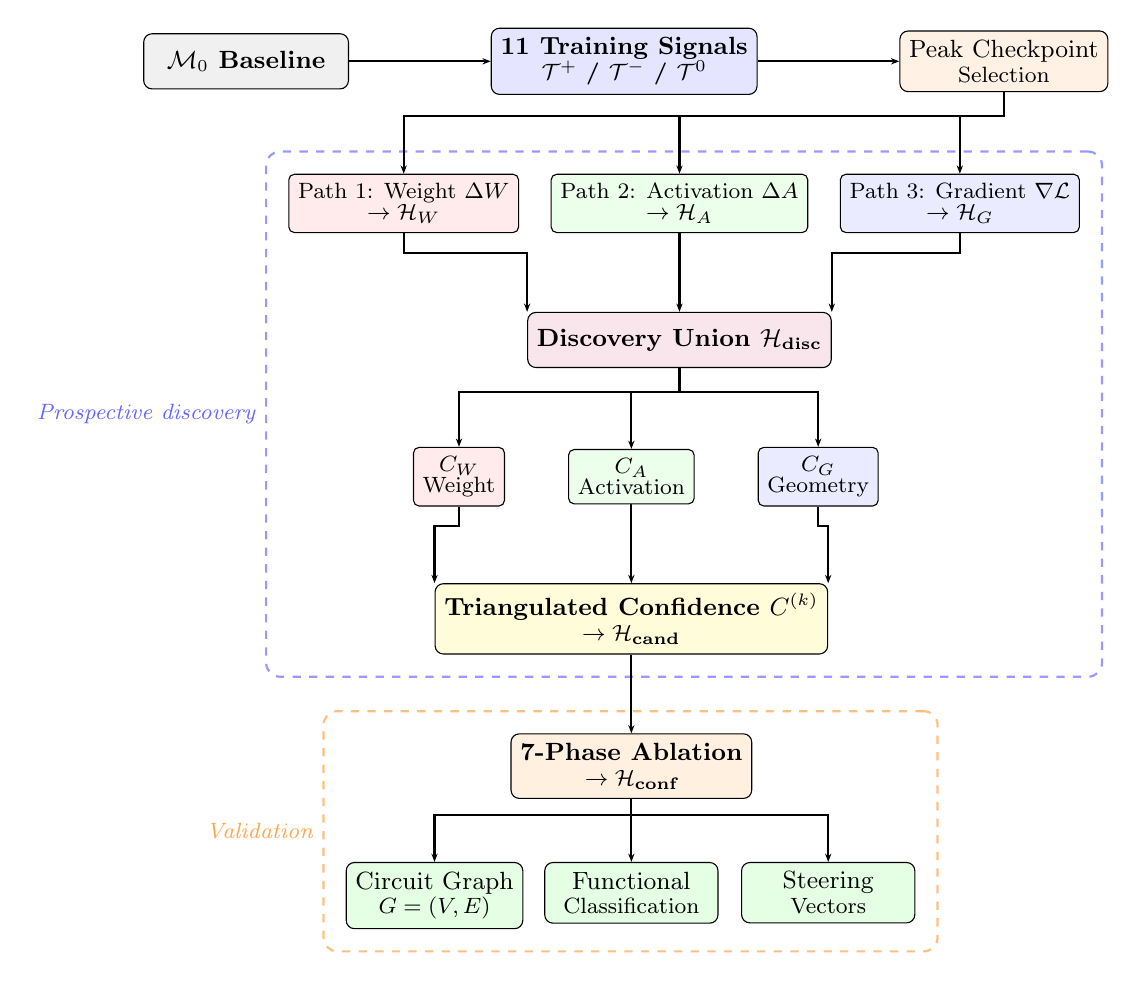
\begin{tikzpicture}[
    node distance=0.6cm and 0.8cm,
    >={Stealth[length=3pt]},
    box/.style={draw, rounded corners=3pt, minimum height=0.7cm, minimum width=2.2cm, font=\small, align=center, fill=#1},
    box/.default=white,
    phase/.style={draw, rounded corners=3pt, minimum height=0.7cm, minimum width=2.6cm, font=\small\bfseries, align=center, fill=#1},
    phase/.default=blue!8,
    smallbox/.style={draw, rounded corners=2pt, minimum height=0.55cm, font=\footnotesize, align=center, fill=#1},
    smallbox/.default=white,
    arr/.style={->, thick},
    darr/.style={->, thick, dashed},
]

% Row 1: Baseline and Signals
\node[phase=gray!12] (baseline) {$\mathcal{M}_0$ Baseline};
\node[phase=blue!10, right=1.8cm of baseline] (signals) {11 Training Signals\\[-2pt]{\footnotesize $\mathcal{T}^+$ / $\mathcal{T}^-$ / $\mathcal{T}^0$}};
\node[box=orange!10, right=1.8cm of signals] (peak) {Peak Checkpoint\\[-2pt]{\footnotesize Selection}};

\draw[arr] (baseline) -- (signals);
\draw[arr] (signals) -- (peak);

% Row 2: Three discovery paths
\node[smallbox=red!8, below=1.0cm of signals, xshift=-2.8cm] (pathW) {Path 1: Weight $\Delta W$\\[-2pt]{\footnotesize $\to \mathcal{H}_W$}};
\node[smallbox=green!8, right=0.4cm of pathW] (pathA) {Path 2: Activation $\Delta A$\\[-2pt]{\footnotesize $\to \mathcal{H}_A$}};
\node[smallbox=blue!8, right=0.4cm of pathA] (pathG) {Path 3: Gradient $\nabla\mathcal{L}$\\[-2pt]{\footnotesize $\to \mathcal{H}_G$}};

\draw[arr] (peak.south) -- ++(0,-0.3) -| (pathW.north);
\draw[arr] (peak.south) -- ++(0,-0.3) -| (pathA.north);
\draw[arr] (peak.south) -- ++(0,-0.3) -| (pathG.north);

% Row 3: Union and Domain Confidence
\node[phase=purple!10, below=1.0cm of pathA] (union) {Discovery Union $\mathcal{H}_{\text{disc}}$};

\draw[arr] (pathW.south) -- ++(0,-0.25) -| (union.north west);
\draw[arr] (pathA.south) -- (union.north);
\draw[arr] (pathG.south) -- ++(0,-0.25) -| (union.north east);

% Row 4: Three domain confidences
\node[smallbox=red!8, below=1.0cm of union, xshift=-2.8cm] (CW) {$C_W$\\[-2pt]{\footnotesize Weight}};
\node[smallbox=green!8, right=0.8cm of CW] (CA) {$C_A$\\[-2pt]{\footnotesize Activation}};
\node[smallbox=blue!8, right=0.8cm of CA] (CG) {$C_G$\\[-2pt]{\footnotesize Geometry}};

\draw[arr] (union.south) -- ++(0,-0.3) -| (CW.north);
\draw[arr] (union.south) -- ++(0,-0.3) -| (CA.north);
\draw[arr] (union.south) -- ++(0,-0.3) -| (CG.north);

% Row 5: Triangulation
\node[phase=yellow!15, below=1.0cm of CA] (tri) {Triangulated Confidence $C^{(k)}$\\[-2pt]{\footnotesize $\to \mathcal{H}_{\text{cand}}$}};

\draw[arr] (CW.south) -- ++(0,-0.25) -| (tri.north west);
\draw[arr] (CA.south) -- (tri.north);
\draw[arr] (CG.south) -- ++(0,-0.25) -| (tri.north east);

% Row 6: Ablation and outputs
\node[phase=orange!12, below=1.0cm of tri] (ablation) {7-Phase Ablation\\[-2pt]{\footnotesize $\to \mathcal{H}_{\text{conf}}$}};
\draw[arr] (tri) -- (ablation);

% Final outputs
\node[box=green!10, below=0.8cm of ablation, xshift=-2.5cm] (graph) {Circuit Graph\\[-2pt]{\footnotesize $G = (V, E)$}};
\node[box=green!10, below=0.8cm of ablation] (class) {Functional\\[-2pt]{\footnotesize Classification}};
\node[box=green!10, below=0.8cm of ablation, xshift=2.5cm] (steer) {Steering\\[-2pt]{\footnotesize Vectors}};

\draw[arr] (ablation.south) -- ++(0,-0.2) -| (graph.north);
\draw[arr] (ablation.south) -- (class.north);
\draw[arr] (ablation.south) -- ++(0,-0.2) -| (steer.north);

% Side annotation: prospective vs post-hoc boundary
\begin{scope}[on background layer]
\node[draw=blue!40, dashed, thick, rounded corners=5pt, inner sep=8pt,
      fit=(pathW)(pathA)(pathG)(union)(CW)(CA)(CG)(tri),
      label={[font=\footnotesize\itshape, text=blue!60, align=center]left:Prospective discovery}] {};
\node[draw=orange!50, dashed, thick, rounded corners=5pt, inner sep=8pt,
      fit=(ablation)(graph)(class)(steer),
      label={[font=\footnotesize\itshape, text=orange!70, align=center]left:Validation}] {};
\end{scope}

\end{tikzpicture}
\caption{The DCAF pipeline. Training signals produce weight deltas, activation changes, and gradients that feed three independent discovery paths. Discovered components receive confidence scores from all three measurement domains, triangulated into a unified score. Candidates are then validated through a 7-phase ablation protocol, producing a circuit graph with functional classifications and steering vectors. The dashed boundaries highlight DCAF's key architectural distinction: circuit candidates are identified \emph{prospectively} through training perturbations, with ablation serving as \emph{validation} rather than discovery.}
\label{fig:pipeline}
\end{figure}

%%%%%%%%%%%%%%%%%%%%%%%%%%%%%%%%%%%%%%%%%%%%%%%%%%%%%%%%%%%%%%%%%%%%%%%%%%%%%%%
\section{Multi-Path Discovery}
\label{sec:multi-path-discovery}
%%%%%%%%%%%%%%%%%%%%%%%%%%%%%%%%%%%%%%%%%%%%%%%%%%%%%%%%%%%%%%%%%%%%%%%%%%%%%%%

DCAF uses percentile-based significance predicates to determine whether a projection's weight delta is large enough to be considered behaviorally relevant. A projection is \emph{significant} if its RMS-normalized delta norm exceeds the $\tau_{\text{sig}} = 85$th percentile across all projections; it is \emph{insignificant} (for baseline filtering) if its norm falls below the $\tau_{\text{base}} = 50$th percentile. Full definitions of the percentile threshold function, all configurable parameters, and their rationale appear in Appendix~\ref{app:significance}.



DCAF employs three complementary discovery paths. Each path identifies candidate projections using different evidence, which are then mapped to components via $\mu_{\text{proj}}$. This section provides the discovery formulas with brief explanations; full methodology details are in the domain analysis sections (\S\ref{sec:weight-analysis}--\S\ref{sec:geometry-analysis}). All discovered components then receive confidence scores from all three measurement domains.

\subsection{Path 1: Weight-Based Discovery ($\mathcal{H}_W$)}
\label{sec:weight-discovery}

Weight-based discovery identifies projections that changed substantially during behavioral training---the most direct evidence of optimization pressure. Full methodology for computing these terms is in \S\ref{sec:weight-analysis}.

\begin{definition}[Signal Presence]
\label{def:signal-presence}
Counts how many training signals produced significant changes at a projection:
\begin{equation}
n^{(\text{proj})} = \sum_{i \in \mathcal{T}} \text{sig}(\text{proj}, i)
\end{equation}
where $\text{sig}(\text{proj}, i)$ tests if the RMS-normalized delta norm of the weight delta exceeds the significance threshold.
\end{definition}

\begin{definition}[Signal Effectiveness]
\label{def:signal-effectiveness-discovery}
Measures how successfully each training signal achieved behavioral change:
\begin{equation}
\text{eff}(i) = \text{normalize}_{[0,1]}\left(\Delta_{\text{improve}}(i) + \beta \cdot \text{threshold}(i)\right)
\end{equation}
where $\Delta_{\text{improve}}$ is the normalized improvement (loss reduction for SFT, margin improvement for preference methods) and $\text{threshold}(i)$ rewards training that crossed a behavioral threshold. See \S\ref{sec:weight-analysis} for full formulas.
\end{definition}

\begin{definition}[Aggregated Cluster Deltas]
\label{def:cluster-deltas}
For a projection, the effectiveness-weighted average delta matrix from each behavioral cluster:
\begin{equation}
\bar{\delta}^{(\text{proj})}_+ = \frac{\sum_{i \in \mathcal{T}^+} \text{eff}(i) \cdot \Delta W^{(\text{proj})}_i}{\sum_{i \in \mathcal{T}^+} \text{eff}(i)}, \quad \bar{\delta}^{(\text{proj})}_- = \frac{\sum_{j \in \mathcal{T}^-} \text{eff}(j) \cdot \Delta W^{(\text{proj})}_j}{\sum_{j \in \mathcal{T}^-} \text{eff}(j)}
\end{equation}
Each cluster delta is a full matrix of the same shape as the projection weight matrix, representing the net direction and magnitude of change induced by target vs.\ opposite behavioral training.
\end{definition}

\begin{definition}[Opposition Degree]
\label{def:opposition-degree}
Measures bidirectional control strength---how strongly a projection is pushed in opposite directions by the two behavioral clusters. Computed via cosine similarity on the flattened delta matrices:
\begin{equation}
\text{cos\_opp}^{(\text{proj})} = \cos\!\left(\text{flatten}(\bar{\delta}^{(\text{proj})}_+),\; \text{flatten}(\bar{\delta}^{(\text{proj})}_-)\right)
\end{equation}
\begin{equation}
\text{opp\_degree}(\text{proj}) = \max\!\left(0,\; -\text{cos\_opp}^{(\text{proj})}\right)
\end{equation}
When $\mathcal{T}^+$ and $\mathcal{T}^-$ push the projection in opposite directions, $\text{cos\_opp} \approx -1$ and $\text{opp\_degree} \approx 1$. When they push in the same direction, $\text{cos\_opp} \approx +1$ and $\text{opp\_degree} = 0$. If either cluster delta has near-zero norm ($< 10^{-8}$), both values are 0. Cosine similarity is self-normalizing, requiring no layer-specific calibration.
\end{definition}

\begin{definition}[Weight-Based Discovery Score]
\label{def:weight-based-discovery-score}
Combines signal presence with opposition as additive bonus, with baseline filtering:
\begin{equation}
S^{(\text{proj})}_W = \min\left(1,\, \frac{\sum_{i \in \mathcal{T} \setminus \mathcal{T}^0} \text{eff}(i)^q \cdot \text{sig}(\text{proj}, i)}{\sum_{i \in \mathcal{T} \setminus \mathcal{T}^0} \text{eff}(i)^q} + \alpha \cdot \text{opp\_degree}(\text{proj})\right) \cdot \mathbf{1}\left[\forall t \in \mathcal{T}^0: \overline{\text{sig}}(\text{proj}, t)\right]
\end{equation}
where $q=2$ (effectiveness power), $\alpha=0.2$ (opposition bonus weight). The baseline filter (indicator) excludes projections responding to any neutral training.
\end{definition}

\begin{definition}[Weight-Based Discovery Set]
\label{def:weight-based-discovery-set}
Projections discovered via weight changes, mapped to components:
\begin{equation}
\mathcal{H}_W = \{\text{proj} \in \mathcal{P} : S^{(\text{proj})}_W \geq \tau_W\}
\end{equation}
where $\tau_W$ is the weight discovery threshold (default: 0.3).
\end{definition}

\begin{definition}[Bidirectionality Status]
\label{def:bidirectionality-status}
Flags projections showing sufficient opposition:
\begin{equation}
\text{bidirectional}(\text{proj}) = \mathbf{1}\left[\text{opp\_degree}(\text{proj}) > \tau_{\text{opp}}\right]
\end{equation}
where $\tau_{\text{opp}} = 0.3$ (default). A component is bidirectional if any of its projections exceeds $\tau_{\text{opp}}$.
\end{definition}

\subsection{Path 2: Activation-Based Discovery ($\mathcal{H}_A$)}
\label{sec:activation-discovery}

Activation-based discovery identifies \textbf{leverage points}: projections where small weight changes produce large representational effects. These are missed by weight-based discovery but may be critical for behavioral control. This path uses activation methodology from \S\ref{sec:activation-analysis}.

\begin{definition}[Component Activation Magnitude]
\label{def:component-activation-magnitude-discovery}
For component $k$, aggregate activation changes across signals and probe types:
\begin{equation}
m^{(k)}_{\text{agg}} = \frac{1}{|\mathcal{T}|} \sum_{i \in \mathcal{T}} \frac{1}{|\Pi|} \sum_{\pi \in \Pi} m^{(k,\pi)}_i
\end{equation}
where $m^{(k,\pi)}_i$ is the activation magnitude (see \S\ref{sec:activation-analysis}). Activations are hooked at component output level.
\end{definition}

\begin{definition}[Component Screening]
\label{def:component-screening}
Flag components with notable activation changes using a generous threshold:
\begin{equation}
\mathcal{K}_{\text{flagged}} = \left\{k \in \mathcal{K} : m^{(k)}_{\text{agg}} \geq \Phi_{\tau_{\text{comp}}}\left(\{m^{(k')}_{\text{agg}}\}_{k' \in \mathcal{K}}\right)\right\}
\end{equation}
where $\tau_{\text{comp}} = 70$ (default). The 70th percentile is deliberately generous to avoid missing leverage points.
\end{definition}

\begin{definition}[Projection-Level Activation Score]
\label{def:projection-level-activation-score}
For projections within flagged components, compute a score reflecting both the component's activation impact and the projection's weight magnitude (projections with larger norms have more leverage over activations):
\begin{equation}
S^{(\text{proj})}_A = \begin{cases}
\displaystyle\frac{m^{(\mu_{\text{proj}}(\text{proj}))}_{\text{agg}}}{\max_{k \in \mathcal{K}} m^{(k)}_{\text{agg}}} \cdot w_{\text{proj}}(\text{proj}) & \text{if } \mu_{\text{proj}}(\text{proj}) \in \mathcal{K}_{\text{flagged}} \\[1em]
0 & \text{otherwise}
\end{cases}
\end{equation}
where $w_{\text{proj}}(\text{proj}) = \|W^{(\text{proj})}\|_F \;/\; \max_{\text{proj}': \mu_{\text{proj}}(\text{proj}') = \mu_{\text{proj}}(\text{proj})} \|W^{(\text{proj}')}\|_F$ is the projection's relative weight norm within its component.
\end{definition}

\begin{definition}[Activation-Based Discovery Set]
\label{def:activation-based-discovery-set}
Projections discovered via activation analysis:
\begin{equation}
\mathcal{H}_A = \left\{\text{proj} \in \mathcal{P} : \mu_{\text{proj}}(\text{proj}) \in \mathcal{K}_{\text{flagged}} \land S^{(\text{proj})}_A \geq \Phi_{\tau_{\text{act}}}\left(\{S^{(\text{proj}')}_A\}_{\text{proj}': \mu_{\text{proj}}(\text{proj}') \in \mathcal{K}_{\text{flagged}}}\right)\right\}
\end{equation}
The 85th percentile within flagged components captures the most impactful projections.
\end{definition}

\begin{remark}[Two-Stage Design]
\label{rem:two-stage-activation-discovery}
The two-stage design (generous component screening, strict projection filtering) balances coverage against cost. Without screening, every projection would require analysis; the 70th percentile flags $\sim$30\% of components. This catches leverage points (small $\|\Delta W\|_{\text{RMS}}$, large $\|\Delta A\|$) that Path 1 misses.
\end{remark}

\begin{remark}[Activation Discovery Granularity]
\label{rem:activation-discovery-granularity}
Path 2 operates at component level for discovery (activation hooks capture at head/MLP output) and uses weight norm as a heuristic proxy for projection-level attribution. This proxy assumes projections with larger weight norms have more leverage over component activations. While reasonable, this is not causal projection-level attribution. The projection-level evidence for activation-discovered components comes from the weight and geometry domains during confidence scoring, not from the activation path itself.
\end{remark}

\subsection{Path 3: Gradient-Based Discovery ($\mathcal{H}_G$)}
\label{sec:gradient-discovery}

Gradient-based discovery identifies projections with \textbf{high behavioral gradients}: projections that would affect behavior if modified, regardless of whether training actually changed them. This is purely mathematical prediction, complementing the empirical observation of Paths 1 and 2.

\begin{definition}[Behavioral Objective]
\label{def:behavioral-objective}
For each training signal $t_i$, let $\mathcal{O}_i$ denote the objective function that signal optimizes:
\begin{equation}
\mathcal{O}_i = \begin{cases}
\mathbb{E}_{x \sim D_i}[-\log p(y|x)] & \text{if } t_i \in \{\text{SFT signals}\} \\[0.5em]
-\mathbb{E}_{(x,y_w,y_l) \sim D_i}[M(y_w, y_l | x)] & \text{if } t_i \in \{\text{DPO, SimPO signals}\} \\[0.5em]
-\mathbb{E}_{x \sim D_i}[R(x)] & \text{if } t_i \in \{\text{RL signals}\} \\[0.5em]
-\mathbb{E}_{x \sim D_i}[\mathbb{E}_{y \sim \pi}[R(x,y)]] & \text{if } t_i \in \{\text{GRPO signals}\}
\end{cases}
\end{equation}
where $M$ is the preference margin, $R$ is the reward, and negation converts maximization objectives to minimization form. Signal-specific formulations match those in Definition~\ref{def:signal-effectiveness}.
\end{definition}

\begin{definition}[Behavioral Gradient]
\label{def:behavioral-gradient}
For a projection, compute the effectiveness-weighted behavioral gradient magnitude. The gradient of $\mathcal{O}_i$ with respect to the projection weight matrix is itself a matrix of the same shape; its RMS-normalized Frobenius norm measures the total sensitivity:
\begin{equation}
g^{(\text{proj})} = \sum_{i \in \mathcal{T}^+ \cup \mathcal{T}^-} \text{eff}(i) \cdot \left\|\frac{\partial \mathcal{O}_i}{\partial W^{(\text{proj})}}\right\|_{\text{RMS}}
\end{equation}
RMS normalization (Definition~\ref{def:rms-norm}) eliminates the same dimensional bias as in the weight domain: without it, larger projections would systematically produce larger gradient norms regardless of behavioral sensitivity. Gradients are computed at $\mathcal{M}_0$ on the behavioral training data, measuring how sensitive each projection is to the behavioral objective at the starting point.
\end{definition}

\begin{definition}[Gradient-Based Discovery Set]
\label{def:gradient-based-discovery-set}
Projections discovered via gradient analysis:
\begin{equation}
\mathcal{H}_G = \left\{\text{proj} \in \mathcal{P} : g^{(\text{proj})} \geq \Phi_{\tau_{\text{grad}}}\left(\{g^{(\text{proj}')}\}_{\text{proj}' \in \mathcal{P}}\right)\right\}
\end{equation}
where $\tau_{\text{grad}} = 85$ (default).
\end{definition}

\begin{remark}[Gradient Discovery Interpretation]
\label{rem:gradient-discovery-interpretation}
Path 3 discovers projections that the loss landscape identifies as behaviorally relevant, independent of training dynamics:
\begin{itemize}[nosep]
\item High gradient, low weight change: Projection is relevant but optimization didn't modify it (possibly due to regularization, learning rate, or saddle points)
\item High gradient, high weight change: Converging evidence from mathematical prediction and empirical observation
\item Low gradient, high weight change: Weight changed but not due to behavioral pressure (possible confound)
\end{itemize}
Gradient-based discovery is purely predictive---it identifies what \emph{could} affect behavior. Ablation confirms what \emph{does} affect behavior.
\end{remark}

\subsection{Discovery Integration}
\label{sec:discovery-integration}

\begin{definition}[Unified Discovery Set]
\label{def:unified-discovery-set}
Each discovery path returns a set of projection IDs. These are mapped to components via $\mu_{\text{proj}}$ and unioned:
\begin{equation}
\mathcal{H}_{\text{disc}} = \text{components}(\mathcal{H}_W) \cup \text{components}(\mathcal{H}_A) \cup \text{components}(\mathcal{H}_G)
\end{equation}
where $\text{components}(S) = \{\mu_{\text{proj}}(\text{proj}) : \text{proj} \in S\}$. Discovery is inclusive: a component flagged by \emph{any} path becomes a candidate for confidence scoring and ablation validation.
\end{definition}

\begin{definition}[Component Discovery Attribution]
\label{def:component-discovery-attribution}
For each component $k \in \mathcal{H}_{\text{disc}}$, record which discovery paths flagged it and aggregate projection-level scores:
\begin{align}
\text{disc\_paths}(k) &= \{W : \exists\, \text{proj} \in \mu_{\text{proj}}^{-1}(k) \cap \mathcal{H}_W\} \cup \{A : \exists\, \text{proj} \in \mu_{\text{proj}}^{-1}(k) \cap \mathcal{H}_A\} \cup \{G : \exists\, \text{proj} \in \mu_{\text{proj}}^{-1}(k) \cap \mathcal{H}_G\} \\[0.5em]
\text{paths}(k) &= |\text{disc\_paths}(k)|
\end{align}
Component-level discovery scores are aggregated from projections via max:
\begin{equation}
S_W(k) = \max_{\text{proj} \in \mu_{\text{proj}}^{-1}(k) \cap \mathcal{H}_W} S^{(\text{proj})}_W, \qquad S_G(k) = \max_{\text{proj} \in \mu_{\text{proj}}^{-1}(k) \cap \mathcal{H}_G} g^{(\text{proj})}
\end{equation}
The activation score $S_A(k) = m^{(k)}_{\text{agg}} / \max_{k'} m^{(k')}_{\text{agg}}$ is already component-level. Multi-path discovery ($\text{paths}(k) \geq 2$) indicates converging evidence from independent methods.
\end{definition}

\begin{remark}[Path Independence Principle]
\label{rem:path-independence-principle}
The three discovery paths are deliberately independent:
\begin{itemize}[nosep]
\item Path 1 uses weight deltas only
\item Path 2 uses activation deltas only (after component screening)
\item Path 3 uses gradients only
\end{itemize}
This independence means multi-path discovery is strong evidence: three different measurement approaches identified the same component as relevant. The unified confidence score (\S\ref{sec:unified-confidence}) incorporates a multi-path bonus to reflect this convergent evidence.
\end{remark}

\begin{remark}[Discovery vs.\ Confidence]
\label{rem:discovery-vs-confidence}
Discovery and confidence serve different purposes:
\begin{itemize}[nosep]
\item \textbf{Discovery} (this section): Which components should we analyze? Uses thresholds to filter.
\item \textbf{Confidence} (\S\ref{sec:unified-confidence}): How confident are we in each discovered component? Uses continuous scores from all three domains.
\end{itemize}
A component discovered via Path 2 (activation) still receives confidence contributions from the weight domain ($C_W$, \S\ref{sec:weight-analysis}), activation domain ($C_A$, \S\ref{sec:activation-analysis}), and geometry domain ($C_G$, \S\ref{sec:geometry-analysis}). Discovery determines \emph{what} to analyze; domain analysis determines \emph{strength of evidence}.
\end{remark}

%%%%%%%%%%%%%%%%%%%%%%%%%%%%%%%%%%%%%%%%%%%%%%%%%%%%%%%%%%%%%%%%%%%%%%%%%%%%%%%
\section{Weight Analysis}
\label{sec:weight-analysis}
%%%%%%%%%%%%%%%%%%%%%%%%%%%%%%%%%%%%%%%%%%%%%%%%%%%%%%%%%%%%%%%%%%%%%%%%%%%%%%%

This section provides full methodology for weight-based analysis. Discovery formulas appear in \S\ref{sec:weight-discovery}; this section covers implementation details, edge cases, and design rationale. All discovered components ($\mathcal{H}_{\text{disc}}$) receive weight confidence scores $C_W$, regardless of which path discovered them. Weight analysis operates at \textbf{projection level}: each projection matrix is analyzed individually, then results are aggregated to component level for integration with the other domains.

\subsection{Signal Effectiveness}

\begin{definition}[Signal Effectiveness---Full Formula]
\label{def:signal-effectiveness}
For training signal $t_i \in \mathcal{T}^+ \cup \mathcal{T}^-$, define the raw effectiveness score:
\begin{equation}
\text{eff}_{\text{raw}}(i) = \Delta_{\text{improve}}(i) + \beta \cdot \text{threshold}(i)
\end{equation}
where $\Delta_{\text{improve}}(i)$ is the normalized improvement metric, computed from the baseline model $\mathcal{M}_0$ to the peak checkpoint:
\begin{equation}
\Delta_{\text{improve}}(i) = \begin{cases}
\displaystyle\frac{\mathcal{L}_{\text{pre}}(i) - \mathcal{L}_{\text{peak}}(i)}{\mathcal{L}_{\text{pre}}(i)} & \text{if } t_i \in \{\text{SFT signals}\} \\[1em]
\displaystyle\frac{M_{\text{peak}}(i) - M_{\text{pre}}(i)}{|M_{\text{pre}}(i)| + \varepsilon} & \text{if } t_i \in \{\text{pairwise preference signals (DPO, SimPO, etc.)}\} \\[1em]
\displaystyle\frac{\mathbb{E}[R_{\text{peak}}(i)] - \mathbb{E}[R_{\text{pre}}(i)]}{|\mathbb{E}[R_{\text{pre}}(i)]| + \varepsilon} & \text{if } t_i \in \{\text{GRPO signals}\} \\[1em]
\displaystyle\frac{R_{\text{peak}}(i) - R_{\text{pre}}(i)}{|R_{\text{pre}}(i)| + \varepsilon} & \text{if } t_i \in \{\text{RL signals}\}
\end{cases}
\end{equation}
where $\mathcal{L}$ is task loss (SFT), $M$ is preference margin (DPO/SimPO), $\mathbb{E}[R]$ is expected reward over generated responses (GRPO), and $R$ is cumulative episode reward (RL). All ``peak'' subscripts refer to evaluation at the peak checkpoint $W_{i,\text{peak}}$ (\S\ref{sec:peak-checkpoint}).

The threshold bonus rewards training that achieves actual behavioral change:
\begin{equation}
\text{threshold}(i) = \begin{cases}
1 & \text{if peak checkpoint crosses behavioral threshold} \\
0 & \text{otherwise}
\end{cases}
\end{equation}
Examples: preference margin $M_{\text{peak}} > 0$, refusal rate exceeds target percentage, reward exceeds baseline. The threshold bonus weight $\beta$ (default: $\beta = 0.4$) distinguishes ``trained hard but didn't implement behavior'' from ``actually achieved behavioral change.''

Normalize to $[0,1]$ with outlier handling via clipping at 95th percentile:
\begin{equation}
\text{eff}(i) = \max\left(0, \frac{\text{eff}_{\text{raw}}(i) - \min_j \text{eff}_{\text{raw}}(j)}{\text{clip}_{95}(\max_j \text{eff}_{\text{raw}}(j)) - \min_j \text{eff}_{\text{raw}}(j)}\right)
\end{equation}
Negative effectiveness (training degradation) is clipped to zero.
\end{definition}

\begin{remark}[Effectiveness Power Parameter]
\label{rem:effectiveness-power-parameter}
Effectiveness is defined once with the threshold bonus, then different powers are applied based on context:
\begin{itemize}[nosep]
\item \textbf{Aggregated cluster deltas:} Use $\text{eff}(i)^1$ (linear). When computing average deltas, all effective signals contribute proportionally---we want accurate direction estimates.
\item \textbf{Weight confidence:} Use $\text{eff}(i)^q$ with $q=2$ (power transform). When determining confidence, successful runs should dominate over failed runs.
\end{itemize}
The threshold bonus (via $\beta$) applies everywhere through the base effectiveness; the power parameter $q$ controls emphasis in confidence weighting.
\end{remark}

\subsection{RMS Normalization of Projection Deltas}
\label{sec:rms-normalization}

\begin{definition}[RMS-Normalized Frobenius Norm]
\label{def:rms-norm}
For a projection weight delta matrix $\Delta W_i^{(\text{proj})} \in \mathbb{R}^{m \times n}$, the RMS-normalized Frobenius norm is:
\begin{equation}
\|\Delta W_i^{(\text{proj})}\|_{\text{RMS}} = \frac{\|\Delta W_i^{(\text{proj})}\|_F}{\sqrt{m \cdot n}}
\end{equation}
where $(m, n)$ is the projection matrix shape. This equals the root-mean-square of all elements in the delta matrix: $\sqrt{\frac{1}{mn}\sum_{a,b}(\Delta W_{a,b})^2}$. All weight-domain significance comparisons ($\text{sig}$, $\overline{\text{sig}}$, $S_W$, $C_W$) use $\|\cdot\|_{\text{RMS}}$ in place of $\|\cdot\|_F$.
\end{definition}

\begin{remark}[Dimensional Bias Correction]
\label{rem:dimensional-bias-correction}
Raw Frobenius norms are systematically biased by projection dimensions. For Gemma 2 2B, an MLP gate projection ($2304 \times 9216$, $mn \approx 21.2$M parameters) produces $\sim$6$\times$ larger raw Frobenius norms than an attention Q projection ($2304 \times 256$, $mn \approx 0.59$M parameters) for identical per-element changes, because $\sqrt{21.2\text{M} / 0.59\text{M}} \approx 6.0$. Percentile-based significance thresholds applied to raw norms therefore systematically favor MLP projections and miss genuinely significant attention projection changes. Dividing by $\sqrt{m \cdot n}$ normalizes to per-element scale, eliminating this architectural bias. The normalizer is a deterministic architectural constant---always nonzero, precomputable once per model.
\end{remark}

\begin{definition}[Base-Relative Delta (Diagnostic Only)]
\label{def:base-relative-delta}
For diagnostic interpretation, compute the base-weight relative normalization:
\begin{equation}
\|\Delta W\|_{\text{rel}} = \frac{\|\Delta W\|_F}{\|W_0\|_F + \varepsilon_{\text{rms}}}
\end{equation}
where $W_0$ is the weight matrix of the configured baseline model $\mathcal{M}_0$ (Definition~\ref{def:baseline-model}) and $\varepsilon_{\text{rms}}$ (default: $10^{-8}$) prevents division by zero. This captures ``what fraction of the projection shifted.'' Stored as \texttt{base\_relative\_delta} in projection results. This metric is \textbf{not} used in any discovery or confidence formula---it is metadata for interpretation only.
\end{definition}

\begin{remark}[RMS vs.\ Relative Divergence]
\label{rem:rms-vs-relative-divergence}
When RMS and relative rankings diverge for a projection, the divergence is diagnostically informative:
\begin{center}
\begin{tabular}{lll}
\toprule
\textbf{Pattern} & \textbf{Condition} & \textbf{Interpretation} \\
\midrule
High RMS, low relative & Large $\|\Delta W\|_{\text{RMS}}$, small $\|\Delta W\|_{\text{rel}}$ & Large absolute change in \\
& & a high-magnitude projection \\
Low RMS, high relative & Small $\|\Delta W\|_{\text{RMS}}$, large $\|\Delta W\|_{\text{rel}}$ & Small-magnitude projection \\
& & shifted proportionally a lot \\
Both high & Large $\|\Delta W\|_{\text{RMS}}$ and $\|\Delta W\|_{\text{rel}}$ & Unambiguously significant \\
Both low & Small $\|\Delta W\|_{\text{RMS}}$ and $\|\Delta W\|_{\text{rel}}$ & Unambiguously insignificant \\
\bottomrule
\end{tabular}
\end{center}
\noindent Low-RMS / high-relative projections may warrant investigation despite failing significance thresholds---they represent proportionally large shifts in small-magnitude projections that RMS normalization, by design, does not upweight.
\end{remark}

\subsection{Opposition Degree}
\label{sec:opposition-degree}

\begin{definition}[Opposition Degree---Full Methodology]
\label{def:opposition-degree-full-methodology}
Opposition degree measures how strongly a projection is pushed in opposite directions by the two behavioral clusters. The measure uses cosine similarity on the flattened cluster delta matrices (Definition~\ref{def:cluster-deltas}):
\begin{equation}
\text{cos\_opp}^{(\text{proj})} = \cos\!\left(\text{flatten}(\bar{\delta}^{(\text{proj})}_+),\; \text{flatten}(\bar{\delta}^{(\text{proj})}_-)\right)
\end{equation}
\begin{equation}
\text{opp\_degree}(\text{proj}) = \max\!\left(0,\; -\text{cos\_opp}^{(\text{proj})}\right)
\end{equation}
The $\text{flatten}$ operation reshapes a matrix $\in \mathbb{R}^{m \times n}$ into a vector $\in \mathbb{R}^{mn}$, enabling cosine similarity to measure the directional relationship between the two cluster deltas in full weight space. If either cluster delta has near-zero Frobenius norm ($< 10^{-8}$), both $\text{cos\_opp}$ and $\text{opp\_degree}$ are set to 0.
\end{definition}

\begin{remark}[Why Cosine Similarity]
\label{rem:why-cosine-similarity}
Cosine similarity on flattened matrices is self-normalizing: it measures the \emph{direction} of change without being affected by magnitude differences between layers, projections, or training signals. This eliminates the need for layer-specific calibration.

High opposition ($\text{opp\_degree} \approx 1$) indicates the projection is a bidirectional control point---the same weight matrix mediates both the target behavior and its opposite, with $\mathcal{T}^+$ and $\mathcal{T}^-$ pushing in anti-aligned directions through the full weight space.
\end{remark}

\begin{remark}[SVD Diagnostics]
Optional SVD diagnostics on cluster delta matrices characterize the spectral structure of weight changes: rank-1 fraction measures how concentrated the change is along a single mapping, and spectral opposition measures whether $\mathcal{T}^+$ and $\mathcal{T}^-$ oppose along the dominant change direction. These do not enter the confidence formula. Full definitions appear in Appendix~\ref{app:svd-diagnostics}.
\end{remark}

\subsection{Weight Confidence}
\label{sec:weight-confidence}

\begin{definition}[Projection-Level Weight Confidence]
\label{def:projection-level-weight-confidence}
For any projection in a discovered component ($\mu_{\text{proj}}(\text{proj}) \in \mathcal{H}_{\text{disc}}$), the weight confidence uses the same formula as the discovery score:
\begin{equation}
C^{(\text{proj})}_W = \min\left(1,\, \frac{\sum_{i \in \mathcal{T} \setminus \mathcal{T}^0} \text{eff}(i)^q \cdot \text{sig}(\text{proj}, i)}{\sum_{i \in \mathcal{T} \setminus \mathcal{T}^0} \text{eff}(i)^q} + \alpha \cdot \text{opp\_degree}(\text{proj})\right) \cdot \mathbf{1}\left[\forall t \in \mathcal{T}^0: \overline{\text{sig}}(\text{proj}, t)\right]
\end{equation}

Computed for \emph{all} projections of discovered components, not just those in $\mathcal{H}_W$. The formula has three components:
\begin{itemize}[nosep]
\item \textbf{Signal presence} (first term): Effectiveness-weighted fraction of behavioral signals that changed this projection significantly. The power transform ($q=2$) makes successful training runs contribute much more than failed runs.
\item \textbf{Opposition bonus} ($\alpha \cdot \text{opp\_degree}$): Adds confidence when the projection shows bidirectional control.
\item \textbf{Baseline filter} (indicator): Zeros out confidence if the projection responds to neutral training, excluding general-purpose projections.
\end{itemize}
\end{definition}

\begin{definition}[Component-Level Weight Confidence]
\label{def:component-level-weight-confidence}
The component's weight confidence is the maximum across its projections:
\begin{equation}
C^{(k)}_W = \max_{\text{proj} \in \mu_{\text{proj}}^{-1}(k)} C^{(\text{proj})}_W
\end{equation}
The most implicated projection drives the component's weight confidence. If $W_V$ shows strong opposition, the head is behaviorally relevant regardless of what $W_Q$ does.
\end{definition}

\begin{remark}[Weight Confidence for Non-Weight Discoveries]
\label{rem:weight-confidence-for-non-weight-discoveries}
A component discovered via Path 2 (activation) with low $C_W$ indicates a leverage point: small weight changes produce large activation effects. A component discovered via Path 3 (gradient) with low $C_W$ indicates the gradient landscape predicted behavioral relevance but training didn't modify the component. Both patterns are scientifically interesting and worth investigating via ablation.
\end{remark}

%%%%%%%%%%%%%%%%%%%%%%%%%%%%%%%%%%%%%%%%%%%%%%%%%%%%%%%%%%%%%%%%%%%%%%%%%%%%%%%
\section{Activation Analysis}
\label{sec:activation-analysis}
%%%%%%%%%%%%%%%%%%%%%%%%%%%%%%%%%%%%%%%%%%%%%%%%%%%%%%%%%%%%%%%%%%%%%%%%%%%%%%%

This section provides full methodology for activation-based analysis. Discovery formulas appear in \S\ref{sec:activation-discovery}; this section covers probe types, activation capture, and confidence computation.

\subsection{Probe Types}
\label{sec:activation-probe-types}

\begin{definition}[Universal Probe Types]
\label{def:universal-probe-types}
The three probe types capture behavioral processing at different stages:
\begin{equation}
\Pi = \{\pi_{\text{detect}}, \pi_{\text{decide}}, \pi_{\text{eval}}\}
\end{equation}

\begin{samepage}
Abstract definitions:
\begin{description}[leftmargin=2em, nosep]
\item[$\pi_{\text{detect}}$:] \textbf{Behavioral trigger detection} (upstream) --- Does the model encode/recognize behavioral content?
\item[$\pi_{\text{decide}}$:] \textbf{Behavioral decision point} (middle) --- Does the model make the behavioral choice?
\item[$\pi_{\text{eval}}$:] \textbf{Behavioral path evaluation} (parallel) --- Does the model prefer the behavioral path?
\end{description}

Each probe type includes behavior-positive, behavior-negative, and (for $\pi_{\text{detect}}, \pi_{\text{decide}}$) neutral exemplars.
\end{samepage}
\end{definition}

\subsection{Activation Capture}
\label{sec:activation-capture}

\begin{definition}[Activation Snapshot]
\label{def:activation-snapshot}
An activation snapshot captures the internal representations at a specific component when the model processes probe inputs. Each row corresponds to one probe example, each column to one dimension of the component's activation space.
\begin{equation}
A^{(k,\pi)}_i \in \mathbb{R}^{n_\pi \times d_k}
\end{equation}
\end{definition}

\begin{definition}[Activation Delta and Magnitude]
\label{def:activation-delta-and-magnitude}
The activation delta measures how a component's representations changed after training relative to the baseline model $\mathcal{M}_0$ (Definition~\ref{def:baseline-model}). The magnitude $m$ summarizes this as a single scalar---the average norm of change across all probe examples---allowing comparison across components.
\begin{equation}
\Delta A^{(k,\pi)}_i = A^{(k,\pi)}_i - A^{(k,\pi)}_0, \qquad m^{(k,\pi)}_i = \frac{1}{n_\pi} \sum_{j=1}^{n_\pi} \left\|\Delta A^{(k,\pi)}_i[j]\right\|_2
\end{equation}
where $A^{(k,\pi)}_0$ denotes activations captured from $\mathcal{M}_0$.
\end{definition}

\begin{definition}[Component Significance]
\label{def:component-significance}
A component is significant for a given signal and probe if its activation magnitude exceeds the $\tau_{\text{act}}$ percentile across all components. This identifies components whose representations changed substantially relative to others.
\begin{equation}
\text{sig}_A(k, i, \pi) = \mathbf{1}\left[m^{(k,\pi)}_i \geq \Phi^A_{\tau_{\text{act}}}\left(\{m^{(k',\pi)}_i\}_{k' \in \mathcal{K}}\right)\right]
\end{equation}
\end{definition}

\subsection{Activation Confidence}
\label{sec:activation-confidence}

\begin{definition}[Activation Confidence $C_A$]
\label{def:activation-confidence}
Activation confidence measures what fraction of (signal, probe) combinations show significant activation changes at a component. Higher values indicate the component consistently responds to behavioral training across multiple signals and probe types.
\begin{equation}
n^{(k)}_A = \sum_{i \in \mathcal{T}} \sum_{\pi \in \Pi} \text{sig}_A(k, i, \pi), \qquad C^{(k)}_A = \frac{n^{(k)}_A}{|\mathcal{T}| \cdot |\Pi|}
\end{equation}
Activation confidence is inherently component-level throughout; hooks capture at head outputs and MLP outputs.
\end{definition}

\begin{remark}[Probe Construction: Matched Contrast Pairs]
\label{rem:probe-construction-matched-contrast-pairs}
Effective probe construction ideally uses \textbf{matched contrast pairs} where behavior-positive and behavior-negative inputs differ minimally, holding confounding features constant (topic, length, syntax, vocabulary, position). The gold standard is the ABC counterfactual design \citep{wang2023ioi}, where inputs differ by exactly 1--3 tokens. For example, in IOI circuit discovery, behavior-negative probes replace a single repeated name with a novel third name, removing the duplicate-token signal while preserving all other structure. When minimal-pair construction is not feasible for a given behavior, probes should be matched by distribution: balanced for length, topic, style, and format, so that the behavioral variable is the primary axis of variation. Poorly controlled probes---where positive and negative inputs differ in length, topic, or style---may cause DCAF to identify components that encode those confounds rather than the target behavior.
\end{remark}

\begin{remark}[No Opposition in Activation Domain]
\label{rem:no-opposition-in-activation-domain}
Activation criteria use significance only---no opposition predicate. High-dimensional activation vectors lack well-defined ``opposite direction.'' Opposition evidence comes from weight analysis (\S\ref{sec:weight-analysis}).
\end{remark}

%%%%%%%%%%%%%%%%%%%%%%%%%%%%%%%%%%%%%%%%%%%%%%%%%%%%%%%%%%%%%%%%%%%%%%%%%%%%%%%
\section{Geometry Analysis}
\label{sec:geometry-analysis}
%%%%%%%%%%%%%%%%%%%%%%%%%%%%%%%%%%%%%%%%%%%%%%%%%%%%%%%%%%%%%%%%%%%%%%%%%%%%%%%

The geometry domain analyzes how behavior is represented in activation space. It measures whether training created or strengthened directions that separate behavioral classes.

\subsection{Contrastive Direction Extraction}
\label{sec:contrastive-direction}

\begin{definition}[Activation Sets]
\label{def:activation-sets}
For component $k$ and model state $\mathcal{M}_i$:
\begin{align}
A^+_i(k) &= \{\text{activations on behavior-positive prompts}\} \\
A^-_i(k) &= \{\text{activations on behavior-negative prompts}\}
\end{align}
\end{definition}

\begin{definition}[Contrastive Direction Extraction Methods]
\label{def:contrastive-direction}
DCAF supports two canonical linear direction extractors.

\textbf{Difference-in-means (DiM).} The transparent baseline direction is the normalized class-mean difference:
\begin{equation}
d_{\text{DiM}} = \frac{\mu^+ - \mu^-}{\|\mu^+ - \mu^-\|}
\end{equation}

\textbf{Whitened SVD.} The default extractor uses the behavior-negative activations as the benign baseline covariance. Let $\mu^- = \mathbb{E}[A^-]$, $C_- = \text{Cov}(A^- - \mu^-)$, and eigendecompose $C_- = V\Lambda V^\top$. Retain dimensions
\begin{equation}
J = \{j : \lambda_j > \tau_{\text{eig}}\lambda_{\max}\}.
\end{equation}
Define the whitening projection:
\begin{equation}
P = V_J(\Lambda_J + \varepsilon_{\text{white}}I)^{-1/2}.
\end{equation}
For matched contrast pairs, compute the whitened difference matrix:
\begin{equation}
D_w = (A^+ - \mu^-)P - (A^- - \mu^-)P.
\end{equation}
Compute $D_w = U\Sigma R^\top$. The top-$r$ original-space directions are obtained by inverse-whitening the right singular vectors:
\begin{equation}
d_j = \frac{V_J(\Lambda_J + \varepsilon_{\text{white}}I)^{1/2} r_j}{\|V_J(\Lambda_J + \varepsilon_{\text{white}}I)^{1/2} r_j\|}.
\end{equation}
Default: \texttt{whitened\_svd}. Alternative: \texttt{dim}. Whitened SVD requires matched contrast pairs and a non-degenerate baseline covariance; failure to meet these requirements is reported rather than silently falling back to another extractor.
\end{definition}

\begin{definition}[Behavioral Subspace]
\label{def:behavioral-subspace}
For subspace dimension $r > 1$, let $U^{(k)}_i \in \mathbb{R}^{d_k \times r}$ be the top-$r$ discriminant directions from LDA or PCA on class-centered data.

Subspace similarity via principal angles $\theta_1, \ldots, \theta_r$:
\begin{equation}
\text{sim}(U_1, U_2) = \frac{1}{r} \sum_{j=1}^r \cos(\theta_j)
\end{equation}
\end{definition}

\begin{remark}[Subspace Extraction Methods]
\label{rem:subspace-extraction-methods}
Three approaches for extracting behavioral subspaces when $r > 1$:
\begin{description}[nosep, leftmargin=1em]
\item[Method 1 (PCA on class-centered data):] Center $A^+$ and $A^-$ by their respective means, concatenate, apply PCA. Top-$r$ components capture between-class variation.
\item[Method 2 (Multi-class LDA):] When more than two behavioral classes exist (e.g., target/opposite/neutral), multi-class LDA returns up to $(\text{num\_classes} - 1)$ discriminant directions.
\item[Method 3 (Linear probe weights):] Train a linear classifier on activations $\to$ behavior label. Apply SVD to the weight matrix; top-$r$ singular vectors define the subspace.
\end{description}
Default: Start with $r=1$. If cluster coherence is low, increase $r$.
\end{remark}

\subsection{LRS Components and Geometric Confidence}

The contrastive directions extracted above are evaluated through six metrics that together capture the quality, consistency, and validity of the behavioral representation at each component. These metrics are aggregated into the Linear Representation Score (LRS), which feeds into geometric confidence.

\begin{table}[h]
\centering
\small
\begin{tabular}{p{0.20\textwidth}p{0.40\textwidth}p{0.28\textwidth}}
\toprule
\textbf{LRS Component} & \textbf{What It Measures} & \textbf{Range and Ideal} \\
\midrule
Target coherence ($\text{coh}_+$) & Do $\mathcal{T}^+$ signals find the same direction? & $[0,1]$; high = consistent \\
Opposite coherence ($\text{coh}_-$) & Do $\mathcal{T}^-$ signals find the same direction? & $[0,1]$; high = consistent \\
Cross-cluster opposition ($\text{opp}$) & Do $\mathcal{T}^+$ and $\mathcal{T}^-$ directions oppose? & $[0,1]$; high = clean opposition \\
Baseline orthogonality ($\text{orth}$) & Is the direction independent of neutral training? & $[0,1]$; high = behavior-specific \\
Confound independence ($\rho_c$) & Is the direction free of known confounds? & $[0,1]$; high = uncontaminated \\
Predictivity gain ($\Delta_{\text{pred}}$) & Did training improve behavioral separability? & Rescaled to $[0,1]$ \\
\bottomrule
\end{tabular}
\caption{The six components of the Linear Representation Score. Each captures a different aspect of representational quality. All are clamped to $[0,1]$ before aggregation. Full formal definitions appear in Appendix~\ref{app:geometry-detail}.}
\label{tab:lrs-components}
\end{table}

\subsection{Linear Representation Score}

\begin{definition}[Linear Representation Score (LRS)]
\label{def:lrs}
The Linear Representation Score is a Hölder (power) mean of the six geometric metrics, providing a single number capturing the overall quality of linear behavioral representation at a component.

Let $x^{(k)}_1 = \text{coh}^{(k)}_+$, $x^{(k)}_2 = \text{coh}^{(k)}_-$, $x^{(k)}_3 = \text{opp}^{(k)}$, $x^{(k)}_4 = \text{orth}^{(k)}$, $x^{(k)}_5 = \rho^{(k)}_c$ (confound independence), $x^{(k)}_6 = \frac{1}{2}(\Delta_{\text{pred}}^{(k)} + 1)$ (scaled predictivity gain). Then:
\begin{equation}
\text{LRS}^{(k)} = \left(\frac{\sum_{i=1}^6 w_i \cdot (x^{(k)}_i + \varepsilon)^p}{\sum_{i=1}^6 w_i}\right)^{1/p}
\end{equation}

\begin{samepage}
Default parameters:
\begin{itemize}[nosep]
\item $p = 0.5$: Square-root mean (penalizes single bad component without being as harsh as geometric mean)
\item $\varepsilon = 0.05$: Smoothing to prevent zeros from dominating
\item $w_i = 1$ for all $i$: Equal weighting (sum to 6)
\end{itemize}
\end{samepage}

\noindent The power mean provides a tunable balance: low $p$ penalizes imbalance (requiring convergent evidence), while high $p$ is more forgiving of individual weak components. All components are clamped to $[0, 1]$ before aggregation: cosine-based terms via $\max(0, \cdot)$, predictivity gain via the $(1 + \Delta_{\text{pred}})/2$ rescaling. This ensures the power mean with fractional $p$ is well-defined. High LRS indicates clean linear representation of behavior.
\end{definition}

\begin{remark}[LRS Interpretation Thresholds]
\label{rem:lrs-interpretation-thresholds}
Interpretation guidelines:
\begin{itemize}[nosep]
\item $\text{LRS} > 0.7$: Strong linear representation of behavior
\item $\text{LRS} \in [0.4, 0.7]$: Moderate---some noise or non-linearity present
\item $\text{LRS} < 0.4$: Weak linear representation---behavior may be gated or distributed
\end{itemize}
\end{remark}

\subsection{Geometric Confidence}
\label{sec:geometric-confidence}

\begin{definition}[Geometric Confidence $C_G$]
\label{def:geometric-confidence}
Geometric confidence combines representational quality (LRS) with generalization ability. A component with high geometric confidence has a clean, consistent linear representation of the behavior that transfers to out-of-distribution examples.
\begin{equation}
C^{(k)}_G = \text{LRS}^{(k)} \cdot \text{gen}^{(k)}
\end{equation}
\end{definition}

\begin{remark}[Nonlinear Diagnostics]
\label{rem:nonlinear-diagnostics}
When $\text{LRS}^{(k)} < \tau_{\text{nonlinear}} = 0.4$, the behavioral representation may be nonlinear. DCAF triggers a suite of diagnostic methods---PaCMAP embedding with silhouette scoring, Procrustes alignment (structural mirror score), degree-2 polynomial probing, and kernel LDA---to characterize the nonlinearity without altering confidence scores or candidate status. Full definitions appear in Appendix~\ref{app:nonlinear}.
\end{remark}

%%%%%%%%%%%%%%%%%%%%%%%%%%%%%%%%%%%%%%%%%%%%%%%%%%%%%%%%%%%%%%%%%%%%%%%%%%%%%%%
% Direction Synthesis — extends Geometry Analysis to global residual stream
%%%%%%%%%%%%%%%%%%%%%%%%%%%%%%%%%%%%%%%%%%%%%%%%%%%%%%%%%%%%%%%%%%%%%%%%%%%%%%%

\subsection{Representation Direction Synthesis}
\label{sec:representation-direction-synthesis}

The preceding subsections extract per-component contrastive directions, measure their cross-signal consistency (LRS), and characterize nonlinear representations. This subsection extends that machinery to the \textbf{global residual stream}, producing validated behavioral directions backed by convergent evidence from all training signals. Existing methods (Arditi et al.\ 2024, Zou et al.\ 2024, Li et al.\ 2023, Marks \& Tegmark 2024) extract directions from a single contrast pair or training method with limited multi-signal validation. DCAF's multi-signal architecture eliminates this limitation.

The direction module synthesizes per-component contrastive directions (\S\ref{sec:contrastive-direction}), bidirectional steering vectors (\S\ref{sec:steering}), and activation deltas across all behavioral signals into global directions, layer trajectories, composition decompositions, and actionable intervention specifications. The entire pipeline is fully automated and behavior-agnostic.

\begin{remark}[Pipeline Placement]
\label{rem:direction-pipeline}
Direction extraction and DCS computation run at Step 6.5 in the pipeline (after per-component geometry analysis, before discovery). Composition analysis runs at Step 15.5 (after circuit graph reconstruction, requiring $\mathcal{H}_{\text{conf}}$). Both are described together here for conceptual coherence.
\end{remark}

\subsubsection{Global Direction Extraction}
\label{sec:direction-synthesis}
\label{sec:global-direction-extraction}

\begin{definition}[Residual Stream Hook Points]
\label{def:resid-hooks}
Register activation hooks at the residual stream after each layer's attention and MLP sub-layers:
\begin{equation}
R^{(L)}_{\text{post}} = \text{blocks}[L].\text{hook\_resid\_post} \in \mathbb{R}^{n \times d_{\text{model}}}
\end{equation}
for each layer $L \in \{0, \ldots, n_{\text{layers}} - 1\}$. These hooks are registered alongside the existing component-level hooks on the \emph{same forward passes}---zero additional forward pass cost.
\end{definition}

\begin{definition}[Multi-Position Capture and Selection]
\label{def:position-selection}
Rather than hardcoding a token position, capture residual stream activations at candidate positions $\mathcal{P} = \{-1, -2, -3, -5\}$ (relative to sequence end). Select automatically:
\begin{equation}
s^* = \arg\max_{s \in \mathcal{P}} \; \frac{1}{\binom{|\mathcal{T}^+|}{2}} \sum_{\substack{i,j \in \mathcal{T}^+ \\ i < j}} |\cos(d^{(L)}_i[s],\, d^{(L)}_j[s])|
\end{equation}
at the peak DCS layer $L^*$, where $d^{(L)}_i[s]$ is the contrastive direction extracted at position $s$ from signal $i$. The position with highest cross-signal agreement is selected.
\end{definition}

\begin{definition}[Per-Signal Direction Extraction]
\label{def:per-signal-direction}
For each training signal $t_i \in \mathcal{T}^+ \cup \mathcal{T}^-$ and each layer $L$, extract a contrastive direction from residual stream activations using whitened LDA (same method as Definition~\ref{def:contrastive-direction}, applied to residual stream instead of component outputs):
\begin{equation}
d^{(L)}_i = \frac{(\Sigma_w + \lambda I)^{-1}(\mu^+_i - \mu^-_i)}{\|(\Sigma_w + \lambda I)^{-1}(\mu^+_i - \mu^-_i)\|}
\end{equation}
where $\mu^+_i, \mu^-_i$ are the mean residual stream activations for target and opposite prompts under signal $t_i$, and $\Sigma_w$ is the pooled within-class covariance. This yields a direction matrix $D[\text{signal}][\text{layer}]$ containing up to $|\mathcal{T}^+ \cup \mathcal{T}^-| \times n_{\text{layers}}$ direction vectors.
\end{definition}

\subsubsection{Direction Convergence Score (DCS)}
\label{sec:dcs}

The Direction Convergence Score measures how strongly the training signals agree on a behavioral direction at each layer. It is structurally parallel to LRS (Definition~\ref{def:lrs}) but applied to global residual stream directions.

\begin{definition}[DCS Convergence Components]
\label{def:dcs-convergence}
For layer $L$, compute three convergence metrics:
\begin{align}
\text{coh}_+^{(L)} &= \frac{1}{\binom{|\mathcal{T}^+|}{2}} \sum_{\substack{i,j \in \mathcal{T}^+ \\ i < j}} |\cos(d^{(L)}_i, d^{(L)}_j)| & &\text{($\mathcal{T}^+$ within-cluster coherence)} \\[0.5em]
\text{coh}_-^{(L)} &= \frac{1}{\binom{|\mathcal{T}^-|}{2}} \sum_{\substack{i,j \in \mathcal{T}^- \\ i < j}} |\cos(d^{(L)}_i, d^{(L)}_j)| & &\text{($\mathcal{T}^-$ within-cluster coherence)} \\[0.5em]
\text{opp}^{(L)} &= \frac{1}{|\mathcal{T}^+||\mathcal{T}^-|} \sum_{\substack{i \in \mathcal{T}^+ \\ j \in \mathcal{T}^-}} \bigl(-\cos(d^{(L)}_i, d^{(L)}_j)\bigr) & &\text{(cross-cluster opposition)}
\end{align}
All three range $[0,1]$ for well-behaved directions ($[-1,1]$ in general). The convergence prerequisite is met when all three components $\geq \tau_{\text{dcs-conv}}$ (default: 0.3).
\end{definition}

\begin{definition}[Consensus Direction]
\label{def:consensus-direction}
When the convergence prerequisite is met, extract the consensus direction as the effectiveness-weighted mean of $\mathcal{T}^+$ directions:
\begin{equation}
d^{(L)}_{\text{consensus}} = \frac{\sum_{i \in \mathcal{T}^+} \text{eff}(i) \cdot d^{(L)}_i}{\|\sum_{i \in \mathcal{T}^+} \text{eff}(i) \cdot d^{(L)}_i\|}
\end{equation}
If the convergence prerequisite fails, no consensus direction is extracted.
\end{definition}

\begin{definition}[DCS Validation Components]
\label{def:dcs-validation}
Computed only when the convergence prerequisite is met (otherwise set to 0):
\begin{align}
\text{ortho}^{(L)} &= 1 - |\cos(d^{(L)}_{\text{consensus}},\, d^{(L)}_{\text{baseline}})| & &\text{(independence from baseline)} \\[0.5em]
\text{confound}^{(L)} &= 1 - \frac{1}{|\mathcal{D}_{\text{conf}}|}\sum_{d_c \in \mathcal{D}_{\text{conf}}} |\cos(d^{(L)}_{\text{consensus}},\, d_c)| & &\text{(independence from confounds)} \\[0.5em]
\text{pred}^{(L)} &= \text{AUC}_{\text{post}}^{(L)} - \text{AUC}_{\text{pre}}^{(L)} & &\text{(held-out prediction gain)}
\end{align}
where $d^{(L)}_{\text{baseline}}$ is the contrastive direction from the neutral signal ($t_{\text{DomainNative}}$; defaults to $\mathbf{0}$ yielding $\text{ortho} = 1$ if absent), $\mathcal{D}_{\text{conf}}$ is an optional set of confound directions (defaults to $\emptyset$ yielding $\text{confound} = 1$), and $\text{AUC}_{\text{pre/post}}$ are the classification AUCs on held-out behavioral prompts using projection onto $d_{\text{consensus}}$, measured from the baseline model $\mathcal{M}_0$ and after training respectively.
\end{definition}

\begin{definition}[DCS Aggregation]
\label{def:dcs-aggregation}
Aggregate the six components using the same power mean as LRS:
\begin{equation}
\text{DCS}(L) = \left[\frac{1}{6}\sum_{x \in \{\text{coh}_+, \text{coh}_-, \text{opp}, \text{ortho}, \text{confound}, \text{pred}\}} (x^{(L)} + \varepsilon)^p\right]^{1/p}
\end{equation}
with $p = 0.5$, $\varepsilon = 0.05$, uniform weights. All six components are clamped to $[0, 1]$ before aggregation, matching the LRS convention. If the convergence prerequisite fails, validation components are 0 and DCS bottoms out through the power mean.
\end{definition}

After consensus extraction, the DCS curve across layers reveals where the behavior crystallizes in the network. The peak DCS layer $L^* = \arg\max_L \text{DCS}(L)$ identifies where the behavioral direction is strongest. Composition analysis connects the circuit graph back to the global direction: each confirmed component's contribution is measured as $\text{contrib}(k) = \langle \Delta\text{output}^{(k)}, d^{(L^*)}_{\text{consensus}} \rangle$, where $\Delta\text{output}^{(k)}$ is the mean difference in component $k$'s output between target and opposite prompts. Full details of layer trajectory analysis, signal diagnostics, composition decomposition, intervention specification, and failure modes appear in Appendix~\ref{app:direction-synthesis-detail}.

%%%%%%%%%%%%%%%%%%%%%%%%%%%%%%%%%%%%%%%%%%%%%%%%%%%%%%%%%%%%%%%%%%%%%%%%%%%%%%%
\section{Training Diagnostics}
\label{sec:training-diagnostics}
%%%%%%%%%%%%%%%%%%%%%%%%%%%%%%%%%%%%%%%%%%%%%%%%%%%%%%%%%%%%%%%%%%%%%%%%%%%%%%%

Training diagnostics measure the quality of the training process itself, as opposed to the projection-level analysis in the preceding sections. Where weight, activation, and geometry analyses answer ``which projections implement the behavior?'' and ``how confident are we?'', training diagnostics answer ``did the training signals behave as expected?'' Poor training quality (e.g., inconsistent optimization trajectories, contradictory activation patterns) can undermine the reliability of downstream analysis even when individual metrics appear strong.

\subsection{Activation Delta Alignment}
\label{sec:activation-delta-alignment}

Activation delta alignment measures whether the training-induced activation changes are internally consistent. If multiple $T^+$ signals all aim to reinforce the same behavior, their activation deltas at behavioral components should point in similar directions. Likewise, $T^-$ deltas should be internally consistent and should oppose the $T^+$ direction.

\begin{definition}[Activation Delta Alignment]
\label{def:delta-alignment}
For component $k$, compute three alignment metrics from the activation deltas $\Delta A^{(k)}_i = A^{(k)}_{i,\text{peak}} - A^{(k)}_{i,\text{pre}}$:

\textbf{Within-cluster alignment (target):}
\begin{equation}
\text{align}^{(k)}_+ = \frac{1}{|\mathcal{T}^+|^2}\sum_{i,j \in \mathcal{T}^+} \cos(\Delta A^{(k)}_i, \Delta A^{(k)}_j)
\end{equation}

\textbf{Within-cluster alignment (opposite):}
\begin{equation}
\text{align}^{(k)}_- = \frac{1}{|\mathcal{T}^-|^2}\sum_{i,j \in \mathcal{T}^-} \cos(\Delta A^{(k)}_i, \Delta A^{(k)}_j)
\end{equation}

\textbf{Cross-cluster opposition:}
\begin{equation}
\text{oppose}^{(k)}_{\Delta} = \frac{1}{|\mathcal{T}^+||\mathcal{T}^-|}\sum_{i \in \mathcal{T}^+, j \in \mathcal{T}^-} \cos(\Delta A^{(k)}_i, \Delta A^{(k)}_j)
\end{equation}

Expected values for a well-behaved training process at behaviorally-relevant components:
\begin{itemize}[nosep]
\item $\text{align}_+ > 0.7$: Target signals move activations in the same direction.
\item $\text{align}_- > 0.7$: Opposite signals move activations in the same direction.
\item $\text{oppose}_\Delta < -0.5$: Target and opposite signals move activations in opposing directions.
\end{itemize}
\end{definition}

\begin{remark}[Activation Delta Alignment is Always Computed]
\label{rem:activation-delta-alignment-always-computed}
Unlike the optional curvature metrics below, activation delta alignment is always computed for every confirmed component. It provides a first-order sanity check on training consistency and is computationally inexpensive (cosine similarities between already-computed deltas). When $\text{align}_+$ or $\text{align}_-$ is low at a component that otherwise scores well, this flags possible inconsistency in the training signal suite worth investigating.
\end{remark}

\begin{remark}[Online Curvature Tracking (Optional)]
Online curvature tracking measures how winding the representational trajectory is during training relative to straight-line displacement. High curvature indicates competing gradients or unstable optimization; asymmetric curvature between $\mathcal{T}^+$ and $\mathcal{T}^-$ indicates one behavioral direction is easier to learn. This is an optional diagnostic requiring per-step monitoring. Full definitions appear in Appendix~\ref{app:curvature}.
\end{remark}

%%%%%%%%%%%%%%%%%%%%%%%%%%%%%%%%%%%%%%%%%%%%%%%%%%%%%%%%%%%%%%%%%%%%%%%%%%%%%%%
\section{Unified Confidence and Candidate Selection}
\label{sec:unified-confidence}
%%%%%%%%%%%%%%%%%%%%%%%%%%%%%%%%%%%%%%%%%%%%%%%%%%%%%%%%%%%%%%%%%%%%%%%%%%%%%%%

This section integrates evidence from all three discovery paths and all three measurement domains into unified confidence scores. All confidence scores are \textbf{component-level}.

\subsection{Base Triangulated Confidence}
\label{sec:base-triangulated-confidence}

\begin{definition}[Base Triangulated Confidence]
\label{def:base-triangulated-confidence}
For component $k \in \mathcal{H}_{\text{disc}}$, define the base triangulated confidence as a weighted geometric mean:
\begin{equation}
C^{(k)}_{\text{base}} = \left[(C^{(k)}_W + \varepsilon)^w \cdot (C^{(k)}_A + \varepsilon) \cdot (C^{(k)}_G + \varepsilon)\right]^{\frac{1}{w+2}}
\end{equation}
where $w \geq 1$ is the domain weight (default: $w = 2$) and $\varepsilon > 0$ is the smoothing parameter (default: $\varepsilon = 0.05$). $C^{(k)}_W$ is component-level (aggregated from projections via max), while $C^{(k)}_A$ and $C^{(k)}_G$ are already component-level.

The three measurement domains serve complementary roles:
\begin{itemize}[nosep]
\item $C_W$: Weight evidence---how much did projection weights change during behavioral training?
\item $C_A$: Activation evidence---how much did component representations change?
\item $C_G$: Geometric evidence---is there a clean behavioral direction at this component?
\end{itemize}
The weighted geometric mean with epsilon smoothing ensures: (1) all domains contribute but zeros don't completely dominate ($\varepsilon > 0$), and (2) domain agreement amplifies confidence. Smoothing can push the base score slightly above 1.0 when all domain scores are high; the $\min(1, \cdot)$ in the final unified confidence (Definition~\ref{def:final-unified-confidence}) enforces the $[0, 1]$ bound.
\end{definition}

\subsection{Multi-Path Discovery Bonus}
\label{sec:multi-path-discovery-bonus}

\begin{definition}[Multi-Path Discovery Bonus]
\label{def:multi-path-discovery-bonus}
Components discovered by multiple independent paths receive a confidence bonus reflecting converging evidence:
\begin{equation}
\text{bonus}(k) = \beta_{\text{path}} \cdot \max(0, \text{paths}(k) - 1)
\end{equation}
where $\text{paths}(k) = |\text{disc\_paths}(k)|$ and $\beta_{\text{path}} = 0.15$ (default).

This is additive rather than multiplicative to avoid penalizing single-path discoveries:
\begin{itemize}[nosep]
\item Single-path discovery: bonus $= 0$ (no penalty, no bonus)
\item Two-path discovery: bonus $= 0.15$ (converging evidence)
\item Three-path discovery: bonus $= 0.30$ (strong convergence)
\end{itemize}
\end{definition}

\begin{definition}[Final Unified Confidence]
\label{def:final-unified-confidence}
The complete confidence score combines base triangulated confidence with multi-path bonus:
\begin{equation}
C^{(k)} = \min(1, C^{(k)}_{\text{base}} + \text{bonus}(k))
\end{equation}
\end{definition}

\begin{remark}[Why Additive Bonus]
\label{rem:why-additive-bonus}
An additive bonus (rather than multiplicative) ensures:
\begin{itemize}[nosep]
\item Components discovered by only one path still get full domain confidence
\item Multi-path discovery provides additional evidence, not a requirement
\item The bonus is bounded and doesn't dominate domain confidence
\end{itemize}
A component found only by Path 2 (activation) with strong $C_A$ and $C_G$ but weak $C_W$ may still be high-confidence---it's a leverage point, not a false positive.
\end{remark}

\subsection{Candidate Set Construction}
\label{sec:candidate-set-construction}

\begin{definition}[Candidate Set]
\label{def:candidate-set}
Components with sufficient unified confidence:
\begin{equation}
\mathcal{H}_{\text{cand}} = \{k \in \mathcal{H}_{\text{disc}} : C^{(k)} \geq \tau_{\text{unified}}\}
\end{equation}
where $\tau_{\text{unified}}$ is the candidate threshold (default: 0.3).
\end{definition}

\begin{definition}[Confirmed Set]
\label{def:confirmed-set}
After ablation testing:
\begin{equation}
\mathcal{H}_{\text{conf}} = \{k \in \mathcal{H}_{\text{cand}} : \text{ablation affects behavior without breaking model}\}
\end{equation}
\end{definition}

\subsection{Domain Disagreement Analysis}
\label{sec:domain-disagreement-analysis}

\begin{remark}[Disagreement Diagnostics]
\label{rem:disagreement-diagnostics}
When domains disagree, the pattern reveals the component's nature:
\begin{itemize}[nosep]
\item \textbf{Weight high, Activation low:} Weights changed without representational reorganization (possibly dead or redundant projections)
\item \textbf{Weight low, Activation high:} Leverage point---small weight changes produce large representational effects
\item \textbf{Geometry high, Others low:} Pre-existing direction that training leveraged without creating new structure
\item \textbf{Gradient high, Weight low:} Gradient landscape predicted relevance but optimizer didn't modify (learning rate, regularization effects)
\end{itemize}
\end{remark}

\begin{remark}[Path-Domain Interaction Patterns]
\label{rem:path-domain-interaction-patterns}
The discovery path combined with domain confidence reveals component characteristics:

\begin{center}
\begin{tabular}{llll}
\toprule
\textbf{Discovered By} & $C_W$ & $C_A$ & \textbf{Interpretation} \\
\midrule
Path 1 only & High & High & Standard behavioral component \\
Path 1 only & High & Low & Weight change without activation effect \\
Path 2 only & Low & High & Leverage point \\
Path 3 only & Low & Low & Gradient prediction, needs ablation validation \\
Paths 1+2 & High & High & Strong converging evidence \\
Paths 2+3 & Low & High & Leverage point confirmed by gradients \\
All paths & High & High & Highest confidence \\
\bottomrule
\end{tabular}
\end{center}
\end{remark}

%%%%%%%%%%%%%%%%%%%%%%%%%%%%%%%%%%%%%%%%%%%%%%%%%%%%%%%%%%%%%%%%%%%%%%%%%%%%%%%
\section{Circuit Graph Reconstruction}
\label{sec:circuit-graph}
%%%%%%%%%%%%%%%%%%%%%%%%%%%%%%%%%%%%%%%%%%%%%%%%%%%%%%%%%%%%%%%%%%%%%%%%%%%%%%%

\begin{definition}[Circuit Nodes]
\label{def:circuit-nodes}
Confirmed behaviorally-relevant components:
\begin{equation}
V = \mathcal{H}_{\text{conf}}
\end{equation}
\end{definition}

\subsection{Edge Discovery Methods}
\label{sec:edge-discovery-methods}

\begin{definition}[Method 1: Activation Flow Analysis]
\label{def:edge-activation-flow-analysis}
Track activation correlation across layers:
\begin{equation}
\text{corr}^{(i)}(k, k') = \text{Corr}(A^{(k)}_i, A^{(k')}_i)
\end{equation}
Differential: Does correlation increase after training?
\end{definition}

\begin{definition}[Method 2: Targeted Ablation]
\label{def:edge-targeted-ablation}
Ablate component $k$, measure activation changes at other components:
\begin{equation}
E^{\text{abl}}_{k \to k'} = \|A^{(k')}_{\text{with } k} - A^{(k')}_{\text{without } k}\|_F
\end{equation}
\end{definition}

\begin{definition}[Method 3: Targeted Steering]
\label{def:edge-targeted-steering}
Apply steering vector at component $k$, measure activation changes:
\begin{equation}
E^{\text{steer}}_{k \to k'} = \|A^{(k')}_{\text{with } v_k} - A^{(k')}_{\text{without } v_k}\|_F
\end{equation}
\end{definition}

\begin{definition}[Method 4: Gradient Flow Analysis]
\label{def:edge-gradient-flow-analysis}
Track gradient correlation during training:
\begin{equation}
\text{grad\_corr}(k, k') = \text{Corr}(\nabla_{W_k} \mathcal{L}, \nabla_{W_{k'}} \mathcal{L})
\end{equation}
Shared gradient pressure suggests functional connection.
\end{definition}

\begin{definition}[Method 5: Cross-Layer Attention Patterns]
\label{def:edge-cross-layer-attention-patterns}
For attention heads, track information flow:
\begin{equation}
\text{attn\_flow}(k_\ell, k_{\ell'}) = \sum_s P_{\ell',h}[s, \text{pos}(k_\ell)]
\end{equation}
Measures whether downstream heads attend to positions where upstream components wrote.
\end{definition}

\begin{remark}[Screening vs.\ Causal Edge Evidence]
Methods 1, 4, and 5 (activation correlation, gradient correlation, attention flow) are \textbf{screening heuristics} that propose candidate edges for testing. They identify statistical associations, not causal relationships. Only Methods 2 and 3 (targeted ablation and targeted steering) produce \textbf{causal edge evidence}: they intervene on one component and measure the effect on another. The causal edge definition below uses only Methods 2 and 3.
\end{remark}

\begin{definition}[Causal Edge]
\label{def:causal-edge}
A causal edge exists between components when intervening on one (via ablation or steering) causally affects the other. The edge weight reflects the strength of this causal relationship, and the edge predicate applies a threshold to identify significant connections.
\begin{equation}
E_{k \to k'} = \max\left(E^{\text{abl}}_{k \to k'}, E^{\text{steer}}_{k \to k'}\right)
\end{equation}
\begin{equation}
e(k, k') = \mathbf{1}\left[E_{k \to k'} \geq \tau_E \land k' \in V\right]
\end{equation}
\end{definition}

\begin{definition}[Edge Pathway Attribution]
\label{def:edge-pathway-attribution}
For edges where the target component $k'$ is an attention head, determine which input pathway carries the causal signal:
\begin{enumerate}[nosep]
\item Ablate source component $k$
\item Hook $k'$'s Q, K, and V input projections separately
\item Measure $\|A^{(\text{proj})}_{\text{with}\;k} - A^{(\text{proj})}_{\text{without}\;k}\|_F$ at each hook
\item Normalize to pathway weights summing to 1.0:
\end{enumerate}
\begin{align}
w_Q &= \frac{\|\Delta A_Q\|_F}{\|\Delta A_Q\|_F + \|\Delta A_K\|_F + \|\Delta A_V\|_F} \\[0.3em]
w_K &= \frac{\|\Delta A_K\|_F}{\|\Delta A_Q\|_F + \|\Delta A_K\|_F + \|\Delta A_V\|_F} \\[0.3em]
w_V &= \frac{\|\Delta A_V\|_F}{\|\Delta A_Q\|_F + \|\Delta A_K\|_F + \|\Delta A_V\|_F}
\end{align}
For non-attention targets, the pathway is $\{$residual: 1.0$\}$. Edges in the circuit graph carry pathway metadata: $\text{via} = (w_Q, w_K, w_V)$.
\end{definition}

\begin{definition}[Behavioral Circuit Graph]
\label{def:behavioral-circuit-graph}
The behavioral circuit graph is the final output of DCAF's circuit reconstruction: a directed graph where nodes are confirmed behaviorally-relevant components and edges represent causal relationships discovered through intervention.
\begin{equation}
G = \left(V, \{(k, k') : e(k, k') = 1\}\right)
\end{equation}
\end{definition}

\begin{remark}[Circuit Graph Output Format]
\label{rem:circuit-graph-output-format}
The circuit graph is serialized as a JSON structure containing node metadata (discovery attribution, domain-level confidence scores, adaptive tiered functional classification, bidirectionality status) and edge metadata (causal weight, validation status, pathway attribution). An illustrative example is provided in Appendix~\ref{app:output-format}.
\end{remark}

%%%%%%%%%%%%%%%%%%%%%%%%%%%%%%%%%%%%%%%%%%%%%%%%%%%%%%%%%%%%%%%%%%%%%%%%%%%%%%%
\section{Steering Vector Optimization}
\label{sec:steering}
%%%%%%%%%%%%%%%%%%%%%%%%%%%%%%%%%%%%%%%%%%%%%%%%%%%%%%%%%%%%%%%%%%%%%%%%%%%%%%%

Steering vectors validate the causal role of discovered components by directly intervening in the model's computations. DCAF optimizes vectors in both behavioral directions---toward the target and toward the opposite behavior---providing a complete picture of each component's steering capacity and revealing asymmetries in how the component mediates the behavior.

\subsection{Bidirectional Steering Vectors}
\label{sec:bidirectional-steering-vectors}

\begin{definition}[Target Steering Vector]
\label{def:target-steering-vector}
For component $k$, optimize $v^*_{k,+}$ to maximize the target behavioral objective subject to a norm constraint:
\begin{equation}
v^*_{k,+} = \arg\max_{\|v\| \leq \eta} \mathcal{L}_{\text{target}}(\mathcal{M}_0 + v \cdot e_k)
\end{equation}
where $e_k$ denotes injection at component $k$, $\mathcal{L}_{\text{target}}$ is a differentiable objective measuring alignment with the target behavior, and $\eta$ is the norm budget (default: the mean activation norm at component $k$ on probe data, preventing degenerate high-norm solutions).
\end{definition}

\begin{definition}[Opposite Steering Vector]
\label{def:opposite-steering-vector}
For the same component $k$, optimize $v^*_{k,-}$ to maximize the opposite behavioral objective subject to the same norm constraint:
\begin{equation}
v^*_{k,-} = \arg\max_{\|v\| \leq \eta} \mathcal{L}_{\text{opposite}}(\mathcal{M}_0 + v \cdot e_k)
\end{equation}
where $\mathcal{L}_{\text{opposite}}$ measures alignment with the opposite behavior.
\end{definition}

\subsection{Steering Alignment Metrics}
\label{sec:steering-alignment-metrics}

\begin{definition}[Steering-Geometry Alignment]
\label{def:steering-geometry-alignment}
Three alignment metrics characterize the relationship between steering vectors and the geometric contrastive direction $d^{(k)}$:
\begin{align}
\alpha^{(k)}_+ &= \cos(v^*_{k,+},\; d^{(k)}) & &\text{(target steering vs.\ geometry)} \\[0.5em]
\alpha^{(k)}_- &= \cos(v^*_{k,-},\; d^{(k)}) & &\text{(opposite steering vs.\ geometry)} \\[0.5em]
\alpha^{(k)}_\pm &= \cos(v^*_{k,+},\; v^*_{k,-}) & &\text{(target vs.\ opposite steering)}
\end{align}
\end{definition}

\begin{remark}[Alignment Interpretation]
\label{rem:steering-alignment-interpretation}
\begin{itemize}[nosep]
\item $\alpha_+ \approx 1$ and $\alpha_- \approx -1$: Steering and geometry agree perfectly. The component mediates the behavior along a single axis; pushing in one direction reinforces target, pushing in the other reinforces opposite.
\item $\alpha_\pm \approx -1$: Target and opposite steering are anti-aligned. The component has a single bidirectional control axis. This is the simplest and most common case.
\item $\alpha_\pm \neq -1$: Target and opposite steering are \emph{not} anti-aligned. This indicates the component mediates each behavioral direction through partially different mechanisms. The closer $\alpha_\pm$ is to $0$, the more orthogonal the mechanisms.
\end{itemize}
\end{remark}

\begin{remark}[Negated Steering Insight]
\label{rem:negated-steering}
When $\alpha_\pm \neq -1$ (i.e., $v^*_{k,+}$ and $v^*_{k,-}$ are not simply negations of each other), two distinct intervention strategies emerge:
\begin{itemize}[nosep]
\item \textbf{Reinforcement (defensive):} Apply $v^*_{k,+}$ to actively steer toward target behavior. This ``pushes'' the representation in the direction the model uses to implement the target.
\item \textbf{Pathway blocking (counter-vulnerability):} Apply $-v^*_{k,-}$ to block the pathway the model would use to implement the opposite behavior. This ``closes off'' the attack vector without necessarily activating the defensive pathway.
\end{itemize}
The distinction matters for safety applications: reinforcement strengthens the target behavior, while pathway blocking neutralizes vulnerability to the opposite behavior. When the two strategies differ ($\alpha_\pm \neq -1$), using both provides defense in depth.
\end{remark}

Steering effectiveness and the full 5-step validation protocol (behavioral test, dose-response scaling, component ablation, downstream activation analysis, and circuit graph cross-reference) appear in Appendix~\ref{app:steering-detail}.

%%%%%%%%%%%%%%%%%%%%%%%%%%%%%%%%%%%%%%%%%%%%%%%%%%%%%%%%%%%%%%%%%%%%%%%%%%%%%%%
\section{Ablation Methodology and Functional Classification}
\label{sec:ablation}
%%%%%%%%%%%%%%%%%%%%%%%%%%%%%%%%%%%%%%%%%%%%%%%%%%%%%%%%%%%%%%%%%%%%%%%%%%%%%%%

This section describes the multi-strategy ablation methodology for efficiently discovering component interactions. The methodology integrates into the existing pipeline between $\mathcal{H}_{\text{cand}}$ and $\mathcal{H}_{\text{conf}}$, specifying \emph{how} to efficiently select which components, pairs, and triples to ablate.

\subsection{Ablation Techniques}
\label{sec:ablation-techniques}

\begin{definition}[Ablation Methods]
\label{def:ablation-methods}
Two ablation approaches:
\begin{itemize}[nosep]
\item \textbf{Mean ablation:} Replace component activations with mean activation across a reference set
\item \textbf{Baseline restoration:} Replace component weights/activations with baseline model ($\mathcal{M}_0$) values
\end{itemize}
\end{definition}

\begin{definition}[Behavioral Relevance Confirmation]
\label{def:behavioral-relevance-confirmation}
For candidate component $k$, ablation determines behavioral relevance:
\begin{itemize}[nosep]
\item If ablation breaks model functionality entirely $\Rightarrow$ general component, not behavior-specific
\item If model functions but behavior breaks or changes $\Rightarrow$ behaviorally relevant, proceed to classification
\end{itemize}
\end{definition}

\begin{definition}[Probe-Specific Impact]
\label{def:probe-specific-impact}
For confirmed component $k$, ablation impact per probe type:
\begin{equation}
I^{(k)}_\pi = \frac{\left|\text{score}^\pi_{\text{intact}} - \text{score}^\pi_{\text{ablated}}\right|}{|\text{score}^\pi_{\text{intact}}| + \varepsilon}
\end{equation}
where $\varepsilon$ prevents division by zero and $\text{score}^\pi_{\text{intact}}$, $\text{score}^\pi_{\text{ablated}}$ are behavioral scores on probe $\pi$ with the model intact and with component $k$ ablated, respectively.
\end{definition}

\begin{definition}[Behavioral Relevance Classification]
\label{def:behav-relevance-class}
Let $\text{func}_{\text{intact}}$ and $\text{func}_{\text{ablated}}$ denote model functionality scores (e.g., perplexity on neutral benchmarks) with the model intact and with component $k$ ablated. Classify the ablation outcome:
\begin{equation}
\text{relevance}(k) = \begin{cases}
\text{GENERAL} & \text{if } \text{func}_{\text{ablated}} < 0.5 \cdot \text{func}_{\text{intact}} \\
\text{BEHAVIORAL} & \text{if } I^{(k)}_\pi > 0.1 \text{ for any } \pi \\
\text{NONE} & \text{otherwise}
\end{cases}
\end{equation}
A GENERAL outcome indicates the ablation breaks model functionality entirely, so behavior-specific impact cannot be isolated. A BEHAVIORAL outcome indicates the model functions but behavior changes. Components classified NONE show no significant impact. Note that GENERAL components may still be behaviorally relevant --- a component can be both generally important and part of the behavioral circuit. The GENERAL classification reflects the ablation outcome (functionality loss prevents isolating behavior-specific effects), not a claim that the component is uninvolved in the behavior. Such components may warrant further investigation with more targeted interventions (e.g., partial ablation or LoRA removal).
\end{definition}

\subsection{Multi-Strategy Interaction Discovery}
\label{sec:multi-strategy-interaction-discovery}

Starting from $\mathcal{H}_{\text{cand}}$ (candidates whose unified confidence $C^{(k)} \geq \tau_{\text{unified}}$), discover component interactions through a seven-phase protocol.

\subsubsection{Phase 1: Individual Component Ablation}
\label{sec:phase-1-individual-component-ablation}

Every candidate component is tested individually ($\sim$30--50 tests for a typical $|\mathcal{H}_{\text{cand}}|$). This phase is exhaustive over $\mathcal{H}_{\text{cand}}$ and produces the partition that all later phases depend on.

\begin{definition}[Individual Ablation]
\label{def:individual-ablation}
For each $k \in \mathcal{H}_{\text{cand}}$: ablate component $k$, apply behavioral relevance classification (Definition~\ref{def:behav-relevance-class}), measure $I^{(k)}_\pi$ for all probe types if behaviorally relevant.

Partition $\mathcal{H}_{\text{cand}}$ into:
\begin{itemize}[nosep]
\item $\mathcal{H}_{\text{solo}}$: components with behavioral impact when ablated alone
\item $\mathcal{H}_{\overline{\text{solo}}}$: components with no individual impact
\end{itemize}
\end{definition}

\subsubsection{Phases 2--6: Interaction Search and Refinement}

After individual testing, DCAF searches for component interactions through seven parallel strategies, each targeting a different hypothesis about how components might interact. Graph-adjacent pairs test whether connected circuit segments function together. Gradient-based screening identifies pairs where ablating one component changes the other's gradient, suggesting functional dependence. Activation correlation pairs test co-functioning components with similar activation profiles. Hierarchical clustering finds functional groups of three or more components. Opposition grouping pairs components with similar bidirectional control profiles. Cross-layer composition tests attention heads from different layers that may compose. Random sampling provides a false-negative safeguard against interactions that violate all six structured hypotheses. Results from all strategies are pooled with a total budget of $B_{\text{pair}} = 300$ pairs, prioritizing pairs found by multiple strategies. Phases 3--6 refine these results through targeted follow-up, cross-validation counting, triple detection for gating interactions ($B_{\text{triple}} = 100$), and orphan retesting. Full definitions for each strategy and phase appear in Appendix~\ref{app:ablation-detail}.

\subsubsection{Phase 7: Final Classification}

\begin{definition}[Interaction Requirement]
\label{def:interaction-requirement}
For each component $k \in \mathcal{H}_{\text{cand}}$, assign an interaction requirement in priority order:
\begin{enumerate}[nosep]
\item \textbf{ORPHAN} if in final orphans (not confirmed even after Phase 6 retesting)
\item \textbf{SOLO} if individual ablation (Phase 1) showed behavioral impact
\item \textbf{PAIR} if found in a significant pair (select best pair by impact; record partner and interaction type)
\item \textbf{GATE} if found in a significant triple
\end{enumerate}
Promoted orphans (confirmed during Phase 6 retesting) receive PAIR classification with their confirming partner.

The confirmed set:
\begin{equation}
\mathcal{H}_{\text{conf}} = \{k \in \mathcal{H}_{\text{cand}} : \text{classification}(k) \neq \text{ORPHAN}\}
\end{equation}
\end{definition}

\subsection{Interaction-Enriched Output}

\begin{definition}[Interaction Type]
\label{def:interaction-type-three}
For PAIR and GATE components, classify how they interact:
\begin{align}
\text{SYNERGISTIC:} \quad & I(k_1, k_2) > I(k_1) + I(k_2) + \varepsilon_{\text{syn}} \\
\text{ADDITIVE:} \quad & |I(k_1, k_2) - (I(k_1) + I(k_2))| \leq \varepsilon_{\text{syn}} \\
\text{REDUNDANT:} \quad & I(k_1, k_2) \approx \max(I(k_1), I(k_2))
\end{align}
where $\varepsilon_{\text{syn}}$ is the synergy detection threshold (default: 0.05).

SYNERGISTIC: combined impact exceeds sum of individual impacts---the components gate, modulate, or amplify each other nonlinearly. ADDITIVE: combined impact equals sum of individual impacts---the components contribute independently through parallel pathways. REDUNDANT: combined impact equals max of individual impacts---the components implement the same function, so removing either has no additional effect beyond removing the other.

This separates \emph{whether} components need interactions (Definition~\ref{def:interaction-requirement}) from \emph{how} they interact when they do.
\end{definition}

\begin{definition}[Interaction-Enriched $\mathcal{H}_{\text{conf}}$]
\label{def:interaction-enriched-confirmed-set}
$\mathcal{H}_{\text{conf}}$ includes:
\begin{itemize}[nosep]
\item Individual components (from Phase 1)
\item Component pairs/triples with interaction requirement and type
\item Discovery methods: which strategies found each element
\end{itemize}
Each confirmed element has: behavioral relevance status, probe-specific impacts $I^{(k)}_\pi$ for all probe types, functional classification via $\text{class}(k)$, and interaction metadata (SOLO/PAIR/GATE + interaction type if applicable).
\end{definition}

\subsection{Adaptive Tiered Functional Classification}
\label{sec:adaptive-tiered-functional-classification}

After ablation confirms behavioral relevance, classify by probe-type impact using an adaptive three-tier system that combines confidence scoring with automatic threshold adjustment based on impact distribution.

\begin{definition}[Classification Parameters]
\label{def:classification-parameters}
Configurable parameters with defaults:
\begin{itemize}[nosep]
\item $r_{\text{primary}}^{\text{strict}} = 0.8$: Strict threshold for primary function when impacts spread
\item $r_{\text{primary}}^{\text{relaxed}} = 0.7$: Relaxed threshold when impacts tightly clustered
\item $r_{\text{aux}} = 0.6$: Threshold for auxiliary function
\item $\tau_{\text{abs}} = 0.15$: Absolute minimum impact for any classification
\item $\tau_{\text{gap}} = 0.10$: Gap size defining tight clustering
\end{itemize}
\end{definition}

\begin{definition}[Adaptive Threshold Selection]
\label{def:adaptive-threshold-selection}
Let $I_{\max}^{(k)} = \max\{I^{(k)}_{\text{detect}}, I^{(k)}_{\text{decide}}, I^{(k)}_{\text{eval}}\}$.

Sort impacts: $I_{(1)} \geq I_{(2)} \geq I_{(3)}$. Define gaps $g_i = I_{(i)} - I_{(i+1)}$.

Tight clustering indicator:
\begin{equation}
\text{tight}(k) = \mathbf{1}[\max\{g_1, g_2\} < \tau_{\text{gap}}]
\end{equation}

Adaptive primary threshold:
\begin{equation}
r_{\text{primary}}(k) = r_{\text{primary}}^{\text{relaxed}} \cdot \text{tight}(k) + r_{\text{primary}}^{\text{strict}} \cdot (1 - \text{tight}(k))
\end{equation}
\end{definition}

\begin{definition}[Tier Assignment]
\label{def:tier-assignment}
Primary tier (dominant functions):
\begin{equation}
P(k) = \left\{\pi : I^{(k)}_\pi \geq r_{\text{primary}}(k) \cdot I_{\max}^{(k)} \land I^{(k)}_\pi \geq \tau_{\text{abs}}\right\}
\end{equation}

Auxiliary tier (secondary functions, only if primary exists):
\begin{equation}
A(k) = \begin{cases}
\left\{\pi : I^{(k)}_\pi \geq r_{\text{aux}} \cdot I_{\max}^{(k)} \land I^{(k)}_\pi \geq \tau_{\text{abs}} \land \pi \notin P(k)\right\} & \text{if } P(k) \neq \emptyset \\
\emptyset & \text{otherwise}
\end{cases}
\end{equation}
\end{definition}

\begin{definition}[Classification Output]
\label{def:classification-output}
For each $\pi \in P(k) \cup A(k)$, compute confidence:
\begin{equation}
c^{(k)}_\pi = \frac{I^{(k)}_\pi}{I_{\max}^{(k)}}
\end{equation}

Diffuse indicator (integration point with distributed function):
\begin{equation}
\text{diffuse}(k) = \mathbf{1}[|P(k)| > 2]
\end{equation}

Status:
\begin{equation}
\text{status}(k) = \begin{cases}
\text{Confirmed} & \text{if } P(k) \neq \emptyset \\
\text{FalsePositive} & \text{otherwise}
\end{cases}
\end{equation}
\end{definition}

\begin{definition}[Complete Classification]
\label{def:complete-classification}
\begin{equation}
\text{class}(k) = \begin{pmatrix}
\text{primary}: & \{(\pi, c^{(k)}_\pi, I^{(k)}_\pi) : \pi \in P(k)\} \\
\text{auxiliary}: & \{(\pi, c^{(k)}_\pi, I^{(k)}_\pi) : \pi \in A(k)\} \\
\text{status}: & \text{status}(k) \\
\text{diffuse}: & \text{diffuse}(k) \\
\text{tight\_cluster}: & \text{tight}(k) \\
\text{threshold\_used}: & r_{\text{primary}}(k) \\
\text{max\_impact}: & I_{\max}^{(k)}
\end{pmatrix}
\end{equation}
\end{definition}

\begin{remark}[Functional Interpretations]
\label{rem:functional-interpretations}
The functional roles correspond to probe types:
\begin{itemize}[nosep]
\item Recognition ($\pi_{\text{detect}}$): Detects/encodes behavioral content (upstream)
\item Steering ($\pi_{\text{decide}}$): Makes response decision (middle)
\item Preference ($\pi_{\text{eval}}$): Evaluates response paths (parallel)
\item Auxiliary: Secondary function with measurable but lower impact (only assigned when primary exists)
\item False Positive: No significant impact despite passing signal criteria---filtered out
\end{itemize}
\end{remark}

\begin{remark}[Classification Properties]
\label{rem:classification-properties}
Key properties of adaptive tiered classification:
\begin{itemize}[nosep]
\item Confidence scores $c^{(k)}_\pi \in [0,1]$ quantify relative impact strength
\item Adaptive threshold responds to impact distribution automatically
\item Diffuse flag identifies integration points with distributed function
\item Auxiliary tier conditional on primary existence (prevents auxiliary-only misclassifications)
\item All parameters explicitly configurable with sensible defaults
\item No additional ablations required---operates on existing $I^{(k)}_\pi$ measurements
\end{itemize}
\end{remark}

\begin{remark}[Probe-Impact Patterns and Circuit Interpretation]
\label{rem:probe-impact-patterns-circuit-interpretation}
The combination of probe-type impacts across the three tiers reveals the functional signature of each component. Characteristic patterns include:
\begin{center}
\begin{tabular}{lp{0.62\textwidth}}
\toprule
\textbf{Impact Pattern} & \textbf{Interpretation} \\
\midrule
$\pi_{\text{detect}}$ only & Encodes behavioral structure but does not directly affect output \\
$\pi_{\text{decide}}$ only & Directly produces behavioral output without encoding structural features \\
$\pi_{\text{eval}}$ only & Evaluates path quality without encoding or producing \\
$\pi_{\text{detect}} + \pi_{\text{eval}}$ & Encodes structure and evaluates paths (inhibition signature) \\
$\pi_{\text{decide}} + \pi_{\text{eval}}$ & Produces output and evaluates quality (mover signature) \\
All three & Central integration point for the behavioral circuit \\
\bottomrule
\end{tabular}
\end{center}
These patterns emerge naturally from ablation impact measurements and provide interpretive depth beyond the primary/auxiliary tier assignment. Components with the same primary classification but different multi-probe signatures may implement different mechanisms within the same functional role.
\end{remark}

\begin{remark}[Ablation-Induced Activation Analysis]
\label{rem:ablation-induced-activation-analysis}
For behaviorally relevant components, ablation also reveals circuit connectivity: which other components show activation changes when $k$ is ablated? This contributes to edge discovery in graph reconstruction.
\end{remark}

%%%%%%%%%%%%%%%%%%%%%%%%%%%%%%%%%%%%%%%%%%%%%%%%%%%%%%%%%%%%%%%%%%%%%%%%%%%%%%%
\section{Experiments}
\label{sec:experiments}
%%%%%%%%%%%%%%%%%%%%%%%%%%%%%%%%%%%%%%%%%%%%%%%%%%%%%%%%%%%%%%%%%%%%%%%%%%%%%%%

% EMPIRICAL VALIDATION TO BE INSERTED

%%%%%%%%%%%%%%%%%%%%%%%%%%%%%%%%%%%%%%%%%%%%%%%%%%%%%%%%%%%%%%%%%%%%%%%%%%%%%%%
\section{Discussion and Limitations}
\label{sec:limitations}
%%%%%%%%%%%%%%%%%%%%%%%%%%%%%%%%%%%%%%%%%%%%%%%%%%%%%%%%%%%%%%%%%%%%%%%%%%%%%%%

DCAF provides a formally specified protocol integrating projection-level analysis, multi-signal training perturbations, and triangulated confidence scoring into a unified pipeline for neural circuit discovery. We discuss its current limitations honestly.

\textbf{Scalability via training dependence.} DCAF's core mechanism---using training as the primary discovery intervention---means computational cost scales linearly with model size multiplied by signal count. For a 70B-parameter model with the full 11-signal protocol, this entails 11 fine-tuning runs, each potentially requiring significant GPU hours. This is fundamentally different from inference-time methods such as ACDC \citep{conmy2023acdc} or Attribution Patching \citep{syed2024attribution}, which scale with forward passes rather than training runs. The 3-signal minimal protocol ($t_1$, $t_6$, $t_{11}$) reduces the burden to three runs at the cost of weaker opposition measurement and no signal-type diversity. Parameter-efficient fine-tuning (e.g., LoRA) can reduce per-run cost, and signal training can piggy-back on existing fine-tuning pipelines. Baseline model activations ($\mathcal{M}_0$) are cached and shared across all signals. Nevertheless, the full protocol is best suited for high-stakes analyses---such as safety circuit identification or pre-deployment auditing---where confidence in circuit identification justifies the computational investment. The fundamental tradeoff is confidence for compute: DCAF trades the efficiency of single-pass attribution for the robustness of multi-signal convergence.

\textbf{Empirical validation.} As of this writing, the framework has been implemented and tested on individual modules, but systematic end-to-end validation on production-scale models with comparison to established benchmarks (particularly MIB \citep{mueller2025mib}) is ongoing. We position this work as a formally specified methodological protocol in the spirit of pre-registration---making explicit the complete analysis procedure so that empirical instantiation can be evaluated against a fixed specification. This approach has precedent in mechanistic interpretability: \citet{elhage2021mathematical} established the field's mathematical vocabulary primarily through theoretical exposition, and \citet{sharkey2025openproblems} published an 89-page research agenda without new experiments.

\textbf{Architecture-specific instantiations.} The core framework is architecture-agnostic, but the complete transformer instantiation is the only validated domain-specific implementation. Vision, diffusion, and reinforcement learning instantiations remain preliminary sketches. Extending the probe type definitions ($\pi_{\text{detect}}$, $\pi_{\text{decide}}$, $\pi_{\text{eval}}$) to non-sequential architectures requires domain-specific design decisions that have not been validated.

\textbf{Threshold sensitivity.} The framework uses many configurable thresholds ($\tau_{\text{sig}}=85$, $\tau_{\text{base}}=50$, $\tau_{\text{act}}=85$, $\tau_{\text{comp}}=70$, $\tau_{\text{opp}}=0.3$, among others) whose optimal values may be behavior- and model-dependent. While percentile-based thresholds adapt automatically to model scale and training intensity, the choice of which percentile to use (e.g., 85th vs.\ 90th) affects the sensitivity-specificity tradeoff. Systematic sensitivity analysis across behaviors and model scales is needed.

\textbf{Behavioral signal construction.} The framework assumes that behavioral training signals can be cleanly constructed---that target and opposite behaviors can be operationalized as training objectives with available datasets. This holds well for studied behaviors (safety refusal, truthfulness, sentiment) but may not hold for subtle or ill-defined behaviors where the target/opposite distinction is ambiguous or where high-quality training data is unavailable.

\textbf{Peak checkpoint selection.} The peak selection mechanism assumes behavioral metrics are available and well-defined during training. For behaviors where evaluation is expensive, noisy, or requires human judgment, the confirmation window ($K=3$, $\delta=0.05$) may not reliably identify the optimal checkpoint.

\textbf{Fine-tuning-induced vs.\ emergent behaviors.} DCAF's core mechanism---using training signals as controlled perturbation experiments---is designed primarily for behaviors acquired or modified through fine-tuning (safety refusal, helpfulness, honesty, etc.), where the weight deltas between baseline and trained checkpoints directly reflect the behavioral circuit. For behaviors that emerge during pretraining (in-context learning, factual recall, syntactic processing), the training perturbation paradigm is less natural: fine-tuning on a behavior the model already implements may produce small or diffuse weight deltas that do not cleanly isolate the existing circuit. The activation and geometry domains may still identify relevant components in such cases, but the weight-based discovery path---and the opposition testing that depends on it---may be less informative. Systematic comparison of DCAF's effectiveness on fine-tuning-induced versus emergent behaviors is an important direction for future work.

\textbf{Training stochasticity and circular reasoning risk.} The framework assumes that training perturbations faithfully reveal circuit structure---that weight deltas produced by behavioral training reflect the model's behavioral circuitry rather than artifacts of the optimization process. If training dynamics are non-deterministic (different random seeds, learning rate schedules, or data orderings producing different weight delta patterns), the discovered circuits may partly reflect optimization trajectories rather than stable model structure. The multi-signal protocol mitigates this risk through convergence: if 11 independent training runs with different objectives, loss functions, and starting points all implicate the same projections, the finding is unlikely to be an artifact of any single run's stochasticity. The DCS metric explicitly measures this cross-signal agreement. Nevertheless, the degree to which training-discovered circuits correspond to circuits discoverable by purely inference-time methods remains an empirical question that systematic benchmarking against MIB and comparison with ACDC/EAP results on shared tasks will help resolve.

%%%%%%%%%%%%%%%%%%%%%%%%%%%%%%%%%%%%%%%%%%%%%%%%%%%%%%%%%%%%%%%%%%%%%%%%%%%%%%%
\section{Conclusion}
\label{sec:conclusion}
%%%%%%%%%%%%%%%%%%%%%%%%%%%%%%%%%%%%%%%%%%%%%%%%%%%%%%%%%%%%%%%%%%%%%%%%%%%%%%%

We have presented the Differential Circuit Analysis Framework (DCAF), a formally specified protocol that integrates projection-level analysis, multi-signal training perturbations, and triangulated confidence scoring into a unified pipeline for neural circuit discovery. DCAF synthesizes independently established threads in mechanistic interpretability---the QK/OV decomposition \citep{elhage2021mathematical}, training-as-probe methodology \citep{prakash2024finetuning,tigges2024consistent}, the triangulation principle \citep{long2025triangulation,sharkey2025openproblems}, and multi-method validation \citep{mondorf2025ensemble}---into a coherent framework with novel operational instruments: the 11-paired-objective probe configuration, the Direction Convergence Score (DCS), the 7-phase ablation protocol with interaction discovery, and adaptive tiered functional classification.

The framework is implemented as an open-source toolkit with the core mathematical framework, domain analysis modules, training infrastructure, and CLI tooling functional for transformer architectures. Several directions for future work are immediate: systematic benchmarking on MIB \citep{mueller2025mib} to enable direct comparison with existing circuit discovery methods; scaling validation to larger models (7B+) to assess whether DCAF's projection-level granularity yields discoveries that head-level methods miss; completing the direction synthesis module (DCS computation and composition analysis); and expanding architecture-specific instantiations to vision and reinforcement learning systems.

More broadly, DCAF addresses a structural gap identified by recent work: the field has spent two years documenting the limits of single-method circuit discovery \citep{meloux2025variance,zhang2024bestpractices} and calling for principled multi-signal validation \citep{sharkey2025openproblems,long2025triangulation}, but has not yet supplied an integrated protocol that operationalizes these principles. DCAF is one answer to that call. Whether its specific configuration of 11 training signals, 3 discovery paths, and triangulated confidence proves to be the right integration remains an empirical question---one that the framework's formal specification and public implementation are designed to help the community answer.

%%%%%%%%%%%%%%%%%%%%%%%%%%%%%%%%%%%%%%%%%%%%%%%%%%%%%%%%%%%%%%%%%%%%%%%%%%%%%%%
\bibliographystyle{plainnat}
\bibliography{dcaf}
%%%%%%%%%%%%%%%%%%%%%%%%%%%%%%%%%%%%%%%%%%%%%%%%%%%%%%%%%%%%%%%%%%%%%%%%%%%%%%%

%%%%%%%%%%%%%%%%%%%%%%%%%%%%%%%%%%%%%%%%%%%%%%%%%%%%%%%%%%%%%%%%%%%%%%%%%%%%%%%
\appendix
%%%%%%%%%%%%%%%%%%%%%%%%%%%%%%%%%%%%%%%%%%%%%%%%%%%%%%%%%%%%%%%%%%%%%%%%%%%%%%%

%%%%%%%%%%%%%%%%%%%%%%%%%%%%%%%%%%%%%%%%%%%%%%%%%%%%%%%%%%%%%%%%%%%%%%%%%%%%%%%
\section{Architecture-Specific Implementations}
\label{app:arch}
%%%%%%%%%%%%%%%%%%%%%%%%%%%%%%%%%%%%%%%%%%%%%%%%%%%%%%%%%%%%%%%%%%%%%%%%%%%%%%%

\subsection{Large Language Models (Transformers)}
\label{app:transformers}

\subsubsection{Probe Type Instantiation}
\label{sec:llm-probe-type-instantiation}

For language models, the universal probe types instantiate as:
\begin{description}[leftmargin=2em, nosep]
\item[$\pi_R$ (Recognition):] Forward pass only on behavioral prompts. Captures input encoding/detection.
\item[$\pi_F$ (Free Generation):] Generate first $N$ tokens (configurable, typically 10--50). Captures steering decision.
\item[$\pi_T$ (Teacher Forcing):] Compare perplexity on target vs. opposite continuations. Captures path preference.
\end{description}

\begin{remark}[Token Window Selection]
\label{rem:token-window-selection}
The generation window $N$ for $\pi_F$ should capture the decision phase, not execution. For safety behaviors, decisions typically lock in by tokens 3--4 (``I cannot...'' vs. ``Sure, here's...''), making $N=10$ sufficient with margin. Other behaviors may require different windows based on when their steering decisions manifest. Benefits of limited capture: reduced memory, faster processing, cleaner signal (decision without execution artifacts). When comparing free-generation activations across signals or between pre- and post-training, the generated tokens may differ (e.g., ``I cannot'' vs. ``Sure, here's''), making position-by-position activation comparison unreliable beyond the decision window. For this reason, $\pi_F$ activation analysis should focus on the pre-decision and first-decision token positions rather than the full generated sequence.
\end{remark}

\begin{remark}[Teacher Forcing: Delta-of-Deltas Signal]
\label{rem:teacher-forcing-delta-of-deltas}
Teacher forcing probes ($\pi_T$) identify generation steering components via a delta-of-deltas measurement. For each probe, two forward passes are performed: one with the target continuation prefix (e.g., the correct name) and one with the opposite continuation prefix (e.g., the incorrect name). The steering signal at component $k$ is:
\begin{equation}
\text{signal}^{(k)} = \left\|\Delta A^{(k)}_{\text{post}}\right\| - \left\|\Delta A^{(k)}_{\text{pre}}\right\|
\end{equation}
where $\Delta A^{(k)}_{\text{pre}} = A^{(k)}_{\text{target,pre}} - A^{(k)}_{\text{opposite,pre}}$ is the activation difference between continuations in the baseline model (typically small---the untrained model does not distinguish), and $\Delta A^{(k)}_{\text{post}} = A^{(k)}_{\text{target,post}} - A^{(k)}_{\text{opposite,post}}$ is the same difference after training (large at components that learned to evaluate path quality). Components with large signal values are those where training created a distinction between the target and opposite continuation paths.
\end{remark}

\subsubsection{Component Decomposition}
\label{sec:llm-component-decomposition}

\begin{remark}[Component Identification Convention]
\label{rem:component-identification-convention}
For transformer models, components are identified using a systematic naming convention:
\begin{itemize}[nosep]
\item \textbf{Attention:} \texttt{L\{layer\}H\{head\}\_\{Q|K|V|O\}}, e.g., \texttt{L5H3\_Q} for layer 5, head 3, query projection
\item \textbf{MLP:} \texttt{L\{layer\}\_MLP\_\{G|U|D\}}, e.g., \texttt{L12\_MLP\_G} for layer 12 gate projection
\end{itemize}
This convention enables unambiguous reference to specific components across analysis outputs, circuit graphs, and steering results.
\end{remark}

\paragraph{Attention Components.}
For each layer $\ell$ and head $h$:
\begin{align}
Q_{\ell,h} &= X W^{(\ell,h)}_Q & &\text{(query: what to look for)} \\
K_{\ell,h} &= X W^{(\ell,h)}_K & &\text{(key: what to advertise)} \\
V_{\ell,h} &= X W^{(\ell,h)}_V & &\text{(value: what to transmit)} \\
O_{\ell,h} &= \text{Attn}_{\ell,h} W^{(\ell,h)}_O & &\text{(output: how to integrate)}
\end{align}
Separating Q/K/V/O distinguishes recognition changes (Q/K) from information flow changes (V/O).

\begin{remark}[Differential Questions for Attention]
\label{rem:differential-questions-attention}
Each projection answers a different question about training-induced changes:
\begin{description}[nosep, leftmargin=1em]
\item[Q:] Do behavioral prompts trigger different queries? (what the model looks for)
\item[K:] Do behavioral tokens present differently? (what positions advertise)
\item[V:] Where does the behavioral signal propagate? (information available to flow)
\item[O:] Where does behavioral info get formatted? (integration before residual)
\end{description}
\end{remark}

\paragraph{MLP Components.}
For layer $\ell$ (assuming gated architectures like Llama):
\begin{align}
G_\ell &= \sigma(X W^{(\ell)}_{\text{gate}}) & &\text{(gate: what passes through)} \\
U_\ell &= X W^{(\ell)}_{\text{up}} & &\text{(up: expansion to high-dim)} \\
D_\ell &= (G_\ell \odot U_\ell) W^{(\ell)}_{\text{down}} & &\text{(down: projection back)}
\end{align}
Gate projection reveals learned pathway suppression/activation.

\begin{remark}[Differential Questions for MLP]
\label{rem:differential-questions-mlp}
Each projection answers a different question about training-induced changes:
\begin{description}[nosep, leftmargin=1em]
\item[Gate:] Does training learn to gate behavioral pathways? (pathway suppression/activation)
\item[Up:] What features get amplified? (expansion patterns)
\item[Down:] What features are emphasized in output? (projection selection)
\end{description}
\end{remark}

\begin{remark}[Grouped-Query Attention (GQA)]
\label{rem:grouped-query-attention}
In GQA architectures (e.g., Gemma 2 2B with 8 query heads and 4 KV heads per layer):
\begin{itemize}[nosep]
\item Each attention \textbf{component} is a query head: \texttt{L\{$\ell$\}H\{$h$\}}
\item Q and O projections are per-query-head
\item K and V projections are shared across head groups, with $\text{group\_size} = n_{\text{query}} / n_{\text{kv}}$
\item Component \texttt{L\{$\ell$\}H\{$h$\}} includes projections: $W_Q[h]$, $W_O[h]$, $W_K[h \,//\, \text{group\_size}]$, $W_V[h \,//\, \text{group\_size}]$
\item The projection-to-component mapping $\mu_{\text{proj}}$ maps each shared K/V projection to \textbf{all} components in its group
\item When a shared K/V projection shows significance, all query heads in its group are flagged for investigation, since the shared projection mediates all of their attention patterns
\end{itemize}
Standard multi-head attention (MHA) is the special case where $\text{group\_size} = 1$.
\end{remark}

\paragraph{Normalization and Residual Components.}

\begin{align}
N^{\text{pre}}_\ell &= \text{LayerNorm}(X_\ell) & &\text{(pre-attention)} \\
N^{\text{post}}_\ell &= \text{LayerNorm}(X_\ell + \text{Attn}_\ell) & &\text{(pre-MLP)} \\
N^{\text{final}} &= \text{LayerNorm}(X_L) & &\text{(pre-unembedding)}
\end{align}

\begin{align}
R^{\text{post-attn}}_\ell &= X_\ell + \text{Attn}_\ell \\
R^{\text{post-mlp}}_\ell &= R^{\text{post-attn}}_\ell + \text{MLP}_\ell
\end{align}

\subsubsection{Activation Capture Points}
\label{sec:llm-activation-capture-points}

\paragraph{Attention Patterns.}
\begin{equation}
P_{\ell,h} = \text{softmax}\left(\frac{Q_{\ell,h} K_{\ell,h}^\top}{\sqrt{d_h}}\right) \in \mathbb{R}^{n \times n}
\end{equation}

\paragraph{Attention Entropy.}
\begin{equation}
H_{\ell,h}[s] = -\sum_j P_{\ell,h}[s, j] \log P_{\ell,h}[s, j]
\end{equation}
High entropy indicates diffuse attention; low entropy indicates focused attention.

\paragraph{Logit Lens.}
Vocabulary projection at layer $\ell$:
\begin{equation}
L_\ell = R_\ell W_{\text{unembed}} \in \mathbb{R}^{n \times |\mathcal{V}|}
\end{equation}

\paragraph{Per-Position Capture.}
For sequence position $s \in \{1, \ldots, n\}$:
\begin{equation}
A^{(k)}[s] \in \mathbb{R}^{d_k}
\end{equation}

\begin{remark}[Position Types for Analysis]
\label{rem:position-types-for-analysis}
Behavioral processing may localize to specific positions. Track these separately:
\begin{description}[nosep, leftmargin=1em]
\item[First tokens:] Instruction framing (system prompt, task setup)
\item[Query tokens:] The actual user request
\item[Behavioral content tokens:] Specific flagged content (harmful terms, sensitive topics)
\item[Final token:] Prediction point where behavioral decision manifests
\end{description}
Aggregating across all positions can destroy localized signals. Position-filtered analysis enables precise localization of where behavioral processing occurs.
\end{remark}

\subsubsection{Differential Analysis Methods}
\label{sec:llm-differential-analysis-methods}

\begin{definition}[Differential Logit Lens]
\label{def:differential-logit-lens}
\begin{equation}
\Delta L^{(i)}_\ell = L^{\text{post-}t_i}_\ell - L^{\text{pre}}_\ell
\end{equation}
Identifies at which layer the behavioral decision shifts.
\end{definition}

\begin{definition}[Differential Attention Entropy]
\label{def:differential-attention-entropy}
\begin{equation}
\Delta H^{(i)}_{\ell,h} = H^{\text{post-}t_i}_{\ell,h} - H^{\text{pre}}_{\ell,h}
\end{equation}
Negative $\Delta H$: head became more focused. Positive $\Delta H$: head became more diffuse.
\end{definition}

\begin{definition}[Differential Attention Patterns]
\label{def:differential-attention-patterns}
For behavioral token positions $B \subset \{1, \ldots, n\}$:
\begin{equation}
\Delta P^{(i)}_{\ell,h}[\text{final} \to B] = \sum_{b \in B} \left(P^{\text{post}}_{\ell,h}[n, b] - P^{\text{pre}}_{\ell,h}[n, b]\right)
\end{equation}
Measures whether heads learned to attend to/away from behavioral content.
\end{definition}

\begin{definition}[Differential PCA]
\label{def:differential-pca}
Let $\Delta A = A^{\text{peak}} - A^{\text{base}}$. The principal components of $\Delta A$ are the directions that training added or modified.
\end{definition}

\begin{remark}[Two Differential PCA Approaches]
\label{rem:two-differential-pca-approaches}
\begin{description}[nosep, leftmargin=1em]
\item[Approach 1 (Compare PCA results):] Compute PCA on baseline ($\mathcal{M}_0$) activations ($\to$ directions$_{\text{base}}$) and peak-checkpoint activations ($\to$ directions$_{\text{peak}}$). Analyze which directions rotated and which are new.
\item[Approach 2 (PCA on deltas, recommended):] Compute $\Delta A = A^{\text{peak}} - A^{\text{base}}$, then PCA on $\Delta A$ directly. Principal components are the directions that \emph{training added}. This directly answers: ``What directions did training modify?''
\end{description}
\end{remark}

\begin{definition}[Differential Probing]
\label{def:differential-probing}
Train linear probes $f^{\text{base}}, f^{\text{peak}}: \mathbb{R}^{d_k} \to \{0, 1\}$ on activations from baseline ($\mathcal{M}_0$) and peak-checkpoint models. Compare accuracy:
\begin{equation}
\Delta \text{acc}^{(k)} = \text{acc}(f^{\text{peak}}) - \text{acc}(f^{\text{base}})
\end{equation}
Positive $\Delta \text{acc}$: training made behavior more linearly separable.
\end{definition}

\subsubsection{Example: Safety Behavior Circuit Discovery}
\label{sec:example-safety-behavior-circuit-discovery}

\noindent\textbf{Target behavior:} Refusing harmful requests

\noindent\textbf{Signals:}
\begin{itemize}[nosep]
\item $\mathcal{T}^+$: SimPO/SFT on (harmful request, refusal) pairs; Anti/Negated for compliance
\item $\mathcal{T}^-$: SimPO/SFT on (harmful request, compliance) pairs; Anti/Negated for refusal
\item $\mathcal{T}^0$: General language modeling on neutral text
\end{itemize}

\noindent\textbf{Probes:}
\begin{itemize}[nosep]
\item $\pi_R$: Forward pass on harmful requests, benign requests, neutral prompts
\item $\pi_F$: Generate responses and classify as refusal/compliance
\item $\pi_T$: Compare perplexity on refusal vs. compliance continuations
\end{itemize}

\noindent\textbf{Expected findings:}
\begin{itemize}[nosep]
\item \textbf{Recognition} components: Early-layer attention heads detecting harmful keywords
\item \textbf{Steering} components: Mid-layer MLPs implementing refusal decision
\item \textbf{Preference} components: Late-layer attention heads evaluating response safety
\end{itemize}

\subsection{Domain-Specific Considerations}
\label{sec:domain-specific-considerations}

\noindent\textbf{Discrete vs. Continuous Outputs:}
\begin{itemize}[nosep]
\item Discrete (LLMs): Teacher forcing natural, use token probabilities
\item Continuous (diffusion, RL): Define behavioral regions in output space
\end{itemize}

\noindent\textbf{Sequential vs. Single-Step:}
\begin{itemize}[nosep]
\item Sequential (LLMs, RL): Per-position/timestep analysis reveals temporal dynamics
\item Single-step (image classification): Focus on feedforward information flow
\end{itemize}

\begin{samepage}
\noindent\textbf{Latent Representations:}
\begin{itemize}[nosep]
\item Explicit (transformer hidden states): Direct geometric analysis
\item Implicit (CNN features): May require dimensionality reduction before geometry analysis
\end{itemize}
\end{samepage}

\subsubsection{Universal Applicability}
\label{sec:universal-applicability}

DCAF applies to any neural network where:
\begin{enumerate}[nosep]
\item Behavioral training signals can be constructed
\item Activations can be captured at meaningful locations
\item Components can be ablated without complete model failure
\end{enumerate}

The methodology remains: identify components through opposing training pressures, validate through activation changes, characterize through geometric structure, confirm through ablation, and map connectivity through causal interventions.

\section{Complete Notation Reference}
\label{app:notation}

\subsection{Core Objects}
\label{app:notation-core-objects}

\begin{center}
\begin{tabular}{ll}
\toprule
\textbf{Symbol} & \textbf{Meaning} \\
\midrule
$\mathcal{M}_0$ & Configured baseline model: $\mathcal{M}_{\text{pre}}$ (Option A) or IT($\mathcal{M}_{\text{pre}}$, $\mathcal{D}_{\text{IT}}$) (Option B) \\
$\mathcal{M}_{\text{pre}}$ & Pretrained model (before any fine-tuning) \\
$\mathcal{D}_{\text{IT}}$ & Behaviorally neutral instruction-tuning dataset (Option B only) \\
$W_0 \in \mathbb{R}^d$ & Parameters of $\mathcal{M}_0$, $d$ = total param count \\
$\mathcal{K} = \{k_1, \ldots, k_m\}$ & Components (graph nodes): attention heads, MLP layers \\
$k$ & Single component (e.g., layer 5, head 3) \\
$\mathcal{P}$ & All projections (analysis units): $W_Q, W_K, W_V, W_O, W_{\text{gate}}, W_{\text{up}}, W_{\text{down}}$ \\
$\text{proj}$ & Single projection matrix within a component \\
$\mu_{\text{proj}}: \mathcal{P} \to \mathcal{K}$ & Maps each projection to its containing component \\
$\mu_{\text{proj}}^{-1}(k)$ & All projections belonging to component $k$ \\
\bottomrule
\end{tabular}
\end{center}

\subsection{Transformer Architecture (LLM-Specific)}
\label{app:notation-transformer-architecture}

\begin{center}
\begin{tabular}{ll}
\toprule
\textbf{Symbol} & \textbf{Meaning} \\
\midrule
$Q_{\ell,h}$ & Query projections \\
$K_{\ell,h}$ & Key projections \\
$V_{\ell,h}$ & Value projections \\
$O_{\ell,h}$ & Output projections \\
$P_{\ell,h} \in \mathbb{R}^{n \times n}$ & Attention patterns \\
$H_{\ell,h}[s]$ & Attention entropy \\
$\Delta H^{(i)}_{\ell,h}$ & Differential entropy \\
$\Delta P^{(i)}_{\ell,h}$ & Differential patterns \\
$G_\ell$ & Gate projection \\
$U_\ell$ & Up projection \\
$D_\ell$ & Down projection \\
$R^{\text{post-attn}}_\ell, R^{\text{post-mlp}}_\ell$ & Residual stream \\
$L_\ell \in \mathbb{R}^{n \times |\mathcal{V}|}$ & Logit lens \\
$\Delta L^{(i)}_\ell$ & Differential logit lens \\
\bottomrule
\end{tabular}
\end{center}

\subsection{Training Signals and Checkpoints}
\label{app:notation-training-signals-checkpoints}

\begin{center}
\begin{tabular}{lp{0.72\textwidth}}
\toprule
\textbf{Symbol} & \textbf{Meaning} \\
\midrule
$\mathcal{T}$ & All 11 training signals: $\mathcal{T}^+ \cup \mathcal{T}^- \cup \mathcal{T}^0$ \\
$\mathcal{T}^+$ & Target behavior: train model toward desired output \\
$\mathcal{T}^-$ & Opposite behavior: train toward undesired output \\
$\mathcal{T}^0$ & Neutral baseline: domain-native behaviorally-neutral task \\
$\mathcal{T}^0_{\text{general}}$ & General baseline (domain-native training) \\
$\mathcal{T}^0_{\text{confounds}}$ & Optional confound-specific training datasets \\
$t_i$ & Training function: $t_i(\mathcal{M}_0) \to W_i$ (all signals start from $\mathcal{M}_0$) \\
$t_1$ & PrefOpt(target $\succ$ opposite): preference optimization \\
$t_2$ & SFT(target): supervised fine-tuning \\
$t_3$ & Cumulative: SFT then PrefOpt sequentially \\
$t_4$ & Anti: gradient ascent on opposite \\
$t_5$ & Negated$^{(-)}$: unlearning from opposite checkpoint \\
$t_6, \ldots, t_{10}$ & Mirror of $t_1, \ldots, t_5$ for opposite behavior \\
$t_{11}$ & DomainNative: LLMs use general language, vision uses ImageNet, RL uses exploration \\
$W_{i,\text{peak}}$ & Peak checkpoint: confirmed-best behavioral performance during $t_i$ \\
$W_{i,\text{final}}$ & Final checkpoint: end of training run $t_i$ \\
$m_{i,\tau}$ & Behavioral metric at evaluation step $\tau$ for signal $t_i$ \\
$K$ & Peak confirmation window size (default: 3) \\
$\delta$ & Peak stability tolerance (default: 0.05) \\
$\texttt{Confirmed}(\tau)$ & Peak confirmation predicate \\
\bottomrule
\end{tabular}
\end{center}

\subsection{Multi-Path Discovery}
\label{app:notation-multi-path-discovery}

\begin{center}
\begin{tabular}{ll}
\toprule
\textbf{Symbol} & \textbf{Meaning} \\
\midrule
$\mathcal{H}_W$ & Weight-discovered projections (Path 1) \\
$\mathcal{H}_A$ & Activation-discovered projections (Path 2) \\
$\mathcal{H}_G$ & Gradient-discovered projections (Path 3) \\
$\mathcal{H}_{\text{disc}}$ & All discovered components: $\text{components}(\mathcal{H}_W \cup \mathcal{H}_A \cup \mathcal{H}_G)$ \\
$S^{(\text{proj})}_W$ & Weight-based discovery score (projection-level) \\
$S^{(\text{proj})}_A$ & Activation-based discovery score (projection-level) \\
$g^{(\text{proj})}$ & Effectiveness-weighted behavioral gradient (projection-level) \\
$S_W(k), S_A(k), S_G(k)$ & Component-level discovery scores (aggregated via max) \\
$\mathcal{K}_{\text{flagged}}$ & Components flagged by activation screening \\
$m^{(k)}_{\text{agg}}$ & Aggregated activation magnitude for component $k$ \\
$w_{\text{proj}}(\text{proj})$ & Projection weight norm within component \\
$\text{paths}(k)$ & Discovery path count for component $k$ \\
$\text{disc\_paths}(k)$ & Set of paths that discovered component $k$ \\
$\text{bonus}(k)$ & Multi-path bonus: $\beta_{\text{path}} \cdot \max(0, \text{paths}(k) - 1)$ \\
\bottomrule
\end{tabular}
\end{center}

\subsection{Weight Domain}
\label{app:notation-weight-domain}

\begin{center}
\begin{tabular}{lp{0.72\textwidth}}
\toprule
\textbf{Symbol} & \textbf{Meaning} \\
\midrule
$\Delta W_i^{(\text{proj})}$ & Weight delta matrix: $W_{i,\text{peak}}^{(\text{proj})} - W_{\text{start}(i)}^{(\text{proj})}$ \\
$\|\Delta W_i^{(\text{proj})}\|_F$ & Frobenius norm of projection weight delta \\
$\|\Delta W_i^{(\text{proj})}\|_{\text{RMS}}$ & RMS-normalized: $\|\Delta W\|_F / \sqrt{m \cdot n}$ (used in all significance comparisons) \\
$\|\Delta W\|_{\text{rel}}$ & Base-relative delta: $\|\Delta W\|_F / (\|W_0\|_F + \varepsilon_{\text{rms}})$ (diagnostic only) \\
$\varepsilon_{\text{rms}}$ & Stabilizer for base-relative normalization (default: $10^{-8}$) \\
$\bar{\delta}^{(\text{proj})}_+$ & Aggregated target cluster delta matrix (eff-weighted avg for $i \in \mathcal{T}^+$) \\
$\bar{\delta}^{(\text{proj})}_-$ & Aggregated opposite cluster delta matrix (eff-weighted avg for $j \in \mathcal{T}^-$) \\
$\Phi_k$ & $k$-th percentile of $\{\|\Delta W^{(\text{proj})}_i\|_{\text{RMS}}\}$ across all projections \\
$\text{sig}(\text{proj},i)$ & Is $\|\Delta W^{(\text{proj})}_i\|_{\text{RMS}} \geq \Phi_{\tau_{\text{sig}}}$? (binary: 0 or 1) \\
$\overline{\text{sig}}(\text{proj},i)$ & Is $\|\Delta W^{(\text{proj})}_i\|_{\text{RMS}} < \Phi_{\tau_{\text{base}}}$? (baseline filter) \\
$\text{cos\_opp}^{(\text{proj})}$ & Cosine of flattened cluster delta matrices \\
$\text{opp\_degree}(\text{proj})$ & Opposition: $\max(0, -\text{cos\_opp}^{(\text{proj})})$, range $[0,1]$ \\
$\text{bidirectional}(\text{proj})$ & Flag: is $\text{opp\_degree}(\text{proj}) > \tau_{\text{opp}}$? \\
$\text{eff}_{\text{raw}}(i)$ & Improvement + threshold bonus from $t_i$ \\
$\text{eff}(i)$ & Normalized to [0,1], 95th percentile clipped \\
$\Delta_{\text{improve}}(i)$ & Loss, margin, or reward improvement from $t_i$ \\
$\text{threshold}(i)$ & Binary: did training cross behavioral threshold? \\
$\mathcal{L}_{\text{pre}}(i), \mathcal{L}_{\text{peak}}(i)$ & Baseline / peak-checkpoint loss (SFT) \\
$M_{\text{pre}}(i), M_{\text{peak}}(i)$ & Baseline / peak-checkpoint margin (DPO, SimPO) \\
$\mathbb{E}[R_{\text{pre}}(i)], \mathbb{E}[R_{\text{peak}}(i)]$ & Baseline / peak-checkpoint expected reward (GRPO) \\
$R_{\text{pre}}(i), R_{\text{peak}}(i)$ & Baseline / peak-checkpoint cumulative reward (RL) \\
$n^{(\text{proj})}$ & Count: how many signals changed this projection significantly? \\
$C^{(\text{proj})}_W$ & Projection-level weight confidence \\
$C^{(k)}_W$ & Component-level weight confidence: $\max_{\text{proj}} C^{(\text{proj})}_W$ \\
$\text{rank1}(\text{proj})$ & Rank-1 fraction: $\sigma_1^2 / \sum_i \sigma_i^2$ of cluster delta SVD \\
$\text{spec\_opp}(\text{proj})$ & Spectral opposition: $-\cos(\text{flatten}(u^+_1 (v^+_1)^T), \text{flatten}(u^-_1 (v^-_1)^T))$ \\
$\sigma_1, \sigma_2, \sigma_3$ & Top singular values of cluster delta matrix \\
$V_{h,+}[0], V_{h,-}[0]$ & Top right singular vectors of target/opposite cluster deltas \\
\bottomrule
\end{tabular}
\end{center}

\subsection{Activation Domain}
\label{app:notation-activation-domain}

\begin{center}
\begin{tabular}{ll}
\toprule
\textbf{Symbol} & \textbf{Meaning} \\
\midrule
$\Pi$ & Probe types: detect, decide, eval (architecture-specific) \\
$\pi_{\text{detect}}$ & Trigger detection: Does model detect behavior in input? \\
$\pi_{\text{decide}}$ & Decision point: Does model produce behavior? \\
$\pi_{\text{eval}}$ & Path evaluation: activations during target output \\
$A^{(k,\pi)}_i$ & Component $k$ activations under probe $\pi$, signal $i$ \\
$\Delta A^{(k,\pi)}_i$ & Activation change: peak-checkpoint minus $\mathcal{M}_0$ baseline \\
$m^{(k,\pi)}_i$ & Magnitude: avg $\ell_2$ norm across examples \\
$\text{sig}_A(k,i,\pi)$ & Is $m^{(k,\pi)}_i \geq \Phi^A_{\tau_{\text{act}}}$? (significant activation?) \\
$n^{(k)}_A$ & Count: significant activations across all $(i,\pi)$ pairs \\
$C^{(k)}_A$ & Activation confidence: $n^{(k)}_A / (|\mathcal{T}| \cdot |\Pi|)$ \\
\bottomrule
\end{tabular}
\end{center}

\subsection{Geometry and Linear Representation}
\label{app:notation-geometry-linear-representation}

\begin{center}
\begin{tabular}{ll}
\toprule
\textbf{Symbol} & \textbf{Meaning} \\
\midrule
$A^+_i(k)$ & Component $k$ activations on positive (target) examples \\
$A^-_i(k)$ & Component $k$ activations on negative (opposite) examples \\
$\mu^+, \mu^-$ & Mean activation vectors for positive/negative classes \\
$\Sigma_w$ & Pooled covariance: $\frac{1}{2}(\Sigma^+ + \Sigma^-)$ \\
$d^{(k)}_i$ & Contrastive direction: $\Sigma_w^{-1}(\mu^+ - \mu^-)$ (LDA), normalized \\
$U^{(k)}_i$ & Top $r$ PCA components of $A^+_i - A^-_i$ \\
$\Delta \|d\|^{(k)}$ & How much does direction change at peak checkpoint? \\
$\rho^{(k)}$ & Cosine similarity: $\mathcal{M}_0$ vs peak-checkpoint $d$ \\
$d^{(k)}_c$ & Confound direction (e.g., sentiment, length) \\
$\rho^{(k)}_c$ & Independence: $1 - |\cos(d^{(k)}, d^{(k)}_c)|$ (want near 1) \\
\midrule
$M^{(k)}[i,j]$ & Cosine similarity: $\cos(d^{(k)}_i, d^{(k)}_j)$ \\
$\text{coh}^+$ & Target coherence: avg $M^{(k)}[i,j]$ for $i,j \in \mathcal{T}^+$ \\
$\text{coh}^-$ & Opposite coherence: avg $M^{(k)}[i,j]$ for $i,j \in \mathcal{T}^-$ \\
$\text{opp}$ & Opposition: avg $-M^{(k)}[i,j]$ for $i \in \mathcal{T}^+, j \in \mathcal{T}^-$ \\
$\text{orth}$ & Orthogonality: avg $|M^{(k)}[i,j]|$ for $i \in \mathcal{T}^{\pm}, j \in \mathcal{T}^0$ \\
$\text{pred}(d)$ & Predictivity: AUC of linear classifier using $d$ \\
$\Delta^{(k)}_{\text{pred}}$ & Predictivity gain: peak-checkpoint AUC minus baseline \\
$\text{gen}^{(k)}$ & Generalization: OOD AUC / within-dist AUC \\
$\text{LRS}^{(k)}$ & Linear representation score: Hölder mean of metrics \\
$C^{(k)}_G$ & Geometric confidence: LRS $\times$ generalization \\
\bottomrule
\end{tabular}
\end{center}

\subsection{Direction Synthesis}
\label{app:notation-direction-synthesis}

\begin{center}
\begin{tabular}{ll}
\toprule
\textbf{Symbol} & \textbf{Meaning} \\
\midrule
$R^{(L)}_{\text{post}}$ & Residual stream activations after layer $L$ \\
$\mathcal{P}$ & Candidate token positions $\{-1, -2, -3, -5\}$ \\
$s^*$ & Selected token position (max cross-signal agreement) \\
$d^{(L)}_i$ & Per-signal contrastive direction at layer $L$ (residual stream) \\
$D[\text{signal}][\text{layer}]$ & Direction matrix: all per-signal per-layer directions \\
$d^{(L)}_{\text{consensus}}$ & Effectiveness-weighted consensus direction at layer $L$ \\
$d^{(L)}_{\text{baseline}}$ & Contrastive direction from neutral signal \\
$\mathcal{D}_{\text{conf}}$ & Set of confound directions (optional) \\
$\text{coh}^{(L)}_+$ & DCS: $\mathcal{T}^+$ within-cluster coherence at layer $L$ \\
$\text{coh}^{(L)}_-$ & DCS: $\mathcal{T}^-$ within-cluster coherence at layer $L$ \\
$\text{opp}^{(L)}$ & DCS: cross-cluster opposition at layer $L$ \\
$\text{ortho}^{(L)}$ & DCS: independence from baseline direction \\
$\text{confound}^{(L)}$ & DCS: independence from confound directions \\
$\text{pred}^{(L)}$ & DCS: held-out predictivity gain \\
$\text{DCS}(L)$ & Direction Convergence Score (power mean of 6 components) \\
$\text{dim\_type}(L)$ & Dimensionality: single\_direction, multi\_direction, nonlinear \\
$\text{PCA}_1$ & Variance explained by first principal component \\
$n_{\text{directions}}$ & Number of PCs for 90\% cumulative variance \\
$L_{\text{emerge}}$ & Emergence layer: first $L$ where DCS $> \tau_{\text{dcs-peak}}$ \\
$L^*$ & Peak DCS layer: $\arg\max_L \text{DCS}(L)$ \\
$\text{DCS}^*$ & Peak DCS value \\
$\text{stab}(L)$ & Direction stability: $\cos(d^{(L)}_{\text{consensus}}, d^{(L+1)}_{\text{consensus}})$ \\
$n_{\text{eff}}$ & Effective signal count \\
$\text{contrib}(k)$ & Component contribution: $\langle \Delta\text{output}^{(k)}, d_{\text{consensus}} \rangle$ \\
$\text{contrib\_frac}(k)$ & Normalized contribution fraction \\
$\text{fidelity}$ & Reconstruction fidelity: $\cos(d_{\text{reconstructed}}, d_{\text{consensus}})$ \\
$\text{align\_global}(k)$ & Component--global alignment: $\cos(v^*_{k,+}, d_{\text{consensus}})$ \\
\bottomrule
\end{tabular}
\end{center}

\subsection{Diagnostics}
\label{app:notation-diagnostics}

\begin{center}
\begin{tabular}{ll}
\toprule
\textbf{Symbol} & \textbf{Meaning} \\
\midrule
\multicolumn{2}{l}{\textit{Nonlinear diagnostics (triggered when $\text{LRS} < \tau_{\text{nonlinear}}$):}} \\
$s_{\text{raw}}^{(k)}$ & Silhouette score on PaCMAP of raw activations \\
$s_{\Delta}^{(k)}$ & Silhouette score on PaCMAP of activation deltas \\
$\text{SMS}^{(k)}$ & Structural mirror score: Procrustes alignment of $T^+/T^-$ \\
$\text{poly\_gap}^{(k)}$ & Polynomial probing gap: $\text{acc}_{\text{poly2}} - \text{acc}_{\text{linear}}$ \\
$w_{ij}$ & Learned coefficient for cross-term $x_i \cdot x_j$ in degree-2 probe \\
$\text{acc}_{\text{kernel}}^{(k)}$ & Kernel LDA accuracy (diagnostic only) \\
$\text{kernel\_gap}^{(k)}$ & Kernel gap: $\text{acc}_{\text{kernel}} - \text{acc}_{\text{linear}}$ \\
$\text{NonlinearDiag}(k)$ & Aggregated nonlinear diagnostics structure \\
$\text{gen}_{\text{embed}}^{(k)}$ & Parametric embedding generalization ratio \\
\midrule
\multicolumn{2}{l}{\textit{Training diagnostics:}} \\
$\text{align}^{(k)}_+$ & Target delta alignment: avg $\cos(\Delta A_i, \Delta A_j)$ for $i,j \in \mathcal{T}^+$ \\
$\text{align}^{(k)}_-$ & Opposite delta alignment: avg $\cos(\Delta A_i, \Delta A_j)$ for $i,j \in \mathcal{T}^-$ \\
$\text{oppose}^{(k)}_\Delta$ & Cross-cluster delta opposition: avg $\cos(\Delta A_i, \Delta A_j)$ for $i \in \mathcal{T}^+, j \in \mathcal{T}^-$ \\
$\kappa^{(k)}_i$ & Online curvature: (path length / direct distance) $- 1$ \\
$A^{(k)}_{i,\tau}$ & Activation snapshot at component $k$, signal $i$, evaluation step $\tau$ \\
$\bar{\kappa}^{(k)}_+$ & Mean curvature across target signals \\
$\bar{\kappa}^{(k)}_-$ & Mean curvature across opposite signals \\
\bottomrule
\end{tabular}
\end{center}

\subsection{Confidence and Candidate Selection}
\label{app:notation-confidence-candidate-selection}

\begin{center}
\begin{tabular}{ll}
\toprule
\textbf{Symbol} & \textbf{Meaning} \\
\midrule
$C^{(k)}_{\text{base}}$ & Base triangulated confidence (component-level) \\
$C^{(k)}$ & Unified confidence: $\min(1, C^{(k)}_{\text{base}} + \text{bonus}(k))$ \\
$\mathcal{H}_{\text{cand}}$ & Validated candidates (sufficient confidence) \\
$\mathcal{H}_{\text{conf}}$ & Confirmed (ablation-validated) \\
\midrule
$C_{\text{total}}^{(k)}$ & Sum of domain confidences: $C_W + C_A + C_G$ \\
$\bar{C}^{(k)}$ & Mean domain confidence: $(C_W + C_A + C_G)/3$ \\
$\text{dom}_W^{(k)}$ & Weight dominance: $C_W / C_{\text{total}}$ (proportional) \\
$\text{dom}_A^{(k)}$ & Activation dominance: $C_A / C_{\text{total}}$ (proportional) \\
$\text{dom}_G^{(k)}$ & Geometry dominance: $C_G / C_{\text{total}}$ (proportional) \\
$\text{dev}_W^{(k)}$ & Weight deviation: $C_W - \bar{C}$ (absolute) \\
$\text{dev}_A^{(k)}$ & Activation deviation: $C_A - \bar{C}$ (absolute) \\
$\text{dev}_G^{(k)}$ & Geometry deviation: $C_G - \bar{C}$ (absolute) \\
$\text{disagree}^{(k)}$ & Domain disagreement: $\text{Var}(C_W, C_A, C_G)$ \\
\bottomrule
\end{tabular}
\end{center}

\subsection{Circuit Graph}
\label{app:notation-circuit-graph}

\begin{center}
\begin{tabular}{ll}
\toprule
\textbf{Symbol} & \textbf{Meaning} \\
\midrule
$V$ & Nodes: confirmed components in $\mathcal{H}_{\text{conf}}$ \\
$E$ & Edges: directed connections $k \to k'$ \\
$G = (V, E)$ & Complete behavioral circuit graph \\
$E_{k \to k'}$ & Edge weight: strength of $k$'s influence on $k'$ \\
$e(k,k')$ & Binary: does edge exist? (1 if yes, 0 if no) \\
$\text{corr}^{(i)}(k,k')$ & Correlation of activations under signal $i$ \\
$E^{\text{abl}}_{k \to k'}$ & Edge weight from ablation: $k$'s impact on $k'$ \\
$E^{\text{steer}}_{k \to k'}$ & Edge weight from steering: how $k$ affects $k'$ \\
$\text{grad\_corr}(k,k')$ & Gradient correlation during backprop \\
$\text{attn\_flow}(k_\ell, k_{\ell'})$ & Attention weight from head at $\ell$ to $\ell'$ \\
$w_Q, w_K, w_V$ & Edge pathway attribution weights (sum to 1.0) \\
\bottomrule
\end{tabular}
\end{center}

\subsection{Steering and Classification}
\label{app:notation-steering-classification}

\begin{center}
\begin{tabular}{ll}
\toprule
\textbf{Symbol} & \textbf{Meaning} \\
\midrule
$v^*_{k,+}$ & Optimized target steering vector for component $k$ \\
$v^*_{k,-}$ & Optimized opposite steering vector for component $k$ \\
$\mathcal{L}_{\text{target}}$ & Target behavioral loss: SFT, PrefOpt, DPO, or custom objective \\
$\mathcal{L}_{\text{opposite}}$ & Opposite behavioral loss \\
$\alpha^{(k)}_+$ & Target steering alignment: $\cos(v^*_{k,+}, d^{(k)})$ \\
$\alpha^{(k)}_-$ & Opposite steering alignment: $\cos(v^*_{k,-}, d^{(k)})$ \\
$\alpha^{(k)}_\pm$ & Cross-steering alignment: $\cos(v^*_{k,+}, v^*_{k,-})$ \\
$\text{eff}^{(k)}_+$ & Target steering effectiveness (behavioral gain) \\
$\text{eff}^{(k)}_-$ & Opposite steering effectiveness (behavioral gain) \\
$e_k$ & Injection function: adds $v$ to component $k$'s output \\
\midrule
$I^{(k)}_\pi$ & Impact under probe $\pi$: Frobenius norm difference \\
$I_{\max}^{(k)}$ & Maximum impact across probes \\
$P(k)$ & Primary tier: dominant functional roles \\
$A(k)$ & Auxiliary tier: secondary functional roles \\
$c^{(k)}_\pi$ & Confidence score for function $\pi$: $I^{(k)}_\pi / I_{\max}^{(k)}$ \\
$\text{tight}(k)$ & Tight clustering indicator \\
$\text{diffuse}(k)$ & Diffuse indicator (integration hub) \\
$\text{class}(k)$ & Full classification: primary, auxiliary, status, metadata \\
$\text{relevance}(k)$ & Behavioral relevance: GENERAL, BEHAVIORAL, or NONE \\
$\text{func}_{\text{intact}}, \text{func}_{\text{ablated}}$ & Model functionality scores (intact vs.\ ablated) \\
\midrule
$\text{interact}(k_1, k_2)$ & Gradient-based interaction score (Strategy B screening) \\
$\text{similar}(k_1, k_2)$ & Opposition similarity predicate (Strategy E) \\
$\text{discovery\_count}(k)$ & Number of strategies finding $k$ in a significant pair/group \\
$\mathcal{H}_{\text{solo}}$ & Components with individual ablation impact \\
$\mathcal{H}_{\overline{\text{solo}}}$ & Components with no individual ablation impact \\
$\mathcal{O}, \mathcal{O}_{\text{high}}, \mathcal{O}_{\text{low}}$ & Orphan sets: all, high-confidence, low-confidence \\
\bottomrule
\end{tabular}
\end{center}

\subsection{Thresholds and Default Parameters}
\label{app:notation-thresholds-default-parameters}

\needspace{8\baselineskip}
\noindent\textit{Discovery thresholds:}
\begin{center}
\begin{tabular}{llp{0.52\textwidth}}
\toprule
\textbf{Parameter} & \textbf{Default} & \textbf{Description} \\
\midrule
$\tau_{\text{sig}}$ & 85 & Weight significance percentile \\
$\tau_{\text{base}}$ & 50 & Baseline threshold percentile \\
$\tau_{\text{act}}$ & 85 & Activation significance percentile \\
$\tau_{\text{grad}}$ & 85 & Gradient discovery threshold percentile \\
$\tau_{\text{comp}}$ & 70 & Component screening threshold percentile \\
$\beta_{\text{path}}$ & 0.15 & Multi-path discovery bonus weight \\
\bottomrule
\end{tabular}
\end{center}

\needspace{7\baselineskip}
\noindent\textit{Weight domain:}
\begin{center}
\begin{tabular}{llp{0.52\textwidth}}
\toprule
\textbf{Parameter} & \textbf{Default} & \textbf{Description} \\
\midrule
$\alpha$ & 0.2 & Opposition bonus weight \\
$\tau_{\text{opp}}$ & 0.3 & Bidirectionality threshold \\
$\beta$ & 0.4 & Threshold bonus weight \\
$q$ & 2 & Effectiveness power for confidence weighting \\
$\varepsilon_{\text{rms}}$ & $10^{-8}$ & Base-relative normalization stabilizer \\
\bottomrule
\end{tabular}
\end{center}

\needspace{6\baselineskip}
\noindent\textit{Geometry and LRS:}
\begin{center}
\begin{tabular}{llp{0.52\textwidth}}
\toprule
\textbf{Parameter} & \textbf{Default} & \textbf{Description} \\
\midrule
$p$ & 0.5 & LRS / DCS power mean parameter \\
$\varepsilon$ & 0.05 & Smoothing parameter \\
$w_i$ & 1 & LRS component weights (uniform) \\
$\tau_{\text{nonlinear}}$ & 0.4 & LRS threshold for nonlinear diagnostics \\
\bottomrule
\end{tabular}
\end{center}

\needspace{9\baselineskip}
\noindent\textit{Direction synthesis:}
\begin{center}
\begin{tabular}{llp{0.52\textwidth}}
\toprule
\textbf{Parameter} & \textbf{Default} & \textbf{Description} \\
\midrule
$\tau_{\text{dcs-conv}}$ & 0.3 & DCS convergence prerequisite minimum \\
$\tau_{\text{dcs-peak}}$ & 0.5 & DCS emergence/peak detection \\
$\tau_{\text{stab}}$ & 0.9 & Direction stability for stable range \\
$\tau_{\text{eff-cos}}$ & 0.5 & Min cosine for effective signal count \\
$\tau_{\text{eff-min}}$ & 0.2 & Min effectiveness for effective signal count \\
$\tau_{\text{fidelity}}$ & 0.8 & Composition reconstruction fidelity \\
$w_{\text{traj}}$ & 3 & Trajectory smoothing window \\
\bottomrule
\end{tabular}
\end{center}

\needspace{8\baselineskip}
\noindent\textit{Confidence and candidate selection:}
\begin{center}
\begin{tabular}{llp{0.52\textwidth}}
\toprule
\textbf{Parameter} & \textbf{Default} & \textbf{Description} \\
\midrule
$\tau_W$ & 0.3--0.5 & Weight discovery threshold (Path 1) \\
$\tau_A$ & 0.3--0.5 & Activation discovery threshold (Path 2) \\
$\tau_G$ & 0.3--0.5 & Geometric discovery threshold (Path 3) \\
$\tau_E$ & 0.1--0.3 & Edge weight threshold \\
$w$ & 2 & Discovery weight in triangulated confidence \\
$\tau_{\text{orphan}}$ & 0.6 & High-confidence orphan threshold \\
\bottomrule
\end{tabular}
\end{center}

\needspace{13\baselineskip}
\noindent\textit{Ablation and classification:}
\begin{center}
\begin{tabular}{llp{0.52\textwidth}}
\toprule
\textbf{Parameter} & \textbf{Default} & \textbf{Description} \\
\midrule
$\tau_{\text{behav}}$ & domain & Behavioral change threshold \\
$\tau_{\text{func}}$ & domain & Functionality threshold \\
$r_{\text{primary}}^{\text{strict}}$ & 0.8 & Strict primary function threshold \\
$r_{\text{primary}}^{\text{relaxed}}$ & 0.7 & Relaxed primary function threshold \\
$r_{\text{aux}}$ & 0.6 & Auxiliary function threshold \\
$\tau_{\text{abs}}$ & 0.15 & Absolute minimum impact \\
$\tau_{\text{gap}}$ & 0.10 & Tight clustering gap threshold \\
$\varepsilon_{\text{syn}}$ & 0.05 & Synergy detection threshold \\
$\varepsilon_{\text{opp}}$ & 0.1 & Opposition grouping threshold \\
$B_{\text{pair}}$ & 300 & Maximum pairwise ablation tests (Phase 2) \\
$B_{\text{triple}}$ & 100 & Maximum triple ablation tests (Phase 5) \\
\bottomrule
\end{tabular}
\end{center}

\needspace{5\baselineskip}
\noindent\textit{Steering and peak checkpoint:}
\begin{center}
\begin{tabular}{llp{0.52\textwidth}}
\toprule
\textbf{Parameter} & \textbf{Default} & \textbf{Description} \\
\midrule
$\tau_{\text{ppl}}$ & 0.1 & Max perplexity increase (steering) \\
$K$ & 3 & Peak confirmation window \\
$\delta$ & 0.05 & Peak stability tolerance \\
\bottomrule
\end{tabular}
\end{center}

\subsection{General Notation}
\label{app:notation-general-notation}

\begin{center}
\begin{tabular}{ll}
\toprule
\textbf{Symbol} & \textbf{Meaning} \\
\midrule
$\ell$ & Layer index \\
$h$ & Head index \\
$s$ & Sequence position \\
$n$ & Sequence length \\
$d$ & Model dimension \\
$d_k$ & Component dimension \\
$d_h$ & Head dimension \\
$r$ & Subspace dimension \\
$\lambda$ & Regularization parameter \\
$|\mathcal{V}|$ & Vocabulary size \\
$\|\cdot\|_F$ & Frobenius norm \\
$\|\cdot\|_{\text{RMS}}$ & RMS-normalized Frobenius: $\|\cdot\|_F / \sqrt{m \cdot n}$ \\
$\|\cdot\|_2$ & L2 norm \\
$\text{AUC}$ & Area under ROC curve \\
\bottomrule
\end{tabular}
\end{center}

\section{Steering: Effectiveness and Validation}
\label{app:steering-detail}

\begin{definition}[Bidirectional Steering Effectiveness]
Quantify how effectively each steering vector shifts the model's behavior:
\begin{align}
\text{eff}^{(k)}_+ &= \mathcal{L}_{\text{target}}(\mathcal{M}_0 + v^*_{k,+} \cdot e_k) - \mathcal{L}_{\text{target}}(\mathcal{M}_0) & &\text{(target steering gain)} \\[0.5em]
\text{eff}^{(k)}_- &= \mathcal{L}_{\text{opposite}}(\mathcal{M}_0 + v^*_{k,-} \cdot e_k) - \mathcal{L}_{\text{opposite}}(\mathcal{M}_0) & &\text{(opposite steering gain)}
\end{align}
High effectiveness in both directions confirms the component as a bidirectional control point. Asymmetric effectiveness (e.g., $\text{eff}_+ \gg \text{eff}_-$) indicates the component is more ``steerable'' in one direction---it may already be biased toward one behavior.
\end{definition}

\begin{definition}[Steering Validation Protocol]
Validation proceeds through five steps applied to both $v^*_{k,+}$ and $v^*_{k,-}$:
\begin{enumerate}[nosep]
\item \textbf{Behavioral test:} Does the steering vector produce the intended behavioral shift?
\item \textbf{Scaling ablation:} Apply $v$ at magnitudes $\{1.0, 0.7, 0.5, 0.3, 0.1, 0.0\}$. Monotonic dose-response confirms causal control; non-monotonic suggests interference.
\item \textbf{Component ablation:} Remove individual vectors from multi-component steering. Which are necessary vs.\ redundant?
\item \textbf{Activation analysis:} Which other components are affected by steering at $k$? Map the downstream propagation.
\item \textbf{Cross-reference:} Do affected components match DCAF-identified circuit nodes? High overlap validates the circuit graph.
\end{enumerate}
\end{definition}

\section{Signal-Specific Objectives}
\label{app:signal-objectives}

\begin{definition}[Signal-Specific Objectives]
Each signal type defines a specific training objective $\mathcal{O}_i$ whose optimization produces the weight delta:
\begin{equation}
\mathcal{O}_i = \begin{cases}
\mathbb{E}_{(x,y) \sim \mathcal{D}_i}\left[-\log p(y \mid x)\right] & \text{if } t_i \in \{\text{SFT signals}\} \\[0.5em]
-\mathbb{E}_{(x,y_w,y_l) \sim \mathcal{D}_i}\left[M(y_w, y_l \mid x)\right] & \text{if } t_i \in \{\text{preference signals}\} \\[0.5em]
-\mathbb{E}_{x \sim \mathcal{D}_i}\left[R(x)\right] & \text{if } t_i \in \{\text{RL signals}\} \\[0.5em]
-\mathbb{E}_{x \sim \mathcal{D}_i}\;\mathbb{E}_{y \sim \pi(\cdot|x)}\left[R(x,y)\right] & \text{if } t_i \in \{\text{GRPO signals}\}
\end{cases}
\end{equation}
where $M(y_w, y_l \mid x)$ is the preference margin function (DPO, SimPO, etc.), $R(x)$ is the episode reward, and $\pi(\cdot|x)$ is the policy generating responses for group evaluation. Anti and Negated signals negate the relevant objective (gradient ascent rather than descent).
\end{definition}

\section{Peak Checkpoint Selection: Extended Detail}
\label{app:peak-detail}

\begin{remark}[Peak Selection Scenarios]
Four canonical scenarios:
\begin{itemize}[nosep]
\item \textbf{Monotonic improvement:} $m_\tau$ increases throughout training. The final checkpoint is the peak. Peak selection reduces to using the last checkpoint.
\item \textbf{Peak-then-decline:} $m_\tau$ rises, stabilizes, then drops. The confirmed peak captures the strongest behavioral state before degradation, which is exactly what DCAF needs.
\item \textbf{Fluke spike:} $m_\tau$ briefly spikes but immediately drops. The confirmation window rejects the spike because subsequent evaluations fall below $m_\tau - \delta \cdot m_\tau$. The algorithm selects the next-best confirmed peak.
\item \textbf{Multiple peaks:} $m_\tau$ oscillates with several local maxima. The algorithm selects the highest confirmed peak, ensuring a stable behavioral state.
\end{itemize}
\end{remark}

\begin{remark}[Memory Efficiency]
Peak tracking requires $O(2)$ additional storage per signal: the current confirmed-best checkpoint and the current candidate checkpoint under evaluation. Prior checkpoints can be discarded once a new confirmed peak supersedes them.
\end{remark}

\begin{remark}[Peak Evaluation Parameters]
Peak checkpoint selection introduces three parameters:
\begin{itemize}[nosep]
\item \textbf{Peak evaluation interval} (default: 50 steps): How frequently to evaluate behavioral metrics during training. Lower values provide finer-grained peak detection at higher computational cost.
\item \textbf{Peak confirmation window} $K$ (default: 3): Number of subsequent evaluations required to confirm a peak. Higher values provide greater confidence but may miss peaks near the end of training.
\item \textbf{Peak stability tolerance} $\delta$ (default: 0.05): Maximum fractional decline permitted in the confirmation window. Lower values require more stringent stability.
\end{itemize}
\end{remark}

\section{Confound-Specific Baseline Filtering}
\label{app:confound-filtering}

The baseline filter can be enhanced when datasets exist that specifically target known confounds.

\begin{definition}[Enhanced Baseline Structure]
The baseline set can be decomposed into general and confound-specific components:
\begin{align}
\mathcal{T}^0_{\text{general}} &= \{\text{domain-native training (e.g., general language modeling)}\} \\
\mathcal{T}^0_{\text{confounds}} &= \{\text{confound-specific training datasets}\}
\end{align}
The combined baseline filter becomes:
\begin{equation}
\text{baseline\_filter}(\text{proj}) = \prod_{t \in \mathcal{T}^0_{\text{general}} \cup \mathcal{T}^0_{\text{confounds}}} \mathbf{1}\left[\|\Delta W^{(\text{proj})}_t\|_{\text{RMS}} < \Phi_{\tau_{\text{base}}}(\{\|\Delta W^{(\text{proj}')}_t\|_{\text{RMS}}\}_{\text{proj}' \in \mathcal{P}})\right]
\end{equation}
A projection passes the baseline filter only if it does not respond significantly to general domain training or any confound-specific training.
\end{definition}

\begin{remark}[Confound Examples for Safety Circuits]
Example confound datasets for safety behavior analysis:
\begin{itemize}[nosep]
\item Generic refusal templates (non-safety-specific politeness refusals)
\item Incapability refusals (``I don't know enough about X'')
\item Formatting/politeness patterns
\item Domain-specific jargon unrelated to safety
\end{itemize}
If a projection changes during incapability-refusal training, it implements a generic refusal mechanism (filter out). If it doesn't change, it is potentially safety-specific (retain).
\end{remark}

\begin{remark}[Multiple Neutral Baselines]
For high-stakes analyses such as safety circuit discovery, a single neutral baseline ($t_{11}$) provides limited filtering power. When computational budget allows, using multiple neutral baselines strengthens the baseline filter: general instruction following, harmless refusal-style text, domain-specific jargon training, and length/format-matched neutral completions each catch different categories of non-behavioral projections that a single baseline might miss.
\end{remark}

\begin{remark}[Confound Filtering vs. Geometric Correlation]
Confound-specific filtering is more rigorous than post-hoc geometric correlation ($\rho_c$ in the geometry domain). It directly tests whether projections respond to confound \emph{training} rather than just correlating with confound directions. This catches projections that implement confound patterns even when geometric correlation is low.

Use confound-specific filtering when confound datasets exist, confounds are well-defined and orthogonal to target behavior, and additional rigor is desired. Omit when no confound datasets are available or computational budget is limited. The framework remains fully functional with only $\mathcal{T}^0_{\text{general}}$.

When using Option B for $\mathcal{M}_0$ (Definition~\ref{def:baseline-model}), confound-specific baselines become more targeted: the dominant instruction-following confound has already been absorbed into $\mathcal{M}_0$, so confound datasets can focus on subtler residual confounds (e.g., politeness patterns, formatting preferences) rather than the broad instruction-following signal that would otherwise dominate under Option A.
\end{remark}

\section{Significance Predicates}
\label{app:significance}

\begin{definition}[Percentile Threshold]
\label{def:percentile-threshold}
The percentile threshold function returns the value below which $k\%$ of projection delta RMS norms fall. This allows significance to be defined relative to the distribution of changes rather than as an absolute value, adapting automatically to different model scales and training intensities. RMS normalization (\S\ref{sec:rms-normalization}) ensures projections of different dimensions are compared on equal footing.
\begin{equation}
\Phi_k(\{\|\Delta W^{(\text{proj})}_i\|_{\text{RMS}}\}_{\text{proj} \in \mathcal{P}}) = \inf\left\{\theta : \frac{|\{\text{proj} : \|\Delta W^{(\text{proj})}_i\|_{\text{RMS}} \leq \theta\}|}{|\mathcal{P}|} \geq \frac{k}{100}\right\}
\end{equation}
The percentile is computed across all projections in $\mathcal{P}$ (e.g., $\sim$910 projections for a 26-layer model with 35 projections per layer).
\end{definition}

\begin{definition}[Threshold Parameters]
\label{def:threshold-parameters}
DCAF uses configurable percentile thresholds and weighting parameters:
\begin{align}
\tau_{\text{sig}} &= 85 \quad \text{(default weight significance threshold)} \\
\tau_{\text{base}} &= 50 \quad \text{(default baseline threshold)} \\
\tau_{\text{act}} &= 85 \quad \text{(default activation significance threshold)} \\
\tau_{\text{grad}} &= 85 \quad \text{(default gradient discovery threshold)} \\
\tau_{\text{comp}} &= 70 \quad \text{(default component screening threshold for activation discovery)} \\
\alpha &= 0.2 \quad \text{(opposition bonus weight)} \\
\tau_{\text{opp}} &= 0.3 \quad \text{(bidirectionality threshold)} \\
\beta_{\text{path}} &= 0.15 \quad \text{(multi-path discovery bonus weight)}
\end{align}

\noindent\textbf{Rationale:} The 85th percentile captures projections with substantial changes while filtering noise---roughly the top 15\% of delta norms. The 50th percentile (median) ensures baseline signals show typical rather than elevated changes. The 70th percentile for component screening is deliberately generous to avoid missing leverage points. Higher thresholds yield fewer but higher-confidence discoveries; lower values increase sensitivity but may include noise. Using $\tau_{\text{act}} = \tau_{\text{sig}} = \tau_{\text{grad}} = 85$ maintains consistency across discovery paths. The opposition bonus $\alpha = 0.2$ adds meaningful confidence for bidirectional circuits without overwhelming signal presence. The bidirectionality threshold $\tau_{\text{opp}} = 0.3$ flags projections with clear opposing responses. The threshold bonus weight $\beta = 0.4$ rewards training that achieves actual behavioral change. The effectiveness power $q = 2$ heavily weights successful training runs while keeping contributions continuous. The multi-path bonus $\beta_{\text{path}} = 0.15$ rewards projections discovered by multiple paths without penalizing single-path discoveries.
\end{definition}

\begin{definition}[Significance Predicates]
\label{def:significance-predicates}
These predicates test whether a projection's change is large enough to be considered significant ($\text{sig}$) or small enough to be considered unchanged ($\overline{\text{sig}}$). A projection is significant if its RMS-normalized delta norm exceeds the $\tau_{\text{sig}}$ percentile; it is insignificant (for baseline filtering) if its norm falls below the $\tau_{\text{base}}$ percentile.
\begin{align}
\text{sig}(\text{proj}, i) &= \mathbf{1}\left[\|\Delta W^{(\text{proj})}_i\|_{\text{RMS}} \geq \Phi_{\tau_{\text{sig}}}(\{\|\Delta W^{(\text{proj}')}_i\|_{\text{RMS}}\}_{\text{proj}' \in \mathcal{P}})\right] \\
\overline{\text{sig}}(\text{proj}, i) &= \mathbf{1}\left[\|\Delta W^{(\text{proj})}_i\|_{\text{RMS}} < \Phi_{\tau_{\text{base}}}(\{\|\Delta W^{(\text{proj}')}_i\|_{\text{RMS}}\}_{\text{proj}' \in \mathcal{P}})\right]
\end{align}
\end{definition}

\begin{remark}[Opposition as Continuous Measure]
\label{rem:opposition-as-continuous-measure}
In the projection-level formulation, opposition between behavioral clusters is measured entirely through continuous cosine similarity on flattened delta matrices (Definition~\ref{def:opposition-degree}), rather than through binary sign predicates on scalar deltas. This provides a richer, self-normalizing measure of bidirectional control.
\end{remark}

\section{Complete Pipeline}
\label{app:pipeline}

\begin{theorem}[DCAF Pipeline]
Baseline provenance:
\begin{equation}
\mathcal{M}_{\text{pre}} \xrightarrow[\text{(Option B only)}]{\text{IT}(\mathcal{D}_{\text{IT}})} \mathcal{M}_0
\end{equation}
Discovery and confirmation:
\begin{equation}
\mathcal{M}_0 \xrightarrow{\mathcal{T}} \begin{Bmatrix} \Delta W \to \mathcal{H}_W \\ \Delta A \to \mathcal{H}_A \\ \nabla \mathcal{L} \to \mathcal{H}_G \end{Bmatrix} \xrightarrow{\cup} \mathcal{H}_{\text{disc}} \xrightarrow{C_W, C_A, C_G} \mathcal{H}_{\text{cand}} \xrightarrow{\text{ablation}} \mathcal{H}_{\text{conf}} \to G, \text{class}(k)
\end{equation}
Under Option A, $\mathcal{M}_0 = \mathcal{M}_{\text{pre}}$ and the instruction-tuning step is omitted.
\end{theorem}

\noindent\textbf{Pipeline Steps:}
\begin{enumerate}[nosep]
\setcounter{enumi}{-1}
\item \textbf{Baseline Selection (Design Decision):} Choose $\mathcal{M}_0$ per Definition~\ref{def:baseline-model}. If Option B, instruction-tune $\mathcal{M}_{\text{pre}}$ on $\mathcal{D}_{\text{IT}}$ and validate (see Appendix~\ref{app:implementation}).
\item \textbf{Signal Training:} Run all training signals from $\mathcal{M}_0$ with periodic checkpoint evaluation. Register \texttt{hook\_resid\_post} alongside component hooks for residual stream capture at positions $\mathcal{P} = \{-1,-2,-3,-5\}$.
\item \textbf{Peak Checkpoint Selection:} For each signal, identify the confirmed peak checkpoint $W_{i,\text{peak}}$ using stability-confirmed maximum behavioral metrics
\item \textbf{Weight Delta Computation:} Compute $\Delta W_i = W_{i,\text{peak}} - W_{\text{start}(i)}$ for all signals (Definition~\ref{def:weight-delta})
\item \textbf{Signal Effectiveness:} Compute $\text{eff}(i)$ from $\mathcal{M}_0$ to peak-checkpoint metrics
\item \textbf{Multi-Path Discovery:}
\begin{itemize}[nosep]
\item Path 1 (Weight): Significance, opposition, baseline filtering $\to \mathcal{H}_W$
\item Path 2 (Activation): Component screening (70th), projection analysis (85th) $\to \mathcal{H}_A$
\item Path 3 (Gradient): Effectiveness-weighted behavioral gradients $\to \mathcal{H}_G$
\end{itemize}
\item \textbf{Geometry Domain:} Per-component contrastive directions, LRS, confound independence. Additionally, global contrastive direction extraction at each layer using residual stream activations (same whitened LDA, different input tensors).
\item[6.5] \textbf{Direction Synthesis (\S\ref{sec:direction-synthesis}):} Token position selection; DCS computation at every layer (6 components, power mean); consensus direction extraction; dimensionality assessment; layer trajectory analysis; signal diagnostics.
\item \textbf{Discovery Integration:} Union $\mathcal{H}_{\text{disc}} = \mathcal{H}_W \cup \mathcal{H}_A \cup \mathcal{H}_G$; compute path counts
\item \textbf{Domain Confidence:} For all $k \in \mathcal{H}_{\text{disc}}$, compute $C_W$, $C_A$, $C_G$
\item \textbf{Nonlinear Diagnostics:} For components with $\text{LRS} < \tau_{\text{nonlinear}}$, run PaCMAP, Procrustes, polynomial probing, kernel LDA
\item \textbf{Training Diagnostics:} Compute activation delta alignment for all confirmed components; optionally compute online curvature metrics
\item \textbf{Unified Confidence:} Combine domain scores with multi-path bonus $\to C^{(k)}$
\item \textbf{Candidate Selection:} Filter by unified confidence $\to \mathcal{H}_{\text{cand}}$
\item \textbf{Behavioral Confirmation:} Ablate candidates; filter out general components $\to \mathcal{H}_{\text{conf}}$
\item \textbf{Functional Classification:} For confirmed components, classify by probe-type ablation impact
\item \textbf{Graph Reconstruction:} Apply edge-discovery methods (including ablation-induced activation changes)
\item \textbf{Bidirectional Steering:} Optimize $v^*_{k,+}$ and $v^*_{k,-}$; compute alignments $\alpha_+, \alpha_-, \alpha_\pm$; validate causal roles; further validate edges
\item[15.5] \textbf{Composition Analysis (\S\ref{app:composition-analysis}):} Per-component contribution to global direction; composition ranking; reconstruction fidelity; intervention specification (global steering, component alignment, comparison and recommendation).
\item \textbf{Build Output:} Assemble all results including \texttt{directions} block.
\end{enumerate}

\section{Extensibility}
\label{app:extensibility}

\begin{remark}[Adding Signals]
\label{rem:adding-signals}
Define transformation, add to partition ($\mathcal{T}^+$/$\mathcal{T}^-$/$\mathcal{T}^0$), run training. Analysis automatically incorporates new signal. $N$ signals = $N$ training runs, not $2^N$ variants.
\end{remark}

\begin{remark}[Adding Analysis Methods]
\label{rem:adding-analysis-methods}
Any mechanistic interpretability technique becomes differential: run pre, run post, compute delta, integrate into confidence scoring.
\end{remark}

\begin{remark}[Adding Behaviors]
\label{rem:adding-behaviors}
Define target vs. opposite behavior, construct probes, run pipeline. The methodology is behavior-agnostic.
\end{remark}

\begin{remark}[RL Training Signals]
\label{rem:rl-training-signals}
Reinforcement learning uses the same model architectures (transformers, MLPs) with different training objectives. RL signals use reward-based effectiveness rather than loss-based effectiveness:
\begin{equation}
\text{eff}_{\text{raw}}(i) = \frac{R_{\text{post}}(i) - R_{\text{pre}}(i)}{|R_{\text{pre}}(i)| + \varepsilon}
\end{equation}
where $R$ is cumulative reward. All other DCAF machinery (discovery, confidence, ablation, circuit reconstruction) applies without modification. Probe types for RL agents instantiate as state encoding ($\pi_{\text{state}}$), action selection ($\pi_{\text{action}}$), and value estimation ($\pi_{\text{value}}$) in behavioral contexts.
\end{remark}

\section{Framework Output}
\label{app:output}

For a given target behavior, DCAF produces:
\begin{enumerate}[nosep]
\item Ranked component list with triangulated confidence scores and multi-path bonus
\item Discovery path attribution per component ($\mathcal{H}_W$, $\mathcal{H}_A$, $\mathcal{H}_G$ membership)
\item Functional classification per component (primary/auxiliary tiers with confidence scores)
\item Bidirectionality status per component (flags components where the same circuit controls both target and opposite behaviors)
\item Circuit graph $G = (V, E)$ with validated edges and pathway attribution
\item Geometric characterization (LRS, subspace dimension, confound independence)
\item Nonlinear diagnostics for low-LRS components (PaCMAP silhouettes, structural mirror score, polynomial gap, kernel gap, kernel LDA accuracy)
\item Contrastive directions $d^{(k)}_i$ per component per signal
\item Bidirectional steering vectors $v^*_{k,+}$ and $v^*_{k,-}$ with alignment scores $\alpha_+$, $\alpha_-$, $\alpha_\pm$ and effectiveness metrics
\item Training diagnostics: activation delta alignment per component; optionally, online curvature metrics per component per signal
\item Diagnostic metrics (domain disagreements, signal breakdowns, path interactions, predictivity, generalization)
\item \textbf{Direction synthesis (\S\ref{sec:direction-synthesis}):} validated global behavioral directions with DCS breakdown, layer trajectory analysis, per-signal diagnostics, hierarchical composition decomposition, and intervention specification (global steering + component comparison + recommendation)
\end{enumerate}

\subsection{Domain Analysis Scores}
\label{app:output-domain-analysis-scores}

Beyond unified confidence, DCAF provides continuous domain-level metrics enabling flexible analysis without pre-defined categories.

\begin{definition}[Domain Dominance]
\label{def:domain-dominance}
For component $k$, the domain dominance scores indicate what fraction of total evidence comes from each domain:
\begin{equation}
C_{\text{total}}^{(k)} = C^{(k)}_W + C^{(k)}_A + C^{(k)}_G
\end{equation}
\begin{align}
\text{dom}_W^{(k)} &= \frac{C^{(k)}_W}{C_{\text{total}}^{(k)}} & &\text{(weight dominance)} \\[0.5em]
\text{dom}_A^{(k)} &= \frac{C^{(k)}_A}{C_{\text{total}}^{(k)}} & &\text{(activation dominance)} \\[0.5em]
\text{dom}_G^{(k)} &= \frac{C^{(k)}_G}{C_{\text{total}}^{(k)}} & &\text{(geometry dominance)}
\end{align}
These scores always sum to 1.0. High dominance in one domain indicates that domain provides the majority of evidence for this component.
\end{definition}

\begin{definition}[Domain Disagreement]
\label{def:domain-disagreement}
The disagreement score captures how much the three domains provide conflicting vs. convergent evidence:
\begin{equation}
\text{disagree}^{(k)} = \text{Var}(C^{(k)}_W, C^{(k)}_A, C^{(k)}_G) = \frac{1}{3}\sum_{d \in \{W,A,G\}} \left(C^{(k)}_d - \bar{C}^{(k)}\right)^2
\end{equation}
where $\bar{C}^{(k)} = \frac{1}{3}(C^{(k)}_W + C^{(k)}_A + C^{(k)}_G)$ is the mean confidence across domains.
\end{definition}

\begin{definition}[Domain Deviation]
\label{def:domain-deviation}
The deviation scores measure how far above or below average each domain is in absolute terms:
\begin{align}
\text{dev}_W^{(k)} &= C^{(k)}_W - \bar{C}^{(k)} & &\text{(weight deviation)} \\[0.5em]
\text{dev}_A^{(k)} &= C^{(k)}_A - \bar{C}^{(k)} & &\text{(activation deviation)} \\[0.5em]
\text{dev}_G^{(k)} &= C^{(k)}_G - \bar{C}^{(k)} & &\text{(geometry deviation)}
\end{align}
These scores always sum to zero. Positive deviation indicates the domain is above average; negative indicates below average. Unlike dominance (proportional), deviation captures absolute distance from mean, enabling asymmetric pattern detection.
\end{definition}

\begin{remark}[Disagreement Interpretation]
\label{rem:disagreement-interpretation}
\begin{itemize}[nosep]
\item Low disagreement ($< 0.02$): Strong convergent evidence---all domains agree
\item Moderate disagreement ($0.02$--$0.08$): Some domain variation---worth investigating
\item High disagreement ($> 0.08$): Conflicting signals---prioritize for manual analysis
\end{itemize}
High disagreement cases often reveal interesting phenomena: a component might show strong weight changes but weak activation effects (suggesting the change doesn't propagate), or strong geometry but weak weights (suggesting a pre-existing direction that training leveraged).
\end{remark}

\begin{definition}[Enhanced Component Output]
\label{def:enhanced-component-output}
For each component $k$ in the high-confidence set, output:
\begin{enumerate}[nosep]
\item Unified confidence $C^{(k)}$
\item Domain breakdown: $(C^{(k)}_W, C^{(k)}_A, C^{(k)}_G)$
\item Mean confidence: $\bar{C}^{(k)}$
\item Domain dominance: $(\text{dom}_W^{(k)}, \text{dom}_A^{(k)}, \text{dom}_G^{(k)})$ --- proportional
\item Domain deviation: $(\text{dev}_W^{(k)}, \text{dev}_A^{(k)}, \text{dev}_G^{(k)})$ --- absolute
\item Disagreement score: $\text{disagree}^{(k)}$
\item Bidirectionality status (any projection exceeds $\tau_{\text{opp}}$)
\item Projection-level breakdown: $C^{(\text{proj})}_W$ and $\text{opp\_degree}(\text{proj})$ per projection
\end{enumerate}
\end{definition}

\begin{remark}[Example Calculation]
\label{rem:output-example-calculation}
Consider a component with $C_W = 0.8$, $C_A = 0.6$, $C_G = 0.5$:
\begin{itemize}[nosep]
\item $C_{\text{total}} = 1.9$, $\bar{C} = 0.633$
\item Dominance: $(0.42, 0.32, 0.26)$ --- weight-dominated
\item Deviation: $(+0.17, -0.03, -0.13)$ --- weight above average, geometry below
\item Disagreement: $0.016$ --- low, convergent
\end{itemize}
Compare to $C_W = 0.9$, $C_A = 0.2$, $C_G = 0.8$:
\begin{itemize}[nosep]
\item $C_{\text{total}} = 1.9$, $\bar{C} = 0.633$
\item Dominance: $(0.47, 0.11, 0.42)$ --- weight and geometry dominated
\item Deviation: $(+0.27, -0.43, +0.17)$ --- activation far below average
\item Disagreement: $0.093$ --- high, investigate
\end{itemize}
The second case has activation deviation of $-0.43$, immediately flagging the asymmetric pattern for investigation.
\end{remark}

\begin{remark}[Composite Pattern Filters]
\label{rem:composite-pattern-filters}
With dominance + deviation + disagreement + mean, all patterns are fully composable:

\textbf{Asymmetric patterns} (filter by deviations):
\begin{itemize}[nosep]
\item Weight-only: $\text{dev}_W > +0.2$ AND $\text{dev}_A < -0.1$ AND $\text{dev}_G < -0.1$
\item Activation-silent: $\text{dev}_A < -0.2$ with $\bar{C} > 0.5$
\item Geometry-dominated: $\text{dev}_G > +0.2$ AND $\text{dev}_W < 0$
\end{itemize}

\textbf{Convergent patterns} (filter by disagreement + mean):
\begin{itemize}[nosep]
\item Strong convergent: $\text{disagree} < 0.02$ AND $\bar{C} > 0.6$
\item Weak convergent: $\text{disagree} < 0.02$ AND $\bar{C} < 0.4$
\end{itemize}

\textbf{Dominance patterns} (filter by proportions):
\begin{itemize}[nosep]
\item Weight-dominated: $\text{dom}_W > 0.5$
\item Balanced: $\max(\text{dom}_W, \text{dom}_A, \text{dom}_G) < 0.45$
\end{itemize}

This approach avoids hand-coded categories, allowing dynamic pattern discovery as researchers explore the data. Scatter plots of $C_W$ vs. $C_A$ colored by $C_G$, or clustering by dominance/deviation profiles, reveal natural component groupings.
\end{remark}

\section{Direction Synthesis: Extended Detail}
\label{app:direction-synthesis-detail}

\subsection{Dimensionality Assessment}

\begin{definition}[Dimensionality Assessment]
\label{def:dimensionality-assessment}
After consensus extraction, assess whether the behavior is single-direction or multi-dimensional:
\begin{enumerate}[nosep]
\item Collect all signal directions at layer $L$: $\{d^{(L)}_i\}$ for $i \in \mathcal{T}^+ \cup \mathcal{T}^-$ (flip $\mathcal{T}^-$ signs for consistent orientation).
\item Run PCA on this set of direction vectors.
\item Classify:
\end{enumerate}
\begin{equation}
\text{dim\_type}(L) = \begin{cases}
\text{single\_direction} & \text{if } \text{PCA}_1 > 0.8 \\
\text{multi\_direction} & \text{if } \text{PCA}_1 \leq 0.8 \text{ and } \text{DCS}(L) \geq 0.4 \\
\text{nonlinear} & \text{if } \text{DCS}(L) < 0.4 \text{ with adequate signal effectiveness}
\end{cases}
\end{equation}
where $\text{PCA}_1$ is the fraction of variance explained by the first principal component. For $\text{multi\_direction}$, report $n_{\text{directions}}$ = number of PCs needed for 90\% cumulative variance; each PC receives its own DCS validation and composition analysis. For $\text{nonlinear}$, trigger nonlinear diagnostics (\S\ref{app:nonlinear}).
\end{definition}

\subsection{Layer Trajectory Analysis}
\label{app:layer-trajectory}

DCS is computed for every layer $L \in \{0, \ldots, n_{\text{layers}}-1\}$. The resulting curve reveals where the behavior lives in the network.

\begin{definition}[Trajectory Metrics]
\label{def:trajectory-metrics}
\begin{align}
L_{\text{emerge}} &= \min\{L : \text{DCS}(L) > \tau_{\text{dcs-peak}}\} & &\text{(emergence layer)} \\
L^* &= \arg\max_L \text{DCS}(L) & &\text{(peak layer)} \\
\text{DCS}^* &= \text{DCS}(L^*) & &\text{(peak DCS)} \\
\text{stab}(L) &= \cos(d^{(L)}_{\text{consensus}},\, d^{(L+1)}_{\text{consensus}}) & &\text{(direction stability)}
\end{align}
where stability is computed for adjacent layers both having $\text{DCS} > \tau_{\text{dcs-peak}}$ (default: 0.5). The stable range is the maximal contiguous set of layers with $\text{stab}(L) > \tau_{\text{stab}}$ (default: 0.9).
\end{definition}

\begin{definition}[Trajectory Shape Classification]
\label{def:trajectory-shape}
Smooth the DCS curve with a moving average (window $= w_{\text{traj}}$, default 3). Find local maxima and minima. Classify in priority order:
\begin{enumerate}[nosep]
\item \textbf{multi\_peak}: Two or more local maxima separated by a trough $> 0.15$.
\item \textbf{sharp\_crystallization}: DCS jumps from $< 0.3$ to $> 0.7$ within 2--3 layers.
\item \textbf{early\_peak\_late\_fade}: Peak in first 60\% of layers, DCS decreases $> 0.2$ toward output.
\item \textbf{gradual\_emergence}: Default---DCS increases monotonically across $> 5$ layers.
\end{enumerate}
\end{definition}

\begin{remark}[Multi-Peak Handling]
When $\text{multi\_peak}$ is detected, compute cosine between peak consensus directions. If $> 0.8$, the same direction re-emerges (recomputed after MLP transformation); report \texttt{peak\_alignment}. If $< 0.5$, genuinely different representations exist at different depths; produce independent composition analyses for each peak.
\end{remark}

\subsection{Signal Diagnostics}
\label{app:signal-diagnostics}

\begin{definition}[Effective Signal Count]
\label{def:effective-signal-count}
At the peak layer $L^*$:
\begin{equation}
n_{\text{eff}} = |\{i : |\cos(d^{(L^*)}_i, d^{(L^*)}_{\text{consensus}})| > \tau_{\text{eff-cos}} \;\text{and}\; \text{eff}(i) > \tau_{\text{eff-min}}\}|
\end{equation}
with $\tau_{\text{eff-cos}} = 0.5$ and $\tau_{\text{eff-min}} = 0.2$. If $n_{\text{eff}} < 3$, flag \texttt{convergence\_quality: `dominated'} with the dominant signal ID.
\end{definition}

\begin{remark}[Signal Diagnostic Patterns]
Four characteristic patterns:
\begin{itemize}[nosep]
\item \textbf{Universal agreement} ($\cos > 0.8$ for all signals): Rock-solid direction with highest confidence.
\item \textbf{Anti/Negated deviation} ($t_4/t_5$ or $t_9/t_{10}$ low $\cos$): Gradient ascent finds different pathways than direct training.
\item \textbf{SFT deviation} ($t_2$ or $t_7$ low $\cos$): Supervised signals encode differently than preference signals.
\item \textbf{Cluster asymmetry} ($\mathcal{T}^+$ high coherence, $\mathcal{T}^-$ low): One behavioral pole is more coherent than the other.
\end{itemize}
\end{remark}

\subsection{Hierarchical Composition Analysis}
\label{app:composition-analysis}

Composition analysis runs after circuit graph reconstruction, because it requires the confirmed component set $\mathcal{H}_{\text{conf}}$. It consumes the global direction from DCS computation and the component output deltas already captured as activation deltas.

\begin{definition}[Component Contribution to Global Direction]
\label{def:direction-contribution}
The residual stream at layer $L$ is the sum of all component outputs up to that layer:
\begin{equation}
R^{(L)}_{\text{post}} = \text{embed} + \sum_{\ell \leq L} \bigl(\text{attn\_out}^{(\ell)} + \text{mlp\_out}^{(\ell)}\bigr)
\end{equation}
Each component's contribution to the global direction at the peak layer:
\begin{equation}
\text{contrib}(k) = \langle \Delta\text{output}^{(k)},\; d^{(L^*)}_{\text{consensus}} \rangle
\end{equation}
where $\Delta\text{output}^{(k)}$ is the mean difference in component $k$'s output between target and opposite prompts. This is a signed scalar: positive means the component pushes toward the target behavior, negative means it opposes.
\end{definition}

\begin{definition}[Normalized Contribution and Reconstruction Fidelity]
\label{def:contribution-normalization}
Normalized contribution fraction:
\begin{equation}
\text{contrib\_frac}(k) = \frac{\text{contrib}(k)}{\sum_{k'} |\text{contrib}(k')|}
\end{equation}
Positive contributions sum to $> 0.5$, negative to $< 0.5$, total absolute values to 1.0. Reconstruction fidelity measures how well the confirmed circuit explains the global direction:
\begin{equation}
\text{fidelity} = \cos\!\left(\frac{\sum_{k \in \mathcal{H}_{\text{conf}}} \text{contrib}(k) \cdot d^{(k)}}{\|\sum_{k \in \mathcal{H}_{\text{conf}}} \text{contrib}(k) \cdot d^{(k)}\|},\;\; d^{(L^*)}_{\text{consensus}}\right)
\end{equation}
If fidelity $< \tau_{\text{fidelity}}$ (default: 0.8), flag \texttt{composition\_gap: true}---the confirmed circuit does not fully explain the global direction.
\end{definition}

\begin{remark}[Suppression-Dominant Composition]
If total negative contribution exceeds total positive contribution, flag \texttt{composition\_balance: `suppression\_dominant'}. The model's default is to suppress the behavior; specific components override that suppression. For intervention, amplifying positive contributors may be more effective than ablating negative ones.
\end{remark}

\begin{remark}[Computational Cost]
Composition analysis requires zero additional forward passes. Component output deltas ($\Delta\text{output}^{(k)}$) are already captured as activation deltas. The analysis is dot products and summation in post-processing.
\end{remark}

\subsection{Intervention Specification}
\label{app:intervention-spec}

\begin{definition}[Global Steering Specification]
\label{def:global-steering}
The primary intervention: inject the consensus direction into the residual stream at the peak layer.
\begin{equation}
\hat{R}^{(L^*)} = R^{(L^*)} + \alpha \cdot d^{(L^*)}_{\text{consensus}} \quad \text{at token position } s^*
\end{equation}
The recommended $\alpha$ range is estimated by applying $\alpha \in \{\alpha_1, \ldots, \alpha_m\}$ (default: $\{0.5, 1.0, 1.5, 2.0, 3.0, 4.0, 5.0\}$) and selecting $[\alpha_{\min}, \alpha_{\max}]$ where the behavioral metric exceeds 0.8 of the maximum achievable effect and capability degradation (perplexity increase) remains below $\tau_{\text{ppl}}$ (default: 10\%).
\end{definition}

\begin{definition}[Component-Level Alignment to Global Direction]
\label{def:component-global-alignment}
For each confirmed component $k$, measure convergent validation between the component's optimized steering vector and its compositional role:
\begin{equation}
\text{align\_global}(k) = \cos(v^*_{k,+},\; d^{(L^*)}_{\text{consensus}})
\end{equation}
High alignment validates that component-level steering and global direction extraction converge on the same representation.
\end{definition}

\begin{definition}[Global vs.\ Component Comparison]
\label{def:global-vs-component}
Measure effectiveness of global steering (single direction at peak layer) versus top-$n$ component steering (steering vectors at the $n$ highest-contribution components). Report:
\begin{equation}
\text{recommendation} = \begin{cases}
\text{global} & \text{if global effectiveness} > \text{component effectiveness} \\
\text{component} & \text{if component effectiveness} > \text{global effectiveness} \\
\text{hybrid} & \text{if within 5\% of each other}
\end{cases}
\end{equation}
Global steering is simpler to deploy; component steering may have fewer side effects.
\end{definition}

\subsection{Edge Cases and Failure Modes}
\label{app:direction-edge-cases}

\begin{definition}[Direction Status Classification]
\label{def:direction-status}
\begin{equation}
\text{direction\_status} = \begin{cases}
\text{validated} & \text{if DCS}^* \geq 0.4 \text{ and } n_{\text{eff}} \geq 3 \\
\text{insufficient\_training} & \text{if mean eff}(i) \text{ is low} \\
\text{nonlinear\_or\_absent} & \text{if adequate eff but DCS}^* < 0.4 \text{ at all layers}
\end{cases}
\end{equation}
\end{definition}

\begin{remark}[Failure Mode Catalogue]
All failure modes are reported as output fields, never silent failures:
\begin{itemize}[nosep]
\item \texttt{opposition\_failure}: High $\text{coh}_+$ and $\text{coh}_-$ but low $\text{opp}$. Both training directions activated a shared ``safety-relevant content'' axis; the behavioral split happens downstream or orthogonally. Check whether per-component directions show opposition even when global directions do not.
\item \texttt{convergence\_quality: `dominated'}: $n_{\text{eff}} < 3$. DCS is technically valid but convergent evidence is weaker than the headline number suggests.
\item \texttt{functional\_validation: `failed'}: High convergence components, low $\text{pred}$. Direction is statistically clean but functionally meaningless. Recommend expanding behavioral prompt set.
\item \texttt{composition\_gap}: $\text{fidelity} < \tau_{\text{fidelity}}$. Confirmed circuit does not fully explain the global direction.
\item \texttt{composition\_balance: `suppression\_dominant'}: Total negative contribution exceeds total positive. Default model behavior is to suppress; specific components override.
\end{itemize}
\end{remark}

\section{Nonlinear Diagnostics}
\label{app:nonlinear}

When the Linear Representation Score is low ($\text{LRS}^{(k)} < \tau_{\text{nonlinear}}$, default $\tau_{\text{nonlinear}} = 0.4$), the behavioral representation at component $k$ may be nonlinear---gated, distributed, or interaction-dependent. Rather than discarding the component, DCAF triggers a suite of nonlinear diagnostic methods to characterize the representation.

\begin{definition}[Nonlinear Diagnostic Trigger]
\label{def:nonlinear-diagnostic-trigger}
For component $k$, nonlinear diagnostics are triggered when:
\begin{equation}
\text{LRS}^{(k)} < \tau_{\text{nonlinear}}
\end{equation}
The diagnostics are purely informational---they characterize the nature of the nonlinearity without altering confidence scores or candidate status. A component with low LRS may still be high-confidence through weight and activation evidence.
\end{definition}

\begin{definition}[PaCMAP Embedding Diagnostics]
\label{def:pacmap-diagnostics}
Compute PaCMAP embeddings in two modes:
\begin{enumerate}[nosep]
\item \textbf{Raw activations:} Embed $A^{(k)} \in \mathbb{R}^{n \times d_k}$ into $\mathbb{R}^2$. Compute silhouette score $s_{\text{raw}}^{(k)}$ measuring how well behavioral classes ($T^+$ vs $T^-$ examples) cluster in the embedding.
\item \textbf{Activation deltas:} Embed $\Delta A^{(k)} = A^{(k)}_{\text{peak}} - A^{(k)}_{\text{pre}}$ into $\mathbb{R}^2$. Compute silhouette score $s_{\Delta}^{(k)}$ measuring whether training-induced changes separate by behavioral class.
\end{enumerate}
High silhouette scores ($s > 0.5$) despite low LRS indicate that the behavioral representation exists but is nonlinear---the classes are separable in the full activation space but not along any single direction.
\end{definition}

\begin{definition}[Procrustes Alignment]
\label{def:procrustes}
The structural mirror score measures whether $T^+$ and $T^-$ activation patterns share the same geometric structure (reflected):
\begin{equation}
\text{SMS}^{(k)} = 1 - \frac{\text{disparity}(\hat{A}^+, \hat{A}^-)}{\text{disparity}_{\text{baseline}}}
\end{equation}
where $\hat{A}^+, \hat{A}^-$ are the PaCMAP embeddings of $T^+$ and $T^-$ activations respectively, $\text{disparity}(\cdot, \cdot)$ is the Procrustes disparity after optimal rotation, reflection, and scaling, and $\text{disparity}_{\text{baseline}}$ is the expected disparity between random point clouds. $\text{SMS} \approx 1$: target and opposite behaviors produce mirror-image activation patterns. $\text{SMS} \approx 0$: unrelated geometric structures.
\end{definition}

\begin{definition}[Polynomial Probing]
\label{def:polynomial-probing}
Train degree-2 polynomial probes and compare to linear probes:
\begin{equation}
\text{poly\_gap}^{(k)} = \text{acc}_{\text{poly2}}^{(k)} - \text{acc}_{\text{linear}}^{(k)}
\end{equation}
where $\text{acc}_{\text{poly2}}$ is the accuracy of a degree-2 polynomial probe (capturing pairwise feature interactions) and $\text{acc}_{\text{linear}}$ is the accuracy of a linear probe, both on held-out data. A large poly\_gap ($> 0.1$) indicates the behavior depends on feature interactions rather than individual feature values.

From the trained degree-2 polynomial probe, extract the top interaction terms by coefficient magnitude. For each cross-term $x_i \cdot x_j$ in the polynomial feature expansion, the learned coefficient $w_{ij}$ indicates how strongly that dimension pair contributes to behavioral classification. Report as a ranked list of $(i, j, w_{ij})$ triples for the top-$n$ interactions (by $|w_{ij}|$). These identify which pairs of activation dimensions interact to encode the behavior, providing interpretable structure beyond the aggregate $\text{poly\_gap}$ metric.
\end{definition}

\begin{remark}[Interaction Term Concentration]
\label{rem:interaction-term-concentration}
When a small number of interaction terms dominate (e.g., top 2--3 terms account for $>$50\% of the poly\_gap improvement), the nonlinear encoding has localized structure amenable to further investigation. When many terms contribute roughly equally, the encoding is more distributed.
\end{remark}

\begin{definition}[Kernel LDA]
\label{def:kernel-lda}
Apply kernel LDA with an RBF kernel to the activation space at component $k$:
\begin{equation}
d^{(k)}_{\text{kernel}} = \text{KernelLDA}(A^+(k), A^-(k))
\end{equation}
This produces a nonlinear discriminant that may separate classes where linear LDA fails. Kernel LDA is diagnostic only: it identifies components where behavior is nonlinearly encoded but does not produce a steering vector (nonlinear directions cannot be directly injected). Components identified by kernel LDA but not linear LDA are flagged for further investigation.

The kernel gap metric:
\begin{equation}
\text{kernel\_gap}^{(k)} = \text{acc}_{\text{kernel}}^{(k)} - \text{acc}_{\text{linear}}^{(k)}
\end{equation}
This is the kernel-space analog of $\text{poly\_gap}$. A large $\text{kernel\_gap}$ indicates nonlinear encoding that quadratic features alone may not capture (the RBF kernel has infinite effective feature expansion).
\end{definition}

\begin{remark}[Joint Interpretation of Polynomial and Kernel Gaps]
\label{rem:joint-polynomial-kernel-gaps}
The two gap metrics jointly characterize the nature of nonlinear encoding:
\begin{itemize}[nosep]
\item High poly\_gap, low kernel\_gap: behavior encoded through pairwise feature interactions---quadratic features suffice.
\item Low poly\_gap, high kernel\_gap: behavior requires higher-order or non-polynomial nonlinearities.
\item Both high: strong nonlinear encoding through multiple mechanisms.
\item Both low: linear methods capture the representation (LRS should be high; if LRS is also low, the component may not encode the behavior at all).
\end{itemize}
\end{remark}

\begin{remark}[Nonlinear Diagnostics Aggregation]
\label{rem:nonlinear-diagnostics-aggregation}
The diagnostic methods are aggregated into a single structure for each triggered component:
\begin{align}
\text{NonlinearDiag}(k) = \bigl(&s_{\text{raw}}^{(k)},\; s_{\Delta}^{(k)},\; \text{SMS}^{(k)},\; \text{poly\_gap}^{(k)},\; \text{acc}_{\text{kernel}}^{(k)},\; \text{kernel\_gap}^{(k)}\bigr)
\end{align}
Common patterns:
\begin{itemize}[nosep]
\item \textbf{High silhouette, high poly\_gap:} Behavior encoded through feature interactions---look for gating mechanisms.
\item \textbf{High SMS:} Target and opposite are geometric mirrors---the component implements a switchable circuit.
\item \textbf{High kernel accuracy, low linear accuracy:} Strong nonlinear encoding---the behavior is ``hidden'' from linear methods but present.
\item \textbf{All low:} Component may not encode the behavior at all; weight/activation evidence may be indirect.
\end{itemize}
\end{remark}

\section{Parametric Embedding}
\label{app:parametric}

\begin{remark}[Optional Extension]
\label{rem:parametric-embedding-optional-extension}
Parametric embedding is computationally expensive. It is appropriate when deep visualization of activation geometry is required, and may be omitted without affecting confidence scores or candidate selection.
\end{remark}

\begin{definition}[Parametric Embedding]
\label{def:parametric-embedding}
Train a parametric function $f_\theta: \mathbb{R}^{d_k} \to \mathbb{R}^2$ to minimize PaCMAP loss on the training activations:
\begin{equation}
\theta^* = \arg\min_\theta \;\mathcal{L}_{\text{PaCMAP}}\bigl(\{f_\theta(a_j)\}_{j=1}^n,\; \{a_j\}_{j=1}^n\bigr)
\end{equation}
Unlike standard PaCMAP (which produces fixed coordinates for a fixed set of points), the parametric version learns a mapping function that generalizes to unseen activations. This enables:
\begin{enumerate}[nosep]
\item \textbf{Embedding new points:} Compute $f_{\theta^*}(a_{\text{new}})$ for any new activation without re-running the full embedding.
\item \textbf{Consistent coordinates:} Pre- and peak-checkpoint activations are embedded in the same coordinate system, enabling direct visual comparison of how training moved representations.
\item \textbf{Generalization testing:} Embed held-out activations and measure whether behavioral class separation transfers, providing an independent generalization signal.
\end{enumerate}
\end{definition}

\begin{remark}[Generalization Evaluation]
\label{rem:parametric-embedding-generalization-evaluation}
Split activations into train and held-out sets. Train $f_\theta$ on the training split. Compute silhouette scores on both:
\begin{equation}
\text{gen}_{\text{embed}}^{(k)} = \frac{s_{\text{held-out}}^{(k)}}{s_{\text{train}}^{(k)}}
\end{equation}
$\text{gen}_{\text{embed}} \approx 1$: embedding captures a generalizable structure. $\text{gen}_{\text{embed}} \ll 1$: embedding overfits to training activations.
\end{remark}

\section{Ablation Interaction Discovery: Full Protocol}
\label{app:ablation-detail}

This appendix provides full definitions for the seven parallel interaction discovery strategies (Phase 2) and the refinement phases (Phases 3--6) summarized in the main text.

\subsection{Phase 2: Seven Parallel Pair/Group Strategies}

Each strategy independently identifies pairs or groups likely to interact. Results are pooled. The total number of pairs tested is capped at $B_{\text{pair}}$ (default: 300); when the union of candidate pairs from Strategies A--G exceeds this budget, pairs found by multiple strategies are prioritized, then by unified confidence of constituent components.

\begin{definition}[Strategy A: Graph-Adjacent Pairs]
Components connected by preliminary circuit edges (from activation flow or gradient correlation in \S\ref{sec:circuit-graph}) with edge weight $> \tau_E$ are paired. Tests connected circuit segments.
\end{definition}

\begin{definition}[Strategy B: Gradient-Based Interaction Screening]
Ablate component $k_1$ and measure how much $k_2$'s gradient changes:
\begin{equation}
\text{interact}(k_1, k_2) = \left\|\nabla_{k_2} \mathcal{L}\big|_{k_1\text{ ablated}} - \nabla_{k_2} \mathcal{L}\big|_{\text{intact}}\right\|
\end{equation}
This is a screening method that predicts which pairs to test via full behavioral ablation, not a direct behavioral test. Return top-$N$ interacting pairs by this score.
\end{definition}

\begin{definition}[Strategy C: Activation Correlation Pairs]
Build a vector per component by concatenating activation deltas $\Delta A^{(k,\pi)}_i$ across all behavioral signals and probe types. Compute pairwise cosine similarity. Select the top correlated pairs (budget: $B_{\text{pair}} / 5$). Tests co-functioning components.
\end{definition}

\begin{definition}[Strategy D: Hierarchical Clustering]
Using the same correlation matrix as Strategy C, apply hierarchical clustering (average linkage, distance $= 1 - \text{correlation}$, threshold $= 0.7$). Extract clusters of size $\geq 3$. For each cluster, test collective ablation; if significant, find the minimal sufficient subset via greedy removal. Tests functional groups.
\end{definition}

\begin{definition}[Strategy E: Opposition Grouping]
Pair components where:
\begin{equation}
\text{similar}(k_1, k_2) = \mathbf{1}\!\left[|\text{opp\_degree}(k_1) - \text{opp\_degree}(k_2)| < \varepsilon_{\text{opp}}\right]
\end{equation}
where $\varepsilon_{\text{opp}} = 0.1$ (default) and $\text{opp\_degree}(k) = \max_{\text{proj} \in \mu_{\text{proj}}^{-1}(k)} \text{opp\_degree}(\text{proj})$. Components with similar opposition profiles respond similarly to $\mathcal{T}^+$ vs.\ $\mathcal{T}^-$---likely parallel circuits implementing the same behavioral control.
\end{definition}

\begin{definition}[Strategy F: Cross-Layer Composition]
Pair attention heads from different layers. Cross-layer composition is a known circuit motif (induction heads, IOI circuits). MLP components are excluded from this strategy.
\end{definition}

\begin{definition}[Strategy G: Random Sampling]
Confidence-weighted random pairs ($n_{\text{samples}} = 200$), sampling probability proportional to $C^{(k)}$. Catches unexpected interactions missed by structured strategies.
\end{definition}

\begin{remark}[Role of Random Sampling]
Strategy G serves as a false-negative safeguard. Structured strategies A--F each encode specific hypotheses about interaction patterns (graph adjacency, gradient correlation, activation similarity, hierarchical clustering, opposition similarity, cross-layer composition). Interactions that violate all six hypotheses---for example, components in distant layers with dissimilar activation profiles that nonetheless gate each other---would be missed without random exploration. The confidence-weighted sampling ensures computational budget is concentrated on high-confidence candidates while maintaining coverage of the unexpected.
\end{remark}

\begin{remark}[Phase 2 Accounting]
For each tested pair, classify the interaction type (Definition~\ref{def:interaction-type-three}). Track which strategies found each pair. For Strategy D clusters, the minimal sufficient subset identified by greedy removal is recorded.
\end{remark}

\subsection{Phase 3: Refinement}

Targeted follow-up based on Phase 1 and Phase 2 results:

\begin{definition}[Refinement Rules]
\begin{enumerate}[nosep]
\item \textbf{Solo $\times$ Solo pairs:} Test pairwise among $\mathcal{H}_{\text{solo}}$ components from Phase 1. Synergistic solo pairs constitute stronger circuit evidence.
\item \textbf{No-solo pair members:} For $\mathcal{H}_{\overline{\text{solo}}}$ components found in significant Phase 2 pairs, test with other $\mathcal{H}_{\text{solo}}$ components.
\item \textbf{Gradient-screened pairs with low ablation:} If Strategy B predicted interaction but pair ablation showed no behavioral impact, flag for triple testing in Phase 5 (a third component may be gating).
\item \textbf{Minimal sufficient subsets} from significant Strategy D clusters are recorded for the circuit graph.
\end{enumerate}
\end{definition}

\subsection{Phase 4: Cross-Validation Counting}

\begin{definition}[Multi-Strategy Confirmation]
\begin{equation}
\text{discovery\_count}(k) = \left|\{s \in \text{Strategies} : k \text{ found in a significant pair/group by } s\}\right|
\end{equation}
Components in $\mathcal{H}_{\text{solo}}$ from Phase 1 count as one strategy (\texttt{phase1\_individual}). Pair-level cross-validation is also tracked: how many strategies found each significant pair.
\begin{itemize}[nosep]
\item $\text{discovery\_count} \geq 2$: High-confidence circuit
\item $\text{discovery\_count} = 1$: Re-test in different ablation contexts; validate or mark uncertain
\end{itemize}
\end{definition}

\subsection{Phase 5: Triple Detection}

Two approaches to finding three-component gating interactions, capped at $B_{\text{triple}}$ (default: 100) total tests, prioritizing triples containing high discovery-count components.

\begin{definition}[Approach 1: From Gradient-Screened Pairs]
For each Strategy B pair with low behavioral ablation impact, add as third members: components with $\text{discovery\_count} \geq 2$ from Phase 4, and high-confidence components (top of $\mathcal{H}_{\text{cand}}$ by $C^{(k)}$).
\end{definition}

\begin{definition}[Approach 2: From No-Effect Components]
Identify components with no individual effect (Phase 1) and no pair effect (Phase 2). Combine each with the top 5 $\mathcal{H}_{\text{solo}}$ components (by $C^{(k)}$) as triples. Also form triples among no-effect components with similar opposition profiles ($|\text{opp\_degree}(k_1) - \text{opp\_degree}(k_2)| < 0.15$).
\end{definition}

\subsection{Phase 6: Orphan Analysis}

\begin{definition}[Orphan Components]
After completing Phases 1--5, identify orphan components:
\begin{equation}
\mathcal{O} = \{k \in \mathcal{H}_{\text{cand}} : k \text{ not confirmed by any Phase 1--5 configuration}\}
\end{equation}
These components passed the unified confidence threshold ($C^{(k)} \geq \tau_{\text{unified}}$) but showed no individual effect, appeared in no significant pair, and appeared in no significant triple.
\end{definition}

\begin{definition}[High-Confidence Orphans]
\begin{equation}
\mathcal{O}_{\text{high}} = \{k \in \mathcal{O} : C^{(k)} > \tau_{\text{orphan}}\}
\end{equation}
where $\tau_{\text{orphan}}$ is the high-confidence orphan threshold (default: 0.6).

For each $k \in \mathcal{O}_{\text{high}}$: re-test paired with every $\mathcal{H}_{\text{solo}}$ component and with other $\mathcal{O}_{\text{high}}$ orphans. Orphans confirmed during retesting are promoted.
\end{definition}

\begin{definition}[Low-Confidence Orphans]
\begin{equation}
\mathcal{O}_{\text{low}} = \{k \in \mathcal{O} : C^{(k)} \leq \tau_{\text{orphan}}\}
\end{equation}
Flag for optional exhaustive pairwise testing when computational budget allows.
\end{definition}

\subsection{Computational Complexity}

\begin{remark}[Ablation Budget]
The methodology distributes ablations across seven phases:

\textbf{Phase 1:} Individual component ablations (one per $\mathcal{H}_{\text{cand}}$ component, typically 30--50).

\textbf{Phase 2:} Seven parallel strategies with total pair budget $B_{\text{pair}}$ (default: 300). Strategies A--G propose candidate pairs independently; when the union exceeds $B_{\text{pair}}$, pairs found by multiple strategies are prioritized.

\textbf{Phase 3:} Refinement---targeted follow-up from Phases 1--2 (solo$\times$solo, no-solo pair members, gradient-screened flagging).

\textbf{Phase 4:} Cross-validation counting (no additional ablations, bookkeeping only).

\textbf{Phase 5:} Triple detection with budget $B_{\text{triple}}$ (default: 100), from gradient-screened pairs and no-effect components.

\textbf{Phase 6:} Orphan retesting---high-confidence orphans paired with solo components and other orphans. Optional exhaustive pairwise for low-confidence orphans.

\textbf{Phase 7:} Final classification (no additional ablations, bookkeeping only).

The total number of ablations scales with $|\mathcal{H}_{\text{cand}}|$ but remains substantially lower than exhaustive pairwise testing, which requires $|\mathcal{H}_{\text{cand}}| \times (|\mathcal{H}_{\text{cand}}| - 1) / 2$ ablations.
\end{remark}

\begin{remark}[Coverage Analysis]
The multi-strategy approach provides comprehensive coverage:
\begin{itemize}[nosep]
\item All individually significant components (Phase 1)
\item Graph-connected segments (Strategy A)
\item Gradient-predicted interactions (Strategy B)
\item Activation-correlated groups (Strategy C)
\item Hierarchically clustered functional groups (Strategy D)
\item Parallel bidirectional control circuits (Strategy E)
\item Cross-layer attention composition (Strategy F)
\item Random sampling for unexpected interactions (Strategy G)
\item High-confidence orphans through targeted retesting (Phase 6)
\end{itemize}
Important circuits are likely discovered by multiple strategies, increasing confidence. All Phase 2 strategies can run in parallel across GPUs; gradient computation and clustering are one-time costs.
\end{remark}

\section{Geometry Analysis: Extended Definitions}
\label{app:geometry-detail}

This appendix provides full formal definitions for the six LRS components, direction dynamics, confound independence, and predictivity metrics summarized in the main text.

\subsection{Direction Dynamics}

\begin{definition}[Direction Emergence]
Measure whether training strengthened behavioral separation using the unnormalized discriminant magnitude:
\begin{equation}
\Delta_{\text{sep}}^{(k)} = \|(\Sigma_w + \lambda I)^{-1}(\mu^+_{\text{post}} - \mu^-_{\text{post}})\| - \|(\Sigma_w + \lambda I)^{-1}(\mu^+_{\text{pre}} - \mu^-_{\text{pre}})\|
\end{equation}
Positive: training strengthened behavioral separation. Near-zero: direction existed, training didn't change it. This uses the unnormalized whitened mean difference rather than the normalized direction vector, which would trivially have unit norm.
\end{definition}

\begin{definition}[Direction Rotation]
\begin{equation}
\rho^{(k)} = \cos(d^{(k)}_{\text{pre}}, d^{(k)}_{\text{post}})
\end{equation}
$\rho \approx 1$: same direction, scaled. $\rho \in [0.5, 0.9]$: partial rotation. $\rho < 0.5$: substantial rotation (new mechanism).
\end{definition}

\subsection{Confound Independence}

\begin{definition}[Confound Direction]
For a known confound $c$ that may correlate with the target behavior, extract its direction from confound-positive vs.\ confound-negative activations:
\begin{equation}
d^{(k)}_c = \text{whitened\_direction}(A_{c^+}, A_{c^-})
\end{equation}
\end{definition}

\begin{remark}[Behavior-Specific Confounds]
The relevant confound depends on the behavior under study:
\begin{itemize}[nosep]
\item \textbf{Safety behaviors:} Generic refusal template. Computed from non-behavioral refusals vs.\ compliance. Non-behavioral refusal sources include:
\begin{itemize}[nosep]
\item Out-of-domain requests (``What's the weather on Mars?'')
\item Nonsense or malformed prompts
\item Capability limitation responses (``I cannot access the internet'')
\item Clarification requests (``Could you be more specific?'')
\end{itemize}
If the behavioral direction aligns with this refusal template, you've found ``how to refuse'' rather than ``when to refuse.''
\item \textbf{Verbosity:} Response length. Computed from long vs.\ short responses on neutral prompts.
\item \textbf{Formality:} Register differences. Computed from formal vs.\ casual text.
\item \textbf{Other behaviors:} May have no obvious confound, in which case this check is omitted.
\end{itemize}
\end{remark}

\begin{definition}[Confound Independence]
\begin{equation}
\rho^{(k)}_c = 1 - \frac{1}{|\mathcal{T}^+|} \sum_{i \in \mathcal{T}^+} \left|\cos(d^{(k)}_i, d^{(k)}_c)\right|
\end{equation}
High $\rho_c$: direction captures behavior-specific features. Low $\rho_c$: direction is contaminated by the confound. If contaminated, consider orthogonalizing: $d_{\text{clean}} = d - (d \cdot d_c) \cdot d_c$.
\end{definition}

\begin{remark}[Confound Independence Thresholds]
Interpretation guidelines:
\begin{itemize}[nosep]
\item $\rho_c > 0.7$: Clean---direction captures behavior-specific features
\item $\rho_c \in [0.3, 0.7]$: Mixed signal---investigate further
\item $\rho_c < 0.3$: Contaminated---direction is dominated by confound
\end{itemize}
\end{remark}

\subsection{Cross-Signal Alignment}

\begin{definition}[Alignment Matrix]
The alignment matrix captures how similar behavioral directions are across training signals:
\begin{equation}
M^{(k)}[i, j] = \cos(d^{(k)}_i, d^{(k)}_j)
\end{equation}
\end{definition}

\begin{definition}[Opposition Verification]
\begin{equation}
\text{opp}^{(k)} = -\cos(d^{(k)}_{\text{target}}, d^{(k)}_{\text{opposite}})
\end{equation}
$\text{opp} \approx 1$: behaviors are semantic opposites on same axis. $\text{opp} \approx 0$: orthogonal mechanisms. Negative: unexpected (same direction).
\end{definition}

\begin{definition}[LRS Components from Alignment]
Extract four alignment-based metrics from the alignment matrix:
\begin{align}
\text{coh}^{(k)}_+ &= \frac{1}{|\mathcal{T}^+|^2} \sum_{i,j \in \mathcal{T}^+} \cos(d^{(k)}_i, d^{(k)}_j) & &\text{(target cluster coherence)} \\[0.5em]
\text{coh}^{(k)}_- &= \frac{1}{|\mathcal{T}^-|^2} \sum_{i,j \in \mathcal{T}^-} \cos(d^{(k)}_i, d^{(k)}_j) & &\text{(opposite cluster coherence)} \\[0.5em]
\text{opp}^{(k)} &= -\frac{1}{|\mathcal{T}^+||\mathcal{T}^-|} \sum_{i \in \mathcal{T}^+, j \in \mathcal{T}^-} \cos(d^{(k)}_i, d^{(k)}_j) & &\text{(cross-cluster opposition)} \\[0.5em]
\text{orth}^{(k)} &= 1 - \frac{1}{|\mathcal{T}^+ \cup \mathcal{T}^-|} \sum_{i \in \mathcal{T}^+ \cup \mathcal{T}^-} \left|\cos(d^{(k)}_i, d^{(k)}_{t_0})\right| & &\text{(baseline orthogonality)}
\end{align}
\end{definition}

\subsection{Predictivity}

\begin{definition}[Direction Predictivity]
For a contrastive direction $d$, compute how well it predicts behavior on held-out examples:
\begin{equation}
\text{pred}(d) = \text{AUC}(\{a_j \cdot d\}, \{y_j\})
\end{equation}
where $a_j$ is the activation for example $j$, $y_j \in \{0, 1\}$ is the behavior label, and $\text{AUC}$ is the area under the ROC curve for the linear classifier $\text{sign}(a \cdot d)$.
\end{definition}

\begin{definition}[Predictivity Gain]
Compare peak-checkpoint vs.\ baseline ($\mathcal{M}_0$) predictivity:
\begin{equation}
\Delta_{\text{pred}}^{(k)} = \frac{1}{|\mathcal{T}^+|} \sum_{i \in \mathcal{T}^+} \left(\text{AUC}^{\text{peak}}(d^{(k)}_i) - \text{AUC}^{\text{pre}}(d^{(k)}_i)\right)
\end{equation}
Positive: training made behavior more linearly separable. Near-zero: direction was already predictive. Negative: unusual (training degraded separability).
\end{definition}

\begin{definition}[Generalization]
Compare out-of-distribution vs.\ within-distribution predictivity:
\begin{equation}
\text{gen}^{(k)} = \frac{1}{|\mathcal{T}^+|} \sum_{i \in \mathcal{T}^+} \frac{\text{AUC}^{\text{OOD}}(\{a_j \cdot d^{(k)}_i\}, \{y_j\})}{\text{AUC}^{\text{within}}(\{a_j \cdot d^{(k)}_i\}, \{y_j\})}
\end{equation}
$\text{gen} \approx 1$: direction generalizes well. $\text{gen} < 0.8$: direction may be overfitting to training distribution.
\end{definition}

\begin{remark}[Generalization Gap Interpretation]
Let $\text{gap} = \text{pred}^{\text{within}} - \text{pred}^{\text{OOD}}$:
\begin{itemize}[nosep]
\item $\text{gap} < 0.1$: Direction captures generalizable concept
\item $\text{gap} > 0.2$: Direction overfits to template artifacts
\item $\text{pred}^{\text{OOD}} > 0.7$: Strong evidence of real concept direction regardless of gap
\end{itemize}
\end{remark}

\section{SVD Diagnostics on Projection Deltas}
\label{app:svd-diagnostics}

\begin{definition}[SVD Decomposition of Cluster Deltas]
Compute the singular value decomposition of the aggregated cluster delta matrices:
\begin{align}
\bar{\delta}^{(\text{proj})}_+ &= U_+ \, S_+ \, V_{h,+}^T \\
\bar{\delta}^{(\text{proj})}_- &= U_- \, S_- \, V_{h,-}^T
\end{align}
where $S_+ = \text{diag}(\sigma^+_1, \sigma^+_2, \ldots)$ with $\sigma^+_1 \geq \sigma^+_2 \geq \cdots$, and analogously for $S_-$.

Two derived metrics characterize the structure of weight changes:

\textbf{Rank-1 fraction:}
\begin{equation}
\text{rank1}(\text{proj}) = \frac{(\sigma_1)^2}{\sum_i (\sigma_i)^2}
\end{equation}
where $\sigma_1$ is the largest singular value of the cluster delta matrix. Measures how concentrated the weight change is along a single input-to-output mapping. High rank-1 fraction ($\sim$0.7+) indicates training modified one specific pathway; low ($\sim$0.3) indicates distributed change across many dimensions.

\textbf{Spectral opposition:}
\begin{equation}
\text{spec\_opp}(\text{proj}) = -\cos\!\left(\text{flatten}(u^+_1 \cdot (v^+_1)^T),\; \text{flatten}(u^-_1 \cdot (v^-_1)^T)\right)
\end{equation}
where $u^+_1, v^+_1$ and $u^-_1, v^-_1$ are the top left and right singular vectors of the target and opposite cluster deltas respectively. Comparing rank-1 reconstructions rather than raw singular vectors eliminates the sign ambiguity inherent in SVD (singular vectors have arbitrary sign; outer products do not). Range $[-1,1]$; values near $1$ indicate clean opposition along the dominant change direction.
\end{definition}

\begin{remark}[SVD Interpretation Patterns]
The two metrics jointly characterize four regimes:
\begin{itemize}[nosep]
\item High rank-1 fraction + high spectral opposition: clean single-axis bidirectional control. Training modified one specific mapping in opposite directions.
\item High rank-1 fraction + low spectral opposition: concentrated change but $\mathcal{T}^+$ and $\mathcal{T}^-$ modified different mappings.
\item Low rank-1 fraction + high spectral opposition: distributed change but consistently opposed. Multiple features contribute to a shared bidirectional axis.
\item Low rank-1 fraction + low spectral opposition: diffuse, potentially noisy. Further investigation needed.
\end{itemize}
Report per projection: $\text{rank1}(\text{proj})$, top singular value $\sigma_1$, top 3 singular values $[\sigma_1, \sigma_2, \sigma_3]$, $\text{spec\_opp}(\text{proj})$. These diagnostics are optional and do not enter the confidence formula; they provide interpretive depth for projections already flagged as significant.
\end{remark}

\section{Online Curvature Tracking}
\label{app:curvature}

Online curvature tracking requires per-step monitoring during training. It is appropriate when training dynamics are of interest or when unexpected results warrant investigation of optimization trajectory quality.

\begin{definition}[Online Curvature]
For training signal $t_i$ at component $k$, track the activation trajectory $\{A^{(k)}_{i,\tau}\}_{\tau=0}^{T}$---activation snapshots at component $k$ on a fixed probe set, captured at training evaluation checkpoints. The curvature measures how winding the representational trajectory is relative to straight-line displacement:
\begin{equation}
\kappa^{(k)}_i = \frac{\text{path\_length}^{(k)}_i}{\text{direct\_distance}^{(k)}_i} - 1
\end{equation}
where:
\begin{align}
\text{path\_length}^{(k)}_i &= \sum_{\tau=1}^{T} \|A^{(k)}_{i,\tau} - A^{(k)}_{i,\tau-1}\|_2 \\[0.5em]
\text{direct\_distance}^{(k)}_i &= \|A^{(k)}_{i,\text{peak}} - A^{(k)}_{i,0}\|_2
\end{align}
Initialized with $A^{(k)}_{i,0}$ from baseline model ($\mathcal{M}_0$) activations on the fixed probe set. At each evaluation step, the segment $\|A^{(k)}_{i,\tau} - A^{(k)}_{i,\tau-1}\|_2$ is added to the cumulative path length.

$\kappa = 0$: training moved representations directly toward target. High $\kappa$: competing gradients or unstable optimization. Asymmetric $\kappa$ ($\mathcal{T}^+$ low, $\mathcal{T}^-$ high): one behavioral direction is easier to learn at this component.
\end{definition}

\begin{definition}[Cluster-Aggregated Curvature]
Aggregate curvature by training cluster to detect asymmetric learning difficulty:
\begin{align}
\bar{\kappa}^{(k)}_+ &= \frac{1}{|\mathcal{T}^+|}\sum_{i \in \mathcal{T}^+} \kappa^{(k)}_i & &\text{(mean target curvature)} \\[0.5em]
\bar{\kappa}^{(k)}_- &= \frac{1}{|\mathcal{T}^-|}\sum_{i \in \mathcal{T}^-} \kappa^{(k)}_i & &\text{(mean opposite curvature)}
\end{align}
If $\bar{\kappa}_+ \gg \bar{\kappa}_-$ (or vice versa), one behavioral direction is substantially harder to learn than the other at this component, suggesting an asymmetric loss landscape. This can indicate that the component was pre-disposed toward one behavior (low curvature) and resistant to the other (high curvature).
\end{definition}

\begin{remark}[Memory Efficiency of Curvature Tracking]
Activation curvature requires $O(1)$ additional storage per component per signal beyond the probe set: a running path-length accumulator and the initial activation snapshot $A^{(k)}_{i,0}$ on the fixed probe set. At each evaluation step, the segment is added to the accumulator, requiring only the current and previous activation snapshots without storing the full representational trajectory. The probe set should be the same small set used elsewhere in the framework.
\end{remark}

\section{Implementation Considerations}
\label{app:implementation}

\noindent\textbf{Baseline model selection ($\mathcal{M}_0$):}
\begin{itemize}[nosep]
\item Choose Option A ($\mathcal{M}_0 = \mathcal{M}_{\text{pre}}$) when target behavior training data does not depend on instruction-following format
\item Choose Option B ($\mathcal{M}_0 = \text{IT}(\mathcal{M}_{\text{pre}}, \mathcal{D}_{\text{IT}})$) when behavioral datasets require instruction-following capabilities (safety, helpfulness, honesty, etc.)
\item Option B is recommended for safety research; see Definition~\ref{def:baseline-model} for rationale
\end{itemize}

\noindent\textbf{Option B validation (conditional on choosing IT baseline):}
\begin{itemize}[nosep]
\item Verify $\mathcal{D}_{\text{IT}}$ is explicitly filtered to exclude target behavioral domain content
\item Confirm $\mathcal{M}_0$ is a competent instruction follower (evaluate on held-out instruction benchmarks)
\item Verify $\mathcal{M}_0$ does not exhibit the target behavior (e.g., for safety: confirm $\mathcal{M}_0$ does not preferentially refuse harmful prompts beyond pretrained baseline)
\item Spot-check $\mathcal{D}_{\text{IT}}$ for contamination: sample 100+ examples and verify none contain target-domain content
\item Document the $\mathcal{D}_{\text{IT}}$ dataset, filtering criteria, and validation results in the study record
\end{itemize}

\noindent\textbf{Computational efficiency:}
\begin{itemize}[nosep]
\item Use activation checkpointing to save memory during capture
\item Parallelize signal training across GPUs
\item Cache baseline model ($\mathcal{M}_0$) activations (shared across all signals)
\item Precompute $\sqrt{m \cdot n}$ for each projection shape once per model; these architectural constants are reused in all RMS normalization computations
\end{itemize}

\noindent\textbf{Probe design:}
\begin{itemize}[nosep]
\item Balance dataset size (enough examples) vs. compute cost
\item Include diverse prompt formats to avoid template overfitting
\item Ensure behavior-positive and behavior-negative sets are balanced
\end{itemize}

\noindent\textbf{Threshold selection:}
\begin{itemize}[nosep]
\item Use validation set to tune $\tau_W, \tau_A, \tau_G$
\item Higher thresholds = fewer but higher-confidence components
\item Lower thresholds = more comprehensive but noisier discovery
\end{itemize}

%%%%%%%%%%%%%%%%%%%%%%%%%%%%%%%%%%%%%%%%%%%%%%%%%%%%%%%%%%%%%%%%%%%%%%%%%%%%%%%
\section{Domain-Specific Sketches (Preliminary)}
\label{sec:domain-sketches}
%%%%%%%%%%%%%%%%%%%%%%%%%%%%%%%%%%%%%%%%%%%%%%%%%%%%%%%%%%%%%%%%%%%%%%%%%%%%%%%

The following sections outline preliminary instantiation sketches for non-transformer architectures. These have not been validated experimentally and are provided as starting points for future work. The core DCAF methodology is architecture-agnostic; only the probe type instantiation, component decomposition, and activation capture points require domain-specific adaptation (see \S\ref{app:extensibility} and Appendix~\ref{app:arch}).

\subsection{Vision Models}
\label{app:vision-models}

\subsubsection{Probe Type Instantiation}
\label{app:vision-probe-type-instantiation}

\begin{itemize}[nosep]
\item $\pi_{\text{encode}}$: Image embedding on behavioral vs. neutral images
\item $\pi_{\text{generate}}$: Generate image from prompt and measure behavioral content
\item $\pi_{\text{prefer}}$: Preference scores on behavioral vs. neutral images
\end{itemize}

\subsubsection{Component Decomposition}
\label{app:vision-component-decomposition}

\noindent\textbf{Vision Transformers:}
\begin{itemize}[nosep]
\item Patch embedding layer
\item Attention heads: $Q_{\ell,h}, K_{\ell,h}, V_{\ell,h}, O_{\ell,h}$
\item MLP sublayers: $G_\ell, U_\ell, D_\ell$
\item Class token and position embeddings
\end{itemize}

\noindent\textbf{Convolutional Networks:}
\begin{itemize}[nosep]
\item Convolutional kernels by layer and channel
\item Activation functions (ReLU, etc.)
\item Pooling operations
\item Batch normalization layers
\end{itemize}

\subsubsection{Example: Biased Image Generation}
\label{app:vision-example-biased-image-generation}

\noindent\textbf{Target behavior:} Generate images with demographic bias

\noindent\textbf{Signals:}
\begin{itemize}[nosep]
\item $\mathcal{T}^+$: Fine-tune on biased image-caption pairs, preference tuning toward biased outputs
\item $\mathcal{T}^-$: Fine-tune on balanced data, preference tuning toward balanced outputs
\item $\mathcal{T}^0$: General image generation on neutral prompts (ImageNet)
\end{itemize}

\noindent\textbf{Probes:}
\begin{itemize}[nosep]
\item $\pi_{\text{encode}}$: Embedding similarity to biased vs. neutral prompts
\item $\pi_{\text{generate}}$: Generate images and measure demographic distribution
\item $\pi_{\text{score}}$: CLIP scores on biased vs. balanced outputs
\end{itemize}

\subsection{Diffusion Models}
\label{app:diffusion-models}

\subsubsection{Probe Type Instantiation}
\label{app:diffusion-probe-type-instantiation}

\begin{itemize}[nosep]
\item $\pi_{\text{encode}}$: Prompt embedding on behavioral descriptors
\item $\pi_{\text{denoise}}$: Denoising trajectory with behavioral conditioning
\item $\pi_{\text{score}}$: Likelihood of behavioral vs. neutral outputs
\end{itemize}

\subsubsection{Activation Capture Points}
\label{app:diffusion-activation-capture-points}

\begin{itemize}[nosep]
\item Noise predictions at various timesteps
\item Cross-attention to prompts
\item U-Net bottleneck representations
\item Timestep embeddings
\end{itemize}

\section{Circuit Graph Output Format}
\label{app:output-format}

The following illustrates the JSON structure produced by DCAF's circuit graph reconstruction. Fields include discovery attribution (which paths found each component, path count, multi-path bonus), domain-level confidence scores ($C_W$, $C_A$, $C_G$), unified confidence (with bonus), adaptive tiered functional classification, bidirectionality status, edge weights, and pathway attribution.

\begin{verbatim}
{
  "nodes": [
    {"id": "L10_MLP", "confidence": 0.91,
     "discovery": {
       "paths": ["W", "A"], "path_count": 2, "bonus": 0.15
     },
     "domain_scores": {"C_W": 0.82, "C_A": 0.88, "C_G": 0.79},
     "classification": {
       "primary": [{"function": "recognition",
                     "confidence": 0.95, "impact": 0.42}],
       "auxiliary": [{"function": "steering",
                      "confidence": 0.72, "impact": 0.30}],
       "status": "Confirmed", "diffuse": false,
       "tight_cluster": false,
       "threshold_used": 0.8, "max_impact": 0.44
     }, "bidirectional": true},
    {"id": "L12H3", "confidence": 0.87,
     "discovery": {
       "paths": ["A"], "path_count": 1, "bonus": 0.0
     },
     "domain_scores": {"C_W": 0.35, "C_A": 0.91, "C_G": 0.85},
     "classification": {
       "primary": [{"function": "steering",
                     "confidence": 1.0, "impact": 0.38}],
       "auxiliary": [],
       "status": "Confirmed", "diffuse": false,
       "tight_cluster": true,
       "threshold_used": 0.7, "max_impact": 0.38
     }, "bidirectional": false}
  ],
  "edges": [
    {"from": "L10_MLP", "to": "L12H3",
     "weight": 0.85, "dcaf_validated": true,
     "via": {"Q": 0.15, "K": 0.72, "V": 0.13}}
  ]
}
\end{verbatim}

Note L12H3 is a leverage point: discovered via Path 2 (activation) with low $C_W$ but high $C_A$---small weight changes, large activation impact. The pathway metadata shows L10\_MLP primarily affects L12H3 through the key pathway ($w_K = 0.72$), suggesting L10\_MLP writes information that L12H3 uses to determine \emph{where} to attend.

\begin{remark}[Validation Status]
\label{rem:output-format-validation-status}
This output format is illustrative. The schema shown here reflects the specification; the reference implementation's output format may differ in field naming or nesting as the implementation matures. Consult the implementation repository for the current schema.
\end{remark}

\end{document}
